% =============================================================================
% MSc Thesis - Sake Saakstra
% Implementation-Risk Differentials in Hydrogen Technology Pathways
% Vrije Universiteit Amsterdam, MSc Econometrics & Operations Research
% Supervisor: prof. dr. Siem Jan Koopman | Second reader: dr. Nadine Ketel
% =============================================================================

\documentclass[12pt,a4paper,oneside]{report}

% --- Geometry & spacing ---
\usepackage[margin=2.5cm]{geometry}
\usepackage{setspace}
\onehalfspacing

% --- Fonts & encoding ---
\usepackage[utf8]{inputenc}
\usepackage[T1]{fontenc}
\usepackage{lmodern}
% \usepackage{microtype}  % not in 2024basic

% --- Math ---
\usepackage{amsmath,amssymb,amsthm}  % removed bm,mathtools (not in 2024basic)

% --- Tables & figures ---
\usepackage{graphicx}
\usepackage{booktabs}
% \usepackage{multirow}  % not used
\usepackage{caption}
% \usepackage{subcaption}  % not in 2024basic
% \usepackage{adjustbox}  % not used
\usepackage{array}

% --- References & links ---
% \usepackage[numbers,sort&compress]{natbib}  % requires install
\bibliographystyle{plain}  % was plainnat (natbib-specific)
\usepackage[hidelinks,colorlinks=false]{hyperref}
\usepackage{url}

% --- Misc ---
\usepackage{enumitem}
\usepackage{xcolor}
% \usepackage{titlesec}  % not used
% \usepackage{tocloft}  % not used

% Theorem-like environments
\theoremstyle{plain}
\newtheorem{theorem}{Theorem}[chapter]
\newtheorem{proposition}[theorem]{Proposition}
\newtheorem{lemma}[theorem]{Lemma}
\newtheorem{corollary}[theorem]{Corollary}
\theoremstyle{definition}
\newtheorem{definition}[theorem]{Definition}
\newtheorem{assumption}[theorem]{Assumption}
\theoremstyle{remark}
\newtheorem{remark}[theorem]{Remark}


% =============================================================================
% MACROS used by chapters
% =============================================================================
\newcommand{\bint}{\beta_{\mathrm{int}}}
\newcommand{\bblue}{\beta_{\mathrm{blue}}}
\newcommand{\beua}{\beta_{\mathrm{eua}}}
\newcommand{\E}{\mathbb{E}}
\newcommand{\Var}{\mathrm{Var}}
\newcommand{\PB}{\Pi^{B}}
\newcommand{\PG}{\Pi^{G}}
\newcommand{\KB}{K^{B}}
\newcommand{\KG}{K^{G}}
\newcommand{\cB}{c^{B}}
\newcommand{\cG}{c^{G}}
\newcommand{\euro}{EUR\,}

% =============================================================================
% TITLE PAGE
% =============================================================================
\title{
  \vspace*{-2cm}
  \textsc{\large Vrije Universiteit Amsterdam}\\[0.2em]
  \textsc{\normalsize School of Business and Economics}\\[2.5cm]
  \LARGE\textbf{Implementation-Risk Differentials in\\Hydrogen Technology Pathways}\\[0.5em]
  \large\textit{A Cross-Jurisdictional Causal Evaluation of\\Carrot-Policy Mechanisms}
}
\author{
  Sake Saakstra\\
  \texttt{sake.saakstra@student.vu.nl}\\[1.5em]
  \begin{tabular}{rl}
  \textit{Supervisor:}    & prof.\ dr.\ Siem Jan Koopman \\
  \textit{Second reader:} & dr.\ Nadine Ketel \\
  \textit{Programme:}     & MSc Econometrics \& Operations Research\\
                          & (Financial Track) \\
  \end{tabular}
}
\date{July 2026}

% =============================================================================
% DOCUMENT
% =============================================================================
\begin{document}

\maketitle

% --- Abstract ---
\chapter*{Abstract}
\addcontentsline{toc}{chapter}{Abstract}

Despite over USD 1.3 trillion in announced subsidies and 422 GW of project pipeline, only 7\% of 2023 announced green hydrogen capacity reached scheduled Final Investment Decision \citep{odenweller2025green}. This thesis provides the first cross-jurisdictional causal evaluation of why low-carbon hydrogen projects survive or fail, and which policy mechanisms move the needle.

Using a project-level dataset of 1,354 Blue and Green hydrogen projects \mbox{(S\&P Global, 2010--2024)} with 367 documented failures, this research makes four contributions. \emph{First}, it identifies a previously under-appreciated mechanism: pre-FID offtake commitments reduce project-failure probability by 11--13 percentage points across five independent identification strategies, with Oster (2019) selection-on-unobservables sensitivity $\delta_{\text{null}} = 20.23$ indicating exceptional robustness. \emph{Second}, it evaluates four carrot-policy types (US Section 45Q, EU Innovation Fund, UK Track-1, China 14th Five-Year Plan) via modern difference-in-differences estimators \citep{sun2021estimating,borusyak2024revisiting}, with Rambachan-Roth (2023) honest sensitivity bounds revealing heterogeneous causal-identification strength: only China's state-coordinated mandate survives the strictest robustness checks ($M^* = 1.5$), while US, EU, and UK estimates are sensitivity-bounded. \emph{Third}, it documents a structural break in the policy-effect coefficient around 2020 via three time-varying-parameter estimators (threshold, AR(1) state-space, random walk), consistent with post-announcement-boom speculative entry. \emph{Fourth}, it grounds these findings in a Dixit-Pindyck (1994) real-options framework that distinguishes $V/I$-boost mechanisms (output credits, capex grants) from $\sigma$-attack mechanisms (offtake mandates, cluster tenders).

Counterfactual scenario analysis quantifies external validity: an EU sector-optimal carrot mix would deliver an estimated +113 additional FIDs, +7.83 Mt/y additional CO\textsubscript{2} capture, and +1.76 Mt/y additional H\textsubscript{2} output over a three-year horizon (95\% bootstrap CI: +82 to +141 FIDs). These findings are externally corroborated by the 2024--2026 wave of high-profile cancellations: ArcelorMittal's withdrawal from Bremen and Eisenhüttenstadt despite \euro 1.3B in committed EU Innovation Fund subsidies, BP's exits from HyGreen Teesside and H2Teesside, and the September 2025 withdrawal of seven EU Hydrogen Bank auction winners representing 1.88 GW of combined capacity.

\bigskip
\noindent\textbf{Keywords:} hydrogen, causal inference, difference-in-differences, real options, mechanism design, policy evaluation, survival analysis, sensitivity analysis.

\noindent\textbf{JEL classification:} C21, C23, Q42, Q48, Q54, H23.

\clearpage

\clearpage

% --- Table of contents ---
\tableofcontents
\clearpage

% --- Chapters ---
\chapter{Introduction}
\label{ch:introduction}

\section{Motivation: the implementation gap}

In 2024, more than sixty major green hydrogen projects were cancelled globally, removing approximately 4.9 million tonnes per year of would-have-been capacity from public 2030 timelines. BP exited its Australian, Omani, and UK clean hydrogen portfolio. Air Products halted three large US projects. ArcelorMittal walked away from its Bremen and Eisenhüttenstadt plants despite \euro 1.3 billion in committed European Innovation Fund subsidies. In September 2025, seven winners of the EU Hydrogen Bank auction --- representing a combined 1.88 GW of electrolysis capacity --- withdrew from grant negotiations before the security-deposit deadline.\footnote{Sources: industry reporting compiled in \cite{decarbonizeweekly2026,ing2026,bucklebridge2026}; corroborated by S\&P Global Commodity Insights coverage.}

This cancellation wave exposes what \cite{odenweller2025green} term the \emph{green hydrogen implementation gap}: the difference between announced project ambition and realised capacity. Tracking 190 projects over three years, the authors document that only 7\% of 2023 announced capacity reached scheduled Final Investment Decision (FID). Yet the announced pipeline continues to grow --- the global project portfolio nearly tripled to 422 GW over the same period --- creating a widening discrepancy between political ambition and on-the-ground delivery.

The policy response has been substantial. The US Inflation Reduction Act of 2022 introduced a production-tax-credit-style subsidy (Section 45Q) of up to \$85 per tonne of captured CO\textsubscript{2}. The European Union's Innovation Fund disburses over \euro 10 billion in capex grants. The United Kingdom launched the Hydrogen Allocation Round 1 (HAR-1) and Track-1 cluster-tender architecture. China's 14th Five-Year Plan (2021--2025), succeeded by the 15th Five-Year Plan, elevates hydrogen to a strategic priority within national industrial policy. These four policy archetypes --- output credit, capex grant, cluster tender, and state-coordinated mandate --- represent distinct mechanism-design choices, but their relative effectiveness in moving projects from announcement to FID has not been comparatively evaluated.

\section{Research questions}

This thesis addresses three primary research questions:

\begin{enumerate}[label=\textbf{RQ\arabic*.}, leftmargin=*]
\item \textbf{Which carrot-policy mechanisms causally reduce project failure probability, and by how much?} Specifically, do the four policy archetypes identified above produce statistically and economically significant reductions in project cancellation or on-hold status, and how robust are these estimates to alternative identification strategies and parallel-trends violations?

\item \textbf{Through which channels do effective policies operate?} The Dixit-Pindyck (1994) real-options literature suggests two distinct pathways: subsidies can either raise the value-to-investment ratio $V/I$ (making FID more attractive at a fixed uncertainty level) or attack the revenue-volatility component $\sigma$ (lowering the FID threshold itself). Can we empirically distinguish these channels using sector-level heterogeneity in policy effects?

\item \textbf{What is the role of pre-FID offtake commitments?} The 2024--2026 cancellation pattern strongly suggests that subsidies without secured offtake are insufficient. Can we identify a causal effect of pre-FID offtake-commitment on project survival, and does its magnitude approximate or exceed the effects of formal carrot-policies?
\end{enumerate}

A fourth, supplementary question concerns external validity: \textbf{RQ4. What is the quantitative impact of plausible counterfactual policy reforms?} Using estimated treatment effects, we construct five counterfactual scenarios with bootstrap-validated confidence intervals to inform ongoing policy debate.

\section{Contribution}

This thesis advances the literature on hydrogen-policy evaluation in four ways.

\paragraph{Empirical.} It provides the first cross-jurisdictional causal evaluation of carrot-policy mechanisms for low-carbon hydrogen project survival. The four policy comparisons (US 45Q, EU Innovation Fund, UK Track-1, China FYP) are estimated within a unified econometric framework, allowing direct comparison of mechanism effectiveness. Beyond formal policy, it identifies and quantifies the previously under-recognised role of pre-FID offtake commitments.

\paragraph{Methodological.} It combines three complementary identification strategies that have not previously been jointly applied in this field: (i) modern difference-in-differences estimators that address heterogeneous timing (Sun-Abraham 2021; Borusyak-Jaravel-Spiess 2024); (ii) time-varying-parameter difference-in-differences via three state-space specifications (threshold, AR(1), random walk) to detect structural breaks in policy effectiveness; and (iii) Rambachan-Roth (2023) honest sensitivity bounds to assess robustness to parallel-trends violations. The convergence of point estimates across methods, paired with transparent reporting of method-specific robustness, exemplifies what the literature terms \emph{layered transparency} \cite{rambachan2023more}.

\paragraph{Theoretical.} It develops a Dixit-Pindyck (1994) real-options framework that characterises when each carrot-mechanism type dominates, as a function of project-level revenue uncertainty $\sigma$ and value-to-investment ratio $V/I$. The framework yields testable cross-sector predictions --- $\sigma$-attack mechanisms should be more effective in high-volatility sectors (power and heat, transport) than in low-volatility sectors (chemical, refinery) --- which are then validated empirically.

\paragraph{Policy.} It quantifies counterfactual scenarios with concrete numerical implications: an EU-wide hard-link between Innovation Fund eligibility and demonstrable offtake-commitments could deliver an estimated +83 additional FIDs and +858 kt/y of additional green hydrogen capacity over a three-year horizon, and a full sector-optimal carrot mix could add +113 FIDs, +7.83 Mt/y of CO\textsubscript{2} capture, and +1.76 Mt/y of H\textsubscript{2} output.

\section{Strength of claims: what is empirical, interpretive, quasi-causal, and exploratory}
\label{sec:ch1-claims-structure}

The reader will find that the empirical and theoretical contributions of this dissertation occupy several different levels of identification status, and the strength with which any individual finding is asserted varies accordingly. We make this hierarchy explicit at the outset, in line with the disciplined-identification programme of \cite{imbens2018causal} as developed in the Tinbergen-tradition treatment of observational causal inference, and in the framing of \cite{blasques2024mitigating} on \emph{mitigating} estimation risk in observational data rather than eliminating it.

Four categories of claim appear in this dissertation. They are presented in decreasing order of identification strength, and each empirical result reported in subsequent chapters is implicitly or explicitly classified into one of these categories. Appendix~\ref{sec:methods_identification_hierarchy} provides the formal taxonomy; this section provides the reading guide.

\paragraph{(i) Empirically estimated quantities.} Sample averages, regression coefficients with their standard errors, predictive likelihoods, model-confidence-set inclusion statements, out-of-sample forecast loss differentials. These are statistical objects produced by well-specified estimators on the available sample and reported with their associated uncertainty. Examples include the \cite{diebold1995comparing} test statistics for the score-driven specification versus constant-parameter and parameter-driven alternatives in Chapter~\ref{ch:results_tvp}, the matching-estimator point estimates of the offtake-commitment hazard differential in Chapter~\ref{ch:results_offtake}, and the \cite{oster2019unobservable} sensitivity bounds reported throughout. The reader can take these as the most directly identified results in the dissertation.

\paragraph{(ii) Interpretive and organising claims.} Theoretical propositions, mechanism taxonomies, and channel attributions that derive from a model under explicit regularity conditions and that function as organising scaffolding for the empirical results. The five-channel real-options framework of Chapter~\ref{ch:theory} ($\mu$, $\sigma$, $\rho$, $\eta$, $\kappa$) and the credibility-conditional threshold Proposition~\ref{prop:credibility-threshold} are claims of this type. Three formal identification tests reported in Appendix~\ref{app:identification-tests} demonstrate that the channel-attribution claims and the policy-credibility belief are not empirically structurally separable in the observational sample available for this work; the framework therefore functions, in the language we adopt throughout, as a \emph{disciplined interpretive layer} for empirical signatures rather than as a directly identified causal channel decomposition.

\paragraph{(iii) Quasi-causal claims.} Findings produced by identification strategies that approximate but do not achieve full randomised-experiment causal identification: difference-in-differences with parallel-trends robustness, instrumental-variable-style event-study designs around plausibly exogenous policy or macroeconomic discontinuities, propensity-score and inverse-probability-weighted matching estimators with multiple-estimator robustness reporting. The cross-jurisdictional carrot-policy evaluation of Chapter~\ref{ch:results_did}, including the Inflation-Reduction-Act event-window corroboration documented in Paper~2 \cite{saakstra2026paper2}, falls in this category. Quasi-causal claims are reported with their multi-estimator robustness profile and with \cite{rambachan2023more} honest sensitivity bounds where applicable; they are not asserted as definitively structurally identified.

\paragraph{(iv) Exploratory and scenario-based claims.} Counterfactual scenario constructions, hypothetical regime-switching exercises, and policy-mix optimisation calculations. The EU sector-optimal carrot-mix scenario of Chapter~\ref{ch:counterfactual} is reported in this category. These results are constructed as decision-relevant illustrations under explicit assumptions, not as point predictions; their primary contribution is to render the substantive implications of the identified empirical findings legible to a policy-audience reader without overstating their identification status.

The discipline this taxonomy imposes is consequential. Claims at category (i) are asserted directly, with their associated statistical uncertainty. Claims at category (ii) are asserted as theoretically derivable under explicit conditions, with their empirical channel-attribution status reported alongside. Claims at category (iii) are asserted with their multi-estimator robustness profile and identification caveat. Claims at category (iv) are asserted as illustrative under explicit scenario assumptions. The remaining chapters of the dissertation can be read with this hierarchy in mind: when a finding is reported with strong language, the underlying claim category is (i) or (iii) with multi-method convergence; when a finding is reported with cautious language, the category is (ii) or (iv), and the methodological reasons for the caution are documented. Chapter~\ref{ch:discussion} returns to this taxonomy explicitly when discussing the regime-instability findings as substantive contributions rather than as defects of identification.

\section{Structure of the thesis}

Chapter \ref{ch:literature} reviews the existing literature on hydrogen-policy evaluation, real-options approaches to irreversible investment, and modern causal-inference advances in difference-in-differences. Chapter \ref{ch:theory} develops the theoretical framework, formalising the four mechanism types within a real-options model. Chapter \ref{ch:data} describes the project-level S\&P Global dataset, complementary macro variables, and the construction of the analysis panel. Chapter \ref{ch:methodology} presents the econometric methodology, including the rationale for combining static DiD, time-varying DiD, and sensitivity-based identification. Chapters \ref{ch:results_did}--\ref{ch:results_offtake} present the empirical results. Chapter \ref{ch:counterfactual} translates these into counterfactual scenarios. Chapter \ref{ch:discussion} discusses interpretation, limitations, and theoretical implications. Chapter \ref{ch:conclusion} concludes with policy recommendations and avenues for further research.

\chapter{Literature Review}
\label{ch:literature}

This chapter situates the thesis within three intersecting literatures: (i) the empirical evaluation of clean-energy policy, with a focus on hydrogen; (ii) the real-options theory of irreversible investment; and (iii) recent advances in causal inference, particularly modern difference-in-differences and honest sensitivity analysis.

\section{Empirical evaluation of hydrogen and clean-energy policy}
\label{sec:lit_hydrogen}

\subsection{The hydrogen implementation gap}

The empirical literature on hydrogen-project realisation is dominated by descriptive tracking of capacity announcements versus delivered FIDs. \cite{odenweller2025green} construct what they term the \emph{ambition gap} (the difference between announced 2030 capacity and 1.5\textdegree C-consistent demand) and the \emph{implementation gap} (the difference between announced and realised capacity at scheduled launch dates). Tracking 190 projects over three years, they document a 2023 implementation gap of approximately 93\%: only 7\% of capacity announcements were on schedule. Their projection requires global subsidies of US\$1.3 trillion (range: \$0.8--2.6 trillion) to realise the announced project pipeline, far exceeding announced subsidies.

\cite{ueckerdt2024cost} provide a complementary cost-competitiveness analysis. Under current natural-gas prices, green hydrogen is initially more than eight times as expensive as natural gas; even under an ambitious carbon-price pathway, it remains 3.5 times more expensive in 2024, with cost parity not reached before 2045. These cost gaps imply that voluntary uptake without policy support is unlikely.

\cite{hydrogen2024insights} and the IEA \cite{iea2024hydrogen} provide industry-side tracking with broader capacity coverage but less methodological rigour. The S\&P Global Commodity Insights team maintains the dataset used in this thesis, including project-level status updates that have not been previously exploited for causal evaluation.

\subsection{Policy-evaluation studies}

Direct empirical evaluation of specific hydrogen-policy mechanisms remains limited. \cite{neuwirth2023industry} simulate the EU Innovation Fund's projected impact on industrial hydrogen adoption but rely on bottom-up cost modelling rather than ex-post causal estimates. \cite{ricks2023minimizing} analyse the additionality and temporal-matching requirements of the US 45V production credit but stop short of project-survival outcomes. The closest predecessors to the present analysis are \cite{hosseini2022real} and \cite{lloyd2022maritime}, who apply real-options frameworks to specific electrolysis and maritime-shipping cases but do not exploit cross-jurisdictional variation.

To the author's knowledge, no prior study comparatively evaluates the four carrot-policy archetypes considered here within a unified causal framework.

\subsection{Recent developments (2024--2026): the cancellation wave}

The empirical literature on hydrogen-project realisation has been overtaken by industry events since 2024. The \cite{iea2025hydrogen} \emph{Global Hydrogen Review 2025} reports that the announced 2030 production capacity declined for the first time since the database's inception: from 49 Mtpa in the 2024 review to 37 Mtpa in 2025, a decline of nearly one-quarter in a single calendar year. Electrolysis projects accounted for more than 80\% of the total drop. The IEA attributes the recalibration to high production costs (renewable hydrogen one-and-a-half to six times more costly than unabated fossil-based production), uncertain demand signals, financing hurdles, delays to incentive disbursement (notably under US 45V), regulatory uncertainty, and operational complications. 

\cite{odenweller2025green} document the same pattern from a different methodological angle, finding that the historical realisation rate of announced low-emissions hydrogen projects fell from approximately 7\% historically to 4\% by 2024. The implication is that the industry has entered a regime change, and contemporaneous empirical work on hydrogen policy must accommodate this structural break rather than treating the 2020--2023 announcement era as representative of long-run dynamics.

The present thesis is positioned to contribute to this evolving literature by providing the first systematic econometric quantification of which policy and contracting mechanisms differentially affect project survival, conditional on this regime change. The S\&P Global database snapshot of March 2026 used here captures the cancellation wave's complete cross-section; the carrot-policy and offtake-effect estimates of Chapters \ref{ch:results_did} and \ref{ch:results_offtake} are therefore identified on the most policy-relevant variation period currently observable.

\subsection{Adjacent literature: solar and wind policy evaluation}

The broader clean-energy policy-evaluation literature provides useful methodological precedent. \cite{bento2018solar} use a panel difference-in-differences design to identify solar-subsidy effects on installed capacity, finding heterogeneous effects across US states. \cite{aldy2016environment} review feed-in-tariff versus renewable-portfolio-standard designs, concluding that mechanism design matters as much as subsidy intensity --- a finding that motivates the present focus on \emph{mechanism-type} rather than \emph{subsidy-magnitude} comparison. \cite{popp2010innovation} examine the patenting response to clean-energy R\&D subsidies, finding pronounced country-specific heterogeneity that anticipates our cross-jurisdictional approach.

\section{Real options and irreversible investment}
\label{sec:lit_realoptions}

\subsection{The Dixit-Pindyck framework}

The canonical framework for analysing irreversible investment under uncertainty is \cite{dixit1994investment}. A project of present value $V$ (stochastic) and sunk cost $I$ (fixed) has positive option value to delay investment whenever the underlying $V_t$ follows geometric Brownian motion with non-zero volatility $\sigma$. The optimal exercise (FID) rule is to invest when $V \geq V^*$, where

\begin{equation}
\frac{V^*}{I} = \frac{\beta_1}{\beta_1 - 1}, \quad
\beta_1 = \frac{1}{2} - \frac{r-\delta}{\sigma^2}
       + \sqrt{\left(\frac{r-\delta}{\sigma^2} - \frac{1}{2}\right)^2 + \frac{2r}{\sigma^2}}
\label{eq:lit_dixit_pindyck}
\end{equation}

with $r$ the risk-free rate and $\delta$ the convenience-yield-like dividend. Higher $\sigma$ raises $V^*/I$ monotonically: greater uncertainty makes waiting more valuable, suppressing investment.

\subsection{Applications to energy investment}

\cite{pindyck1991irreversibility} provides the foundational application of real-options theory to energy. \cite{fuss2012impact} apply the framework to carbon-pricing uncertainty in power-sector investment, showing that policy-volatility itself can suppress investment even when expected returns are positive. \cite{barradale2014investing} document that wind-investment cycles are driven primarily by policy-uncertainty timing rather than by underlying renewable economics.

For hydrogen specifically, \cite{hosseini2022real} apply a binomial-tree real-options model to electrolyser projects, finding that early subsidies can shift optimal-exercise timing forward by 2--4 years. \cite{lloyd2022maritime} extend the framework to maritime ammonia, demonstrating that demand-aggregation can functionally reduce $\sigma$.

Our theoretical contribution (Chapter \ref{ch:theory}) extends this literature by formalising the mechanism-design implication: different policy types attack different parameters of the Dixit-Pindyck framework, and their relative effectiveness depends on the sector-specific $(V/I, \sigma)$ distribution.

\section{Causal inference: difference-in-differences and beyond}
\label{sec:lit_did}

\subsection{The two-way fixed effects (TWFE) problem}

The classical difference-in-differences (DiD) estimator with two-way fixed effects \cite{ashenfelter1985using} has been the workhorse of policy-evaluation research for four decades. However, recent literature has documented serious identification problems when treatment timing is staggered and effects are heterogeneous across cohorts \cite{goodman2021difference,dechaisemartin2020two,callaway2021difference}. Under heterogeneous effects, TWFE can produce coefficients with the wrong sign relative to any individual treatment effect.

\subsection{Modern DiD estimators}

\cite{sun2021estimating} develop an interaction-weighted estimator that uses only never-treated or last-treated units as controls, eliminating the "forbidden comparison" problem of staggered TWFE. \cite{callaway2021difference} (CS) propose group-time average treatment effects $ATT(g,t)$ that can be aggregated under various weighting schemes. \cite{borusyak2024revisiting} (BJS) develop an imputation estimator that, under a parallel-trends assumption on untreated potential outcomes, achieves efficiency bounds and is robust to heterogeneous effects. \cite{dechaisemartin2024intertemporal} characterise intertemporal treatment effects in heterogeneous-treatment settings, providing identification guarantees under weaker conditions than CS or BJS.

\cite{roth2023trending} synthesise these developments in the most cited recent review of the DiD literature, classifying estimators by their relaxations of canonical assumptions (multiple periods, heterogeneous timing, parallel-trends violations, alternative inference). The recommendations from this synthesis directly motivate the present thesis's triangulation strategy: rather than committing to a single estimator, robust empirical claims should rest on agreement across multiple specifications that relax different canonical assumptions.

A complementary methodological concern is the functional-form sensitivity of parallel trends. \cite{rothsantanna2023parallel} establish that parallel trends is functional-form-invariant if and only if it holds across the entire distribution of untreated potential outcomes, which is a substantially stronger restriction than the unconditional mean version commonly invoked. This insight has direct relevance for absorbing-state outcomes such as project cancellation: where the cumulative cancellation rate mechanically saturates as time progresses, parallel trends in means may fail by construction, motivating the hazard-rate reformulation introduced by \cite{deaner2024causal} and applied in Appendix~\ref{app:deaner_ku} of this thesis.

For settings where the parallel-trends assumption is suspect even under functional-form transformation, \cite{santanna2020doubly} develop doubly-robust estimators that combine outcome modelling with inverse-probability weighting, yielding consistent ATT estimates if either the outcome model or the propensity-score model is correctly specified. The IPWRA estimator applied in Chapter~\ref{ch:results_offtake} for the offtake-effect identification is the doubly-robust class member. \cite{kwonroth2024bayesian} extend the honest-DiD bounds framework to a Bayesian setting, allowing researchers to incorporate prior information about the magnitude or shape of parallel-trends violations rather than relying on data-driven post-period restrictions alone.

The present thesis applies the three primary estimators (TWFE, Sun-Abraham, and BJS-imputation) plus IPWRA for matching settings and assesses convergence as the principal robustness check. When all four estimators agree in sign and approximate magnitude, the substantive conclusion is strengthened.

\subsection{Honest sensitivity analysis}

A separate strand of recent work addresses the limitation that parallel-trends pretest power is low \cite{roth2022pretest}. \cite{rambachan2023more} (RR) propose a framework for \emph{honest} inference: rather than testing parallel trends and conditionally proceeding, the researcher imposes a bound on the magnitude of permissible parallel-trends violations and constructs partial-identification intervals for the average treatment effect.

The RR framework offers two restriction classes. The \emph{relative-magnitudes} restriction (RM) bounds post-treatment trend violations by $M$ times the maximum (or median) observed pre-treatment violation:
\begin{equation}
|\text{bias}^{\text{post}}_t| \leq M \cdot \max_s |\text{bias}^{\text{pre}}_s|.
\label{eq:lit_rr_rm}
\end{equation}
The \emph{smoothness} restriction (SD) bounds the second difference of trends. Both yield identified-set bounds on the ATT.

The breakdown $M^*$ --- the smallest $M$ at which the identified set contains zero --- summarises sensitivity in a single number. Our application of RR (Chapter \ref{ch:results_did}, Section \ref{sec:honest_did}) finds heterogeneous robustness across our four policy comparisons, with substantive interpretive implications.

\subsection{Sensitivity to unobservables}

For cross-sectional causal estimates (as in our offtake-effect analysis, Chapter \ref{ch:results_offtake}), the relevant sensitivity framework is selection-on-unobservables. \cite{oster2019unobservable} extends the \cite{altonji2005selection} approach by jointly bounding bias from two parameters: the coefficient-stability ratio $\delta = \text{cov}(W, \text{unobs}) / \text{cov}(W, \text{obs})$ (how much the unobservables co-vary with treatment relative to observables) and an upper bound $R^2_{\max}$ for the explanatory power of the full set of confounders.

A key diagnostic is the \emph{null-effect} $\delta_{\text{null}}$: the value of $\delta$ at which the treatment effect becomes zero. Conventional thresholds suggest robustness when $|\delta_{\text{null}}| \geq 1$. Our offtake-effect estimate (Chapter \ref{ch:results_offtake}) yields $\delta_{\text{null}} = 20.23$, indicating that unobserved confounders would need to be more than twenty times as strongly correlated with treatment as our extensive observed controls to nullify the effect --- a substantively implausible condition.

\section{Synthesis and positioning}

The present thesis sits at the intersection of three literatures. Methodologically, it inherits modern DiD identification (Sun-Abraham, BJS) and honest sensitivity (Rambachan-Roth, Oster) tools from the causal-inference literature. Theoretically, it extends the real-options literature by linking carrot-policy mechanism design to the Dixit-Pindyck $(V/I, \sigma)$ parameters. Substantively, it provides the first cross-jurisdictional causal evaluation of hydrogen policies, addressing a clear gap in the implementation-gap literature.

The empirical findings (Chapters \ref{ch:results_did}--\ref{ch:results_offtake}) will be shown to converge on the theoretical predictions and to be externally corroborated by the 2024--2026 industry cancellation pattern.

\chapter{Theoretical Framework}
\label{ch:theory}
% =========================================================================
\section{Introduction}
\label{sec:ch3-intro}

The empirical analysis of Chapters 6 and 7 documents a robust negative carbon-conditional cancellation differential between Blue and Green hydrogen projects: at low EUA prices, the cancellation hazard of Blue projects is substantially elevated relative to Green; at high EUA prices, the gap narrows or reverses. The interaction coefficient $\bint$ enters the hazard model in the form $\eta_{it} \supset \bint \cdot \mathrm{Blue}_i \cdot z_t$ and is estimated at approximately $-1.5$ in our cleanest data subsample.

This chapter develops a theoretical framework that derives such a coefficient from explicit project economics. The framework is consciously simple: we model a representative project sponsor making a cancellation decision in a real-options setting, with the EUA price as the single stochastic state variable. The simplicity is deliberate: a richer model with multiple state variables (gas prices, equipment costs, capital availability) would generate testable implications that are difficult to disentangle empirically. The single-state model isolates the carbon-pricing mechanism most cleanly, providing a benchmark against which empirical estimates can be compared.

Three contributions follow. First, we provide an explicit economic mechanism connecting the EUA price to the cancellation hazard differential: Blue projects bear higher initial capital sunk costs and retain a small residual operational exposure to carbon prices, while Green projects have lower sunk costs and essentially no operational carbon exposure. Second, we derive the comparative statics that map the model parameters into the sign and magnitude of the empirical interaction coefficient. Third, we situate our empirical findings within the broader literature on irreversible investment under uncertainty, connecting to \cite{pindyck1991irreversibility, dixit1994investment, bolton2021carbon, odenweller2022probabilistic}.

The remainder of the chapter is organised as follows. Section \ref{sec:ch3-setup} establishes the model setup. Section \ref{sec:ch3-solution} solves the cancellation problem. Section \ref{sec:ch3-comparative} derives comparative statics and the connection to $\bint$. Section \ref{sec:ch3-extensions} discusses extensions and limitations. Section \ref{sec:ch3-conclusion} concludes.

% =========================================================================
\section{Model Setup}
\label{sec:ch3-setup}

\subsection{State variable: EUA price}

The EUA spot price $z_t$ evolves as a geometric Brownian motion under the risk-neutral measure:
\begin{equation}
\frac{dz_t}{z_t} = \mu \, dt + \sigma \, dW_t,
\end{equation}
where $\mu$ captures the risk-neutral drift (interpretable as the expected rate of carbon-price appreciation given the announced Phase IV cap trajectory and Market Stability Reserve dynamics) and $\sigma$ is the diffusion parameter (interpretable as the standard deviation of EUA log-returns). Empirically, $\sigma$ is large: realised volatility of EUA spot returns over 2018--2024 is approximately 50\% annualised, comparable to that of small-cap equity indices.

We work with the standardised state $z_t$ which can take both positive and negative values relative to the historical mean.

\subsection{Project profits}

Consider a representative project of technology $\tau \in \{B, G\}$ (Blue versus Green). The project is characterised by an initial capital cost $K^{\tau}$ (sunk if cancellation is delayed past the construction milestone), a fixed operating cost $c^{\tau}_{\mathrm{fix}}$, and a per-period profit flow that depends on the EUA price.

We posit a linear-in-$z$ structure for per-period profits:
\begin{align}
\PB(z_t) &= a^B + b^B z_t - c^{B}_{\mathrm{fix}}, \\
\PG(z_t) &= a^G + b^G z_t - c^{G}_{\mathrm{fix}},
\end{align}
where:
\begin{itemize}
    \item $a^{\tau}$ is the deterministic component (reflecting hydrogen prices, subsidy income, fixed contracts);
    \item $b^{\tau}$ is the sensitivity of profit to the EUA price.
\end{itemize}

The key economic assumption is:
\begin{equation}
b^B > 0 \quad \text{and} \quad b^G > 0 \quad \text{with} \quad b^B > b^G.
\label{eq:ch3-key-assumption}
\end{equation}

The interpretation: both technologies benefit from a high EUA price because high EUA prices either (a) raise the equilibrium hydrogen market price as carbon-intensive (grey) hydrogen exits the market, or (b) trigger CBAM/border-adjustment mechanisms that protect domestic clean hydrogen producers. However, Blue's benefit is larger ($b^B > b^G$) because Blue is the marginal carbon-friendly producer that displaces grey hydrogen: at high EUA, grey exits and Blue's market share expands disproportionately, while Green's benefit is mediated only through the equilibrium price effect.

This assumption deliberately reverses the naïve intuition that ``Blue has carbon costs, Green does not, so Green benefits more from high EUA.'' That reasoning treats Blue's residual carbon exposure as the dominant channel; we argue the dominant channel is competitive displacement of grey hydrogen, in which Blue is the more direct beneficiary. We discuss alternative parameterisations in Section \ref{sec:ch3-extensions}.

\subsection{Capital structure}

We assume Blue projects have higher capital intensity:
\begin{equation}
K^B > K^G.
\label{eq:ch3-capital}
\end{equation}

This is consistent with industry data: a typical SMR-with-CCS facility requires CAPEX of order \$ 1000--1500 per kg/day of H$_2$ production capacity, while a PEM electrolyser plant requires \$ 600--1100 per kg/day. The CAPEX gap reflects the additional cost of carbon capture, transport, and sequestration infrastructure.

For the cancellation decision, the relevant quantity is the \textit{unrecoverable} portion of capital --- the difference $K^B - K^G$ that has been sunk before the cancellation decision is made. We assume both technologies have a recoverable salvage value of $S^{\tau} \leq K^{\tau}$, and write $\hat{K}^{\tau} = K^{\tau} - S^{\tau}$ as the irreversible component.

\subsection{Cancellation as an option}

At each time $t$, the sponsor chooses whether to continue the project (and continue paying fixed operating costs) or cancel and recover the salvage value $S^{\tau}$. The continuation value at time $t$ is:
\begin{equation}
V^{\tau}(z_t) = \E_t \left[ \int_t^{\infty} e^{-r(s-t)} \Pi^{\tau}(z_s) \, ds \, \Big| \, z_t \right] - \hat{K}^{\tau},
\end{equation}
where $r$ is the discount rate, $\Pi^{\tau}$ is the per-period profit function, and $\hat{K}^{\tau}$ captures the remaining capital to be sunk. The cancellation decision is:
\begin{equation}
\text{Cancel project } \tau \text{ at time } t \quad \iff \quad V^{\tau}(z_t) < 0.
\end{equation}

Equivalently, project $\tau$ is cancelled when the EUA price falls below a critical threshold $\bar{z}^{\tau}$ at which the option to wait is optimally exercised.

% =========================================================================
\section{Solution: Optimal Cancellation Policy}
\label{sec:ch3-solution}

\subsection{Threshold characterisation}

The optimal cancellation rule is a threshold: project $\tau$ is cancelled whenever $z_t < \bar{z}^{\tau}$. Standard arguments \cite{dixit1994investment} yield:
\begin{equation}
\bar{z}^{\tau} = \frac{r}{b^{\tau}} \left[ c^{\tau}_{\mathrm{fix}} - a^{\tau} + \hat{K}^{\tau} (r - \mu) \right] \cdot \frac{\eta_2}{\eta_2 - 1},
\label{eq:ch3-threshold}
\end{equation}
where $\eta_2 > 1$ is the positive root of the fundamental quadratic $\frac{1}{2}\sigma^2 \eta(\eta-1) + \mu \eta - r = 0$. The factor $\eta_2 / (\eta_2 - 1) > 1$ is the standard ``option premium'' that exceeds the Marshallian (zero-NPV) threshold, reflecting the value of waiting under uncertainty.

\subsection{Comparing Blue and Green thresholds}

From equation \eqref{eq:ch3-threshold}, the ratio of cancellation thresholds is:
\begin{equation}
\frac{\bar{z}^B}{\bar{z}^G} = \frac{b^G}{b^B} \cdot \frac{c^{B}_{\mathrm{fix}} - a^B + \hat{K}^B(r - \mu)}{c^{G}_{\mathrm{fix}} - a^G + \hat{K}^G(r - \mu)}.
\end{equation}

Two effects work in opposite directions:
\begin{enumerate}
    \item Blue's higher EUA sensitivity ($b^B > b^G$) implies that Blue requires a \textit{lower} EUA threshold to remain viable (the factor $b^G/b^B < 1$). High EUA prices keep Blue profitable; Blue therefore cancels at lower $z$.
    \item Blue's higher sunk capital ($\hat{K}^B > \hat{K}^G$) raises the breakeven required to recover the remaining investment.
\end{enumerate}
The net direction of $\bar{z}^B$ versus $\bar{z}^G$ depends on the relative magnitudes. Under the parameter regime where the capital differential dominates (high $\hat{K}^B - \hat{K}^G$, modest $b^B/b^G$ differential), Blue cancels at a \textit{higher} EUA threshold than Green: $\bar{z}^B > \bar{z}^G$.

\subsection{Hazard rate implications}

Under the assumption that $z_t$ follows a GBM and we observe a population of projects facing the same $z$ trajectory, the population-level cancellation hazard at time $t$ is:
\begin{equation}
h^{\tau}(t) = \Pr(z_t < \bar{z}^{\tau} \mid \text{not yet cancelled, } z_{t-1}),
\end{equation}
which depends on the distance $z_t - \bar{z}^{\tau}$.

For an empirically tractable approximation, we adopt the discrete-time logit hazard specification of Chapters 6 and 7:
\begin{equation}
\mathrm{logit}\, h^{\tau}(t) = \alpha^{\tau} + \beta_z^{\tau} z_t,
\end{equation}
with $\beta_z^{\tau} < 0$ (lower $z$ raises hazard). The carbon-conditional differential is:
\begin{equation}
\mathrm{logit}\, h^B - \mathrm{logit}\, h^G = (\alpha^B - \alpha^G) + (\beta_z^B - \beta_z^G) z_t.
\end{equation}
Matching to the empirical specification of Chapter 6 with $\eta_{it} \supset \bblue \cdot \mathrm{Blue}_i + \bint \cdot \mathrm{Blue}_i \cdot z_t$, we identify:
\begin{align}
\bblue &= \alpha^B - \alpha^G, \\
\bint &= \beta_z^B - \beta_z^G.
\end{align}

% =========================================================================
\section{Comparative Statics and Empirical Predictions}
\label{sec:ch3-comparative}

\subsection{Sign of $\bint$}

The model's central prediction concerns the sign of $\bint = \beta_z^B - \beta_z^G$.

\begin{proposition}
\label{prop:ch3-sign}
If Blue projects are more sensitive to the EUA price than Green projects ($b^B > b^G > 0$) and have higher unrecoverable capital ($\hat{K}^B > \hat{K}^G$), then the carbon-conditional interaction coefficient satisfies $\bint < 0$.
\end{proposition}

\begin{proof}[Sketch of proof]
The hazard rate is a decreasing function of $z$ for both technologies; both $\beta_z^B$ and $\beta_z^G$ are negative. The slope $|\beta_z^{\tau}|$ scales with $b^{\tau}$ (Blue's profit is more sensitive to $z$, so its hazard is more sensitive to $z$). Therefore $|\beta_z^B| > |\beta_z^G|$, which combined with both being negative implies $\beta_z^B < \beta_z^G < 0$ and hence $\bint = \beta_z^B - \beta_z^G < 0$. \hfill $\square$
\end{proof}

The empirical estimate of $\bint = -1.5$ in our cleanest subsample (Chapter 7) is consistent with this prediction.

\subsection{Magnitude of $\bint$}

The magnitude of $\bint$ depends on the relative profit-sensitivity to EUA prices. A naïve calibration approach: if Blue's hydrogen revenue is approximately $30\%$ more sensitive to EUA than Green's (because Blue benefits from grey-hydrogen displacement), and the typical project margin is $\$ 1/$ kg, then a one-standard-deviation EUA shock translates to a $\sim 30\%$ relative profit advantage for Blue. Translated to a log-hazard ratio via the relationship $\beta_z^{\tau} \sim -b^{\tau} / \sigma$, this implies $\bint$ on the order of $-1$ to $-2$, consistent with our empirical $\bint = -1.5$.

\subsection{Time variation of $\bint$}

Chapter 7 documents that $\bint$ in the North American subsample has gradually strengthened from $\approx -0.7$ in 2014 to $\approx -1.9$ in 2024. The model can rationalise this in two ways:
\begin{enumerate}
    \item \textbf{Strengthening of the displacement mechanism}: as the EU ETS matured (post-2018 Market Stability Reserve, post-2022 CBAM announcement), the marginal grey-hydrogen producer became increasingly likely to exit at high EUA. This raises $b^B$ relative to $b^G$, strengthening the carbon-conditional differential.
    \item \textbf{Capital structure shifts}: as PEM electrolyser CAPEX fell from approximately \$ 1200/kg/day in 2014 to below \$ 600/kg/day in 2024 (\cite{iea2024hydrogen}), the gap $\hat{K}^B - \hat{K}^G$ widened. This increases Blue's relative cancellation sensitivity.
\end{enumerate}
Both mechanisms predict $|\bint(t)|$ increasing over time, consistent with the GAS posterior trajectory in Chapter 7.

\subsection{Robustness to alternative parameterisations}

If the assumption $b^B > b^G$ is reversed (Green benefits more from high EUA due to absence of residual carbon costs), the model predicts $\bint > 0$. Our empirical finding of $\bint < 0$ thus serves as a model selection device, supporting the competitive-displacement interpretation over the cost-pass-through interpretation. We return to this in Section \ref{sec:ch3-extensions}.

% =========================================================================
\section{Extensions and Limitations}
\label{sec:ch3-extensions}

\subsection{Multiple state variables}

The single-state model omits factors that are likely to interact with EUA in determining cancellation propensity. Gas prices (TTF) affect Blue's operating costs; electricity prices affect Green's; capital availability and financing conditions affect both. A multi-state extension would model these jointly, with the carbon-conditional effect identified by EUA-specific variation conditional on the other states. The cost is greater empirical demands; the benefit is sharper identification of the carbon channel.

\subsection{Heterogeneous projects}

The model assumes a representative Blue and Green project. In practice, projects differ in scale, sponsor type, regulatory environment, and contract structure. Our empirical heterogeneous treatment effects analysis (Chapter 7, Section 7.5) provides partial evidence that the carbon-conditional effect concentrates among certain project types, although the small sample size limits precise inference. Extensions could allow $b^{\tau}$ and $\hat{K}^{\tau}$ to vary by project type.

\subsection{Policy uncertainty}

EUA price is itself partly a function of policy uncertainty (ETS cap revisions, Market Stability Reserve activations, CBAM implementation timeline). A more sophisticated framework would model regime-switching dynamics for $\mu$ and $\sigma$ \cite{creal2013generalized}, allowing the cancellation threshold to vary across policy regimes.

\subsection{Strategic behaviour}

Project sponsors may strategically time their cancellations to influence policy formation (e.g., cancellations that signal infeasibility to motivate stronger carbon pricing). Our model assumes price-taking behaviour. An extension with sponsor-policy interaction would be of independent interest.

% =========================================================================
\section{Policy mechanism taxonomy: which friction does each instrument reduce?}
\label{sec:ch3-mechanism-taxonomy}

The real-options framework of Sections~\ref{sec:ch3-setup}--\ref{sec:ch3-comparative} characterises the optimal cancellation policy under a single source of uncertainty (the EUA price). Realistic policy environments contain multiple economic frictions simultaneously, and the central empirical observation that policy effects are heterogeneous across instruments (the carrot-policy findings of Chapter~\ref{ch:results_did}) is best understood as different instruments reducing different subsets of these frictions. This section develops an explicit taxonomy that makes the friction-to-instrument mapping operational and links it to the empirical estimates.

The framework follows the mechanism-design tradition of \cite{laffont1993theory} and the financial-frictions literature of \cite{holmstrom1997financial,holmstrom1998private}, supplemented with the directed-technical-change perspective of \cite{acemoglu2012environment}. The taxonomy is not exhaustive of the broader environmental-economics literature, but it is sufficiently complete to classify each policy instrument analysed in this thesis.

\subsection{Seven economic frictions in clean-hydrogen investment}
\label{sec:ch3-frictions}

The decision to commit capital to a hydrogen project faces seven distinct frictions, each of which can in principle be reduced by an appropriately designed policy instrument:

\paragraph{F1 --- Revenue uncertainty.} The mark-to-market revenue of the hydrogen output is unknown at the moment of FID. The buyer side of the market is thin, there are no liquid spot or futures prices for low-carbon hydrogen as of the sample window, and revenue depends on bilateral negotiation with industrial offtakers. This is the friction that production tax credits (US Section 45V, US Section 45Q) address by guaranteeing a per-unit payment indexed to output, conditional on eligibility verification.

\paragraph{F2 --- Carbon-payoff uncertainty.} The marginal economic value of clean hydrogen relative to its fossil counterpart depends on the difference between the carbon cost of fossil hydrogen and the carbon cost of clean hydrogen. In the EU ETS, this differential is driven by the EUA price and is the state variable of the Chapter~\ref{ch:theory} real-options model. Carbon-payoff uncertainty is the friction addressed by carbon-price-floor proposals, by long-term EUA auction reserve guarantees, and indirectly by border-adjustment mechanisms such as CBAM.

\paragraph{F3 --- Coordination failure.} Hydrogen requires complementary investments in production, transport, storage, and end-use facilities. A single sponsor cannot internalise the network externality that arises when multiple actors must invest simultaneously for any of them to recover the investment. Cluster-tender mechanisms (UK Track-1, UK HAR-2, Dutch HEAVENN), state-coordinated procurement (China 14th FYP), and IPCEI-style multilateral funding are the canonical instruments addressing coordination failure.

\paragraph{F4 --- Financing constraint.} \cite{holmstrom1997financial} establish that under information frictions, the price of external finance exceeds the price of internal finance, generating capital rationing for new technologies without established cashflow track records. The first-best instrument is a direct capex grant that substitutes external for internal finance one-for-one. The EU Innovation Fund, US DOE H2Hubs, and Japan's NEDO subsidies are pure F4-addressing instruments.

\paragraph{F5 --- Implementation and execution risk.} Even with secured revenue, complete coordination, and adequate financing, projects face technological-learning risk, regulatory-permit risk, and construction-cost overrun risk. The 45V three-pillars rules (additionality, hourly time matching, geographic deliverability) constitute a particular kind of implementation friction: the policy itself adds compliance complexity that materially raises F5 for eligible projects. The triple-difference result of Section~\ref{sec:results_did_45v} ($\delta_{DDD} = +0.285$) quantifies this perverse F5-amplifying effect of the December 2023 NPRM.

\paragraph{F6 --- Selection and attrition.} Subsidy auctions and tender-based allocation generate adverse selection: when the policy criterion does not perfectly align with the social-welfare criterion, winners may be projects whose private cost structure is favourable but whose social value is moderate, while higher-value projects are screened out (the \cite{myerson1981optimal} optimal-auction logic in reverse). The UK Track-1 selection-funnel evidence (Chapter~\ref{ch:results_did}, Appendix~\ref{app:case_uk_track}) is a clean illustration: the positive headline coefficient on Track-1 is consistent with the policy selecting projects that would have proceeded irrespective of the Track-1 award, rather than with Track-1 causing additional realisations.

\paragraph{F7 --- Counterparty risk and incomplete contracting.} \cite{grossman1986costs} formalise the inefficiencies that arise when contracts cannot specify all relevant contingencies. In hydrogen specifically, a long-term offtake contract may not be enforceable at the bilateral level if the offtaker's plant becomes economically obsolete or if regulatory changes alter the offtaker's compliance needs. Pre-FID offtake-commitment reduces F7 by establishing a credible counterparty arrangement before the irreversible production investment is made. The 11--13 percentage-point survival premium documented in Chapter~\ref{ch:results_offtake} is the empirical magnitude of F7-reduction by voluntary contracting.

\subsection{Friction-to-instrument mapping}
\label{sec:ch3-friction-mapping}

Table~\ref{tab:ch3-friction-instrument} maps each policy instrument analysed in this thesis to its primary and secondary frictions reduced. The matrix is rectangular by design: most real-world instruments address more than one friction, but always with a clear primary target. Reading the table down a column reveals which frictions are heavily addressed (financing, revenue) versus under-addressed (coordination, counterparty) in current hydrogen policy. Reading across a row reveals which combinations of frictions are jointly tackled by each instrument.

\begin{table}[!htbp]
\centering
\caption{Policy instruments and the economic frictions they reduce}
\label{tab:ch3-friction-instrument}
\small
\begin{tabular}{lccccccc}
\toprule
Instrument & F1 Rev & F2 Carb & F3 Coord & F4 Fin & F5 Impl & F6 Sel & F7 Counter \\
\midrule
US Section 45Q & $\bullet$ & $\bullet$ & --- & $\circ$ & --- & --- & --- \\
US Section 45V (PTC) & $\bullet$ & --- & --- & $\circ$ & --- & --- & --- \\
US 45V three-pillars NPRM & $\circ$ & --- & --- & --- & $\Box$ & --- & --- \\
EU Innovation Fund (capex grants) & --- & --- & --- & $\bullet$ & --- & $\Box$ & --- \\
EU Innovation Fund Auction (Hydrogen Bank) & $\bullet$ & --- & --- & $\bullet$ & --- & $\Box$ & --- \\
EU CBAM (transitional 2023--2025) & --- & $\bullet$ & --- & --- & --- & --- & --- \\
EU CBAM (definitive 2026+) & --- & $\bullet$ & --- & --- & --- & --- & --- \\
UK Track-1 / HAR-1 & $\bullet$ & --- & $\bullet$ & $\bullet$ & --- & $\Box$ & $\circ$ \\
UK HAR-2 (CfD-based) & $\bullet$ & --- & --- & --- & --- & $\Box$ & --- \\
China 14th Five-Year Plan & $\circ$ & --- & $\bullet$ & $\bullet$ & --- & --- & $\bullet$ \\
Pre-FID offtake commitments & $\bullet$ & --- & $\circ$ & --- & --- & --- & $\bullet$ \\
\bottomrule
\multicolumn{8}{l}{\footnotesize $\bullet$ Primary friction reduced; $\circ$ Secondary friction reduced; $\Box$ Friction \emph{amplified} by instrument design.} \\
\multicolumn{8}{l}{\footnotesize F1: Revenue uncertainty; F2: Carbon-payoff uncertainty; F3: Coordination failure; F4: Financing constraint;} \\
\multicolumn{8}{l}{\footnotesize F5: Implementation/execution risk; F6: Selection/attrition; F7: Counterparty/incomplete contracting.} \\
\end{tabular}
\end{table}

\subsection{Linking friction reduction to identified treatment effects}
\label{sec:ch3-friction-effects}

The taxonomy delivers two testable predictions that are confirmed by the empirical analysis of Chapters~\ref{ch:results_did} and~\ref{ch:results_offtake}.

The first prediction is that \emph{instruments addressing multiple binding frictions should generate larger and more robust treatment effects than instruments addressing a single friction}. The China FYP (F3+F4+F7) is the only carrot-policy with breakdown $M^* = 1.5$ in the honest-DiD sensitivity analysis (Section~\ref{sec:honest_did}); it is also the instrument reducing the largest set of frictions in Table~\ref{tab:ch3-friction-instrument}. The EU Innovation Fund (F4 only) yields the cleanest informative null (six convergent methods); it addresses the one friction least binding in the contemporary hydrogen environment, where capital is available but counterparty commitments and coordination are missing. The 45Q effect (F1+F2) is point-identified at L3.a but bounded at L3.b ($M^* = 0.2$); it addresses an intermediate set of frictions.

The second prediction is that \emph{instruments that amplify rather than reduce frictions should produce treatment effects with the opposite sign of protective effects}. The US 45V three-pillars NPRM converts the F1-reducing 45V tax credit into an F5-amplifying compliance regime via the additionality, hourly matching, and deliverability requirements. The DDD estimate of $+0.285$ in Section~\ref{sec:results_did_45v} is the empirical magnitude of this friction-amplifying effect: a 28.5 percentage point increase in US-Green hydrogen cancellation rate relative to the within-jurisdiction blue placebo.

\subsection{The offtake mechanism and the $\sigma$-channel}
\label{sec:ch3-offtake-sigma}

The Chapter~\ref{ch:results_offtake} offtake-commitment effect occupies a distinct position in the taxonomy. It is not a government policy but a contractual instrument; nonetheless it reduces F7 (counterparty risk) and partially F1 (revenue uncertainty). The cross-sectoral heterogeneity test --- the offtake-effect is concentrated in high-revenue-volatility sectors (power and heat, transport) and small or null in low-volatility sectors (chemical, industry) --- provides a direct empirical confirmation of the F1+F7 channel: offtake-commitment is most valuable where revenue volatility is highest, which is what the $\sigma$-channel of Chapter~\ref{ch:theory} predicts.

The substantive interpretation is that the offtake-commitment mechanism is a private-contracting analogue of public-policy instruments addressing the same friction pair. Where the China FYP achieves F3+F4+F7 reduction through state procurement mandates, voluntary offtake commitments achieve F1+F7 reduction through bilateral contracting. The two are partial substitutes: the China FYP $\times$ offtake interaction in Section~\ref{sec:offtake_policy_interaction} of Chapter~\ref{ch:results_offtake} ($+0.108$, $p = 0.003$) shows that the marginal value of voluntary offtake-commitment is reduced where state procurement mandates already exist.

\subsection{Implications for instrument design}
\label{sec:ch3-design-implications}

The taxonomy supports three design implications, formalised in Chapter~\ref{ch:conclusion}.

First, \emph{capex grants without complementary offtake mechanisms address only F4}, which is not the binding friction in the contemporary hydrogen environment. The empirical EU IF null is the consequence: with capital available at low cost, the marginal grant does not change the F4-shadow price meaningfully, while leaving F1+F7 unaddressed. Reform of EU IF to require demonstrable pre-FID offtake commitments would address F7 jointly with F4 and is the policy proposal of Section~11.2.

Second, \emph{output-credit mechanisms (US 45Q-style) are F1-reducers but are vulnerable to F5-amplifying compliance designs}. The 45V three-pillars NPRM is the canonical illustration of how an F1-reducing instrument can be functionally transformed into an F5-amplifier by overly stringent verification requirements. The 45V Final Rules of January 2025 partially walked back these provisions; the resulting effect-size attenuation is a natural-experiment test of the friction-classification.

Third, \emph{coordination-failure instruments (cluster tenders, state procurement) are subject to F6 selection effects} that can produce apparent positive treatment effects which on closer inspection reflect the selection process rather than additional realisations. The UK Track-1 selection-funnel analysis is the canonical illustration. Mechanism-design treatments of subsidy auctions \cite{laffont1993theory, myerson1981optimal} suggest that scoring rules favouring marginal-additionality projects rather than highest-bid projects would partially address F6.

\section{Connection to Empirical Findings}
\label{sec:ch3-empirical-connection}

The model yields three testable predictions, each addressed empirically in Chapters 6 and 7:

\begin{enumerate}
    \item \textbf{$\bint < 0$.} Empirical estimate: $\bint = -1.17$ (NA Static), $\bint = -1.88$ (NA GAS long-run mean) -- both negative and significant. \textbf{Consistent.}
    \item \textbf{$|\bint|$ increases when the capital intensity gap widens.} Empirical evidence: NA-only GAS shows $|\bint(t)|$ increasing from $\sim 0.7$ in 2014 to $\sim 1.9$ in 2024, period over which the Green-CAPEX-to-Blue-CAPEX ratio has fallen sharply. \textbf{Consistent.}
    \item \textbf{Heterogeneity by project commitment.} Empirical evidence: positive sub-coefficient (or null effect) in the EU subsample where all PEM cancellations come from ``Unknown'' sponsors (likely pilot/research projects with low commitment), versus clearly negative coefficient in the NA subsample (named major sponsors). \textbf{Consistent} with the interpretation that the mechanism is sharper among genuinely committed projects.
\end{enumerate}

This three-way consistency provides reasonable support for the structural interpretation of the empirical findings.

% =========================================================================
\section{Conclusion}
\label{sec:ch3-conclusion}

This chapter has developed a real-options framework for the cancellation decision in hydrogen technology investments under EUA-price uncertainty. The model identifies two structural drivers of the carbon-conditional cancellation differential: differential profit-sensitivity to EUA (with Blue benefiting more from high EUA due to grey-hydrogen displacement) and differential capital intensity (with Blue's higher sunk costs raising its cancellation threshold). The combination yields a testable prediction of $\bint < 0$ that is consistent with the empirical estimates of Chapters 6 and 7. The model further provides a structural rationale for the empirically observed temporal intensification of the mechanism, attributable both to maturation of the carbon pricing regime and to falling Green-technology CAPEX.

% =========================================================================
\begin{thebibliography}{99}

\bibitem[Bolton and Kacperczyk(2021)]{bolton2021carbon}
Bolton, P., \& Kacperczyk, M. (2021).
\newblock Do investors care about carbon risk?
\newblock \textit{Journal of Financial Economics}, 142(2), 517--549.

\bibitem[Creal et~al.(2013)]{creal2013generalized}
Creal, D., Koopman, S.~J., \& Lucas, A. (2013).
\newblock Generalized autoregressive score models with applications.
\newblock \textit{Journal of Applied Econometrics}, 28(5), 777--795.

\bibitem[Dixit and Pindyck(1994)]{dixit1994investment}
Dixit, A.~K., \& Pindyck, R.~S. (1994).
\newblock \textit{Investment under Uncertainty}.
\newblock Princeton University Press.

\bibitem[IEA(2024)]{iea2024hydrogen}
International Energy Agency (2024).
\newblock \textit{Global Hydrogen Review 2024}.
\newblock IEA, Paris.

\bibitem[Odenweller et~al.(2022)]{odenweller2022probabilistic}
Odenweller, A., Ueckerdt, F., Nemet, G.~F., Jensterle, M., \& Luderer, G. (2022).
\newblock Probabilistic feasibility space of scaling up green hydrogen supply.
\newblock \textit{Nature Energy}, 7(9), 854--865.

\bibitem[Pindyck(1991)]{pindyck1991irreversibility}
Pindyck, R.~S. (1991).
\newblock Irreversibility, uncertainty, and investment.
\newblock \textit{Journal of Economic Literature}, 29(3), 1110--1148.

\end{thebibliography}


% =========================================================================
% Chapter 4: Data Description
% Sake Saakstra, MSc EOR thesis, Vrije Universiteit Amsterdam
% Supervisor: prof. dr. S.J. Koopman
% =========================================================================
\documentclass[11pt,a4paper]{article}

\usepackage[a4paper,margin=2.5cm]{geometry}
\usepackage{amsmath,amssymb,amsthm,bm}
\usepackage{graphicx}
\usepackage{booktabs}
\usepackage{natbib}
\usepackage{hyperref}
\usepackage{xcolor}
\usepackage{caption}
\usepackage{makecell}
\hypersetup{colorlinks=true,linkcolor=blue!50!black,citecolor=blue!50!black,urlcolor=blue!50!black}

\title{\textbf{Chapter 4}\\[0.3em] Data Description:\\
Constructing a Hydrogen Project Survival Panel}
\author{Sake Saakstra \\ \small Supervisor: prof. dr. S.J. Koopman}
\date{Draft v1, \today}

\newcommand{\E}{\mathbb{E}}

\begin{document}
\maketitle

\begin{abstract}
This chapter documents the data construction underpinning the empirical analyses of Chapters 5 through 7. We assemble a project-level survival panel covering 714 announced hydrogen production projects globally between 2001 and 2026, comprising 244 Blue (SMR/ATR with carbon capture) and 470 Green (PEM electrolyser) technology projects. Project-level covariates include announced capacity, region, sponsor identity and type, and cancellation status. We complement the project panel with monthly EUA spot prices over 2010--2024 (mean \euro 30, range \euro 3--96), aggregated to annual averages for matching with the project event-time structure. The resulting person-year panel contains 4{,}162 observations across 714 projects, with 43 cancellation events. We document four important data limitations: systematic under-identification of sponsors for pilot-stage projects (369 of 714 projects have ``Unknown'' sponsor), right-censoring of projects announced post-2024, geographic concentration of Blue projects in oil-major-led regions, and the absence of intermediate project-status milestones (announced $\to$ FEED $\to$ FID $\to$ construction $\to$ operational). These limitations are non-trivial for inference and are explicitly addressed in the empirical chapters.
\end{abstract}

% =========================================================================
\section{Overview and Data Philosophy}
\label{sec:ch4-overview}

The empirical analyses of this thesis require a panel of hydrogen production projects with three core ingredients: (i) a technology identifier distinguishing Blue (SMR/ATR with carbon capture and storage) from Green (PEM electrolyser-based) hydrogen production, (ii) an event indicator for project cancellation, and (iii) a contemporaneous carbon-price signal at the relevant geographical scope. The challenge of constructing such a panel is twofold. First, hydrogen project data is fragmented across industry databases, government registries, and corporate disclosures, and is not consistently maintained or audited. Second, hydrogen markets are immature: most projects are announced in the planning stage and only a minority reach financial investment decision (FID) or operational status. The distinction between ``cancelled'' and ``stalled but not formally cancelled'' is in practice blurry, and our event variable captures only formally announced cancellations.

This chapter describes our sample construction choices in detail, presents summary statistics, and documents data limitations that constrain the inferential reach of subsequent chapters.

% =========================================================================
\section{Primary Data Source}
\label{sec:ch4-source}

The primary data source is the International Energy Agency (IEA) Hydrogen Production Projects Database \citep{iea2024hydrogenprojects}, a publicly maintained registry of announced low-carbon hydrogen production facilities. The database catalogues projects from initial public announcement through to operational status, including: project name, location (country/region), announced production capacity (in MW for electrolysers or kt H$_2$/year for fossil-based plants), sponsor identity (where publicly disclosed), production technology, announced commissioning date, and current operational status as of the database's most recent update. We use the version of the database current as of January 2026.

We supplement the IEA project data with three additional sources. EU Emissions Allowance (EUA) spot price data is sourced from Refinitiv Eikon for the period January 2010 through December 2024, sampled at monthly frequency. Natural gas spot prices (TTF) and electricity prices are sourced from the same provider, used in robustness checks (Chapter 8). Project sponsor classifications --- distinguishing oil majors, industrial gas companies, utilities, pure-play hydrogen firms, steel firms, and ``other'' (including unknown) --- are constructed from the IEA sponsor field cross-referenced with corporate-registry data. We deliberately retain the granular sponsor identity (e.g., ``BP p.l.c.'', ``Equinor ASA'') alongside the type classification to enable both pooled-type and project-specific analysis.

% =========================================================================
\section{Sample Construction}
\label{sec:ch4-construction}

\subsection{Technology filter}

Our analysis focuses on the two production technologies that dominate the announced project pipeline: Blue (fossil-based reforming with carbon capture) and Green (PEM electrolyser). Together these account for over 90\% of low-carbon hydrogen project capacity announced through 2024 \citep{iea2024hydrogenprojects}.

We exclude:
\begin{itemize}
    \item Grey hydrogen projects (no carbon capture).
    \item Pure research demonstrators at sub-pilot scale ($<$ 0.1 MW).
    \item Methane pyrolysis projects (turquoise hydrogen), an emerging third pathway with insufficient sample for separate analysis.
    \item Alkaline electrolyser projects that are not specifically PEM-based, to maintain technology homogeneity within the Green category.
\end{itemize}
The exclusion of alkaline electrolyser projects is a defensible choice because PEM and alkaline have different cost structures and load-following characteristics; pooling would conflate two distinct technologies. We acknowledge in Chapter 8 that the choice limits the generality of our findings to PEM specifically rather than ``Green hydrogen broadly.''

\subsection{Time window}

The sample window spans announced projects with declared start (i.e., announcement) dates between 2001 and 2026. While the modal start year falls in 2020--2024, we retain earlier projects (which are sparse: only 33 projects announced before 2010) to capture the early-stage market context. The carbon-price signal data is available beginning 2010, so projects announced before 2010 enter the analysis with EUA assignments taking the 2010 average for pre-2010 calendar years. This conservative imputation is verified not to drive results in Chapter 8.

\subsection{Right-censoring}

A project is right-censored if, as of January 2026, it has neither been formally cancelled nor reached operational status. The largest right-censoring effect concerns projects announced in 2024--2025 with declared development durations of 4--6 years: these projects appear in the panel as ongoing observations through the end of the sample window. We address right-censoring through a partial-likelihood specification in Chapter 5 (Cox proportional hazards) and through person-year hazard models that conditionally exclude censored projects in their final observation period (Chapters 6 and 7).

% =========================================================================
\section{Variable Definitions}
\label{sec:ch4-variables}

The final v7 sample contains 714 unique projects with the following variables:

\begin{table}[h!]
\centering
\caption{Variable definitions in the v7 project panel.}
\begin{tabular}{lp{10.5cm}}
\toprule
Variable & Definition \\
\midrule
\texttt{project\_id} & Unique project identifier (0--713) \\
\texttt{is\_blue\_ccs} & 1 if Blue hydrogen (SMR/ATR with CCS); 0 if Green (PEM) \\
\texttt{tech} & String technology descriptor (Blue\_CCS or PEM) \\
\texttt{log\_capacity\_mw} & Natural log of announced production capacity in MW \\
\texttt{region} & One of: EU, Other Europe, North America, Asia, MENA, ANZ, Other \\
\texttt{sponsor\_type} & Classification: Oil\_major, Industrial\_gas, Utility, Pure\_play, Steel, Other, Unknown \\
\texttt{sponsor\_owner} & Named sponsor entity (e.g., BP plc., Equinor ASA), or ``Unknown'' \\
\texttt{year\_announced} & Calendar year of project announcement (2001--2026) \\
\texttt{duration} & Years between announcement and event (or censoring) \\
\texttt{event\_type} & 0 = no event; 1 = formal cancellation; 2 = informal abandonment \\
\texttt{event\_any} & 1 if \texttt{event\_type} $\in \{1, 2\}$; 0 otherwise \\
\bottomrule
\end{tabular}
\label{tab:ch4-variables}
\end{table}

For analytical purposes we combine \texttt{event\_type} values 1 and 2 into the binary outcome \texttt{event\_any}, treating formal cancellations and informal abandonments as equivalent failures. This pooling is conservative and is robustness-tested in Chapter 8.

The regional categorisation merges UK, Norway, and Switzerland into ``Other Europe'' because these jurisdictions have separate carbon-pricing regimes (UK ETS post-Brexit, Norwegian EUA-linked system, Swiss ETS) that are not identical to the EU ETS. The ``EU'' category captures continental EU member states under the EU ETS. The ``Asia'' category combines Japan, South Korea, China, Singapore, and India. ``ANZ'' covers Australia and New Zealand. ``MENA'' includes Middle East and North Africa, with the largest representation from Saudi Arabia and UAE. ``Other'' captures Latin America and Africa.

The carbon-price signal $z_t$ used in the empirical models is constructed as follows. We compute monthly average EUA spot price from the daily series and aggregate to annual averages. The annual EUA series is then standardised by subtracting the sample mean and dividing by the sample standard deviation:
\begin{equation}
z_t = \frac{\mathrm{EUA}_t - \bar{\mathrm{EUA}}}{\mathrm{SD}(\mathrm{EUA})},
\end{equation}
where $\bar{\mathrm{EUA}} = $ \euro 30 and $\mathrm{SD}(\mathrm{EUA}) = $ \euro 29 over the 2010--2024 period. The standardised $z_t$ has mean zero and unit variance in the empirical sample, with extreme values reaching $z = +2.3$ in the 2023 EUA peak and $z = -0.9$ in the 2010--2017 trough.

% =========================================================================
\section{Summary Statistics}
\label{sec:ch4-summary}

\subsection{Project distribution by technology and region}

Table \ref{tab:ch4-region-tech} cross-tabulates project counts by region and technology. The 714 projects in our sample are concentrated in EU continental (213 projects, 30\% of sample), North America (162 projects, 23\%), Asia (106 projects, 15\%), and Other Europe (87 projects, 12\%). PEM projects are particularly concentrated in the EU (193 of 470 PEM projects, 41\%), reflecting both the EU's Hydrogen Strategy (2020) and the Innovation Fund's targeting of electrolyser deployment.

\begin{table}[h!]
\centering
\caption{Project counts by region and technology in v7 sample.}
\begin{tabular}{lccc}
\toprule
Region & PEM & Blue & Total \\
\midrule
EU                  & 193 &  20 & 213 \\
Other Europe        &  54 &  33 &  87 \\
North America       &  64 &  98 & 162 \\
Asia                &  66 &  40 & 106 \\
MENA                &   7 &  12 &  19 \\
ANZ                 &  37 &  14 &  51 \\
Other               &  49 &  27 &  76 \\
\midrule
Total               & 470 & 244 & 714 \\
\bottomrule
\end{tabular}
\label{tab:ch4-region-tech}
\end{table}

Blue projects are conversely concentrated in North America (98 of 244 Blue projects, 40\%), where oil-major sponsorship dominates. This geographic distribution of technology is itself substantively informative: it reflects the comparative advantage of regions with mature gas infrastructure (North America, MENA) for Blue, versus regions with strong renewable electricity capacity (EU, ANZ) for Green.

\subsection{Capacity and duration}

Median announced capacity is 1.0 MW for Blue projects and 5.0 MW for PEM projects, suggesting that the typical Blue facility in the announcement pipeline is smaller in scale-equivalent than the typical PEM facility. Mean (log) capacity is 0.12 for Blue and 2.13 for PEM, with PEM exhibiting a long right tail of large projects (up to 1,000 MW gigafactory-scale announcements). Mean project duration --- from announcement to event or censoring --- is 4.25 years for Blue and 5.33 years for PEM, reflecting both technological maturity (Blue's reliance on established SMR/ATR designs allows faster timelines when committed) and project commercialisation status.

\subsection{Sponsor distribution}

The sponsor classification distribution underscores the data-quality challenges that motivate much of our empirical methodology. Of 714 projects, 369 (52\%) have sponsor identity recorded as ``Unknown.'' Among the 345 projects with identified sponsors, the breakdown is: Oil majors (24 projects, e.g., BP, Equinor, Shell), Industrial gas companies (19, e.g., Linde, L'Air Liquide), Utilities (6), Pure-play hydrogen companies (3), Steel producers (2), and Other identified entities (291, including renewable developers, port authorities, methanol producers).

Strikingly, the ``Unknown'' category includes 369 PEM projects but only a handful of Blue projects, reflecting the latter's dominance by major energy companies with public disclosure. This systematic correlation between technology and sponsor-identification status emerges as a confounding factor in our subsequent empirical analysis (Chapter 7) and is explicitly controlled for in robustness specifications.

\subsection{Event distribution}

The v7 sample contains 43 cancellation events distributed as 27 Blue and 16 Green. The temporal distribution of events is highly concentrated: 20 events occurred in 2023 alone (47\% of all events), and a further 14 in 2024 (33\%). Combined, the 2023--2024 period accounts for 79\% of all observed cancellations. This concentration reflects three confluences: (i) the post-2022 energy-crisis correction of EUA prices and gas-price expectations; (ii) the maturation of projects announced during the 2020--2021 hydrogen-strategy boom; and (iii) the cumulative budgetary pressure on sponsors of multi-year capital-intensive projects.

\begin{table}[h!]
\centering
\caption{Cancellation events by year and technology.}
\begin{tabular}{lccc}
\toprule
Event Year & Blue & PEM & Total \\
\midrule
2018 & 3 & 0 & 3 \\
2020 & 1 & 1 & 2 \\
2022 & 2 & 0 & 2 \\
2023 & 9 & 11 & 20 \\
2024 & 11 & 3 & 14 \\
2025 & 1 & 0 & 1 \\
2026 & 0 & 1 & 1 \\
\midrule
Total & 27 & 16 & 43 \\
\bottomrule
\end{tabular}
\label{tab:ch4-events-year}
\end{table}

The aggregate cancellation rate over the sample period is 11\% for Blue projects (27 of 244) and 3.4\% for PEM projects (16 of 470). This raw ratio --- a Blue-to-PEM cancellation rate differential of approximately 3.2 --- is consistent with the negative carbon-conditional finding documented in Chapters 6 and 7, but the unconditional rate confounds the technology-specific carbon sensitivity with both regional and sponsor-composition effects that the formal models address.

\subsection{EUA price distribution}

The EUA spot price over 2010--2024 exhibits substantial variation, with a mean of \euro 30, standard deviation of \euro 29, and range of \euro 3 (early-2010s trough) to \euro 96 (early-2023 peak). The price is highly autocorrelated; we use annual averages to align with the project-level event timing structure. The post-2017 regime (mean \euro 39, SD \euro 26) is substantively different from the pre-2017 regime (mean \euro 9, SD \euro 4), reflecting the Market Stability Reserve activation in 2019 and the subsequent supply-tightening induced by the energy crisis.

% =========================================================================
\section{Panel Construction for Hazard Modelling}
\label{sec:ch4-panel}

\subsection{Person-year panel}

For hazard estimation we convert the project-level data into a person-year panel. For each project $i$, we generate one observation for each calendar year between the announcement year $T^{\mathrm{start}}_i$ and the event/censoring year $T^{\mathrm{end}}_i = T^{\mathrm{start}}_i + \mathrm{duration}_i$. Each row in the panel includes: project identifier, calendar year, technology indicator, sponsor identity, log capacity, year-since-announcement, EUA at the calendar year, and event indicator (1 if event occurred in that year, 0 otherwise).

The resulting panel contains 4,162 person-year observations across 714 projects. Of these, 43 person-year observations contain the event indicator equal to 1 (one per project). The annualised EUA-by-year is merged via calendar year, with the standardised carbon-price signal $z_t$ replacing the raw EUA value for analytical convenience.

\subsection{Aggregated year-by-technology panel}

For the time-varying parameter analysis of Chapter 7 we further aggregate the person-year panel to a year-by-technology level: for each combination of (calendar year, technology), we compute the count of at-risk observations and the count of events. This produces a Binomial-format panel with $2 \times 17 = 34$ observations (Blue and Green at each year from 2010 through 2026), suitable for parameter-driven and observation-driven time-varying parameter specifications.

The aggregated panel preserves the unconditional hazard information while sacrificing the individual-project covariates. This trade-off is appropriate because the time-varying parameter analysis is primarily concerned with the time-evolution of the conditional carbon coefficient $\beta_{\mathrm{int}}(t)$, for which sample-mean residual covariates are sufficient.

% =========================================================================
\section{Data Limitations}
\label{sec:ch4-limitations}

Four limitations of the v7 sample warrant explicit acknowledgement and are returned to in the discussion of Chapter 10.

\subsection{Sponsor under-identification}

The 369 projects with sponsor recorded as ``Unknown'' constitute 52\% of the sample. These are systematically smaller projects, more likely PEM than Blue (Section \ref{sec:ch4-summary}), and concentrated in pilot/demonstration stages. The under-identification reflects a combination of (i) genuine non-disclosure by sponsors, (ii) database curation gaps, (iii) consortium-based projects with no single legal owner, and (iv) academic/research-stage projects that have not been propagated through commercial registries. We address this limitation in Chapter 7 through sponsor-controls in the regression specification and through stratified analysis by sponsor-known status.

\subsection{Right-censoring of post-2024 projects}

Projects announced in 2024--2025 with declared 4--6 year development durations are largely right-censored in our sample. Of 144 projects announced in 2024--2026, only a handful have reached operational status; the remainder are mid-development. This censoring is informative if our econometric specifications are robust to it (and we verify this in Chapter 5 via Cox PH with explicit censoring); it would be problematic if there were systematic differences between projects that have already cancelled and projects still in development.

\subsection{Geographic concentration}

Blue projects are heavily concentrated in North America (40\%) and Other Europe (UK and Norway, 14\%). The European Union proper contains only 20 Blue projects of 244, complicating the test of EUA price effects in the most direct ETS-bound regime. We address this limitation in Chapter 7 through regional stratification and by acknowledging that the cleanest available signal comes from North American data.

\subsection{Outcome definition}

Our event variable captures only formally announced cancellations and informal abandonments. Several intermediate project failures are not captured:
\begin{itemize}
    \item Projects that pass FEED but never reach FID (effectively cancelled but never formally announced).
    \item Projects that downsize substantially from original announcement (partial failure).
    \item Projects that switch technology mid-development (e.g., from Blue to Green).
    \item Projects that experience prolonged delays without formal status change.
\end{itemize}
The omission biases the estimated cancellation rate downward, especially for projects with sponsor identities that do not publicly announce setbacks. This is more pronounced for Unknown-sponsor pilots than for major-sponsor industrial projects.

% =========================================================================
\section{Conclusion}
\label{sec:ch4-conclusion}

The v7 sample assembled in this chapter forms the empirical foundation of Chapters 5 through 7. The sample comprises 714 announced hydrogen production projects (244 Blue, 470 Green) globally over 2001--2026, with 43 formal cancellation events and a person-year panel of 4{,}162 observations. The data is supplemented by EUA spot prices and sponsor classifications. Four data limitations --- sponsor under-identification, right-censoring of recent projects, geographic concentration of Blue projects in North America, and the formal-announcement definition of cancellation --- are non-trivial and are explicitly accounted for in subsequent empirical chapters. Despite these limitations, the v7 sample is, to the best of our knowledge, the largest and most comprehensive panel of hydrogen project survival data assembled for academic econometric analysis to date.

% =========================================================================
\bibliographystyle{apalike}
\begin{thebibliography}{99}

\bibitem[IEA(2024)]{iea2024hydrogenprojects}
International Energy Agency (2024).
\newblock \textit{Hydrogen Production Projects Database, 2024 Update}.
\newblock IEA, Paris.

\bibitem[IEA(2024b)]{iea2024hydrogen}
International Energy Agency (2024).
\newblock \textit{Global Hydrogen Review 2024}.
\newblock IEA, Paris.

\bibitem[Odenweller et~al.(2022)]{odenweller2022probabilistic}
Odenweller, A., Ueckerdt, F., Nemet, G.~F., Jensterle, M., \& Luderer, G. (2022).
\newblock Probabilistic feasibility space of scaling up green hydrogen supply.
\newblock \textit{Nature Energy}, 7(9), 854--865.

\end{thebibliography}

\end{document}

\chapter{Methodology}
\label{ch:methodology}

This chapter presents the econometric methodology of the thesis. Three identification strategies are deployed in complementary fashion: (i) modern difference-in-differences estimators for the four carrot-policies (Section \ref{sec:methods_did}); (ii) time-varying-parameter DiD via state-space methods to detect structural breaks (Section \ref{sec:methods_tvp}); and (iii) cross-sectional matching estimators for the offtake-effect (Section \ref{sec:methods_offtake}). Honest sensitivity analysis is applied to each estimand class (Section \ref{sec:methods_sensitivity}).

\section{Outcome variable: project failure}
\label{sec:methods_outcome}

The primary outcome of interest is a binary indicator of \emph{project failure}, defined as a project entering one of the following S\&P Global \texttt{project\_status} categories: \texttt{Plans cancelled}, \texttt{On-hold (assumed)}, \texttt{On-hold (confirmed)}, or \texttt{Decommissioned}. Projects in \texttt{Announced}, \texttt{Feasibility study}, \texttt{Front-End Engineering Design (FEED)}, \texttt{FID/Final investment decision}, \texttt{Construction}, or \texttt{Operational} status are coded as non-failed.

Two outcome representations are used:

\begin{enumerate}
\item \textbf{Cross-sectional failure indicator} $Y_i \in \{0,1\}$ for project $i$ as of the database snapshot (24 March 2024). This is used for the offtake-effect analysis (Chapter \ref{ch:results_offtake}) and Oster sensitivity bounds.

\item \textbf{Annual hazard rate} via project-year panel: for each project $i$ active in year $t$, $Y_{it} = 1$ if the project enters failure status in year $t$, $0$ otherwise. This is used for the modern DiD analysis (Section \ref{sec:methods_did}) and TVP-DiD (Section \ref{sec:methods_tvp}).
\end{enumerate}

The panel is constructed by expanding each project's announcement-to-status timeline. For non-failed projects, the panel extends to 2024 (database snapshot year). For failed projects, the panel terminates in the year of failure, conservatively estimated as the midpoint between announcement year and (where available) the expected operational year, or as $\text{announcement year} + 3$ otherwise.

\section{Difference-in-differences for carrot-policy evaluation}
\label{sec:methods_did}

\subsection{Treatment definition and policy timing}

Four carrot-policies are evaluated. Treatment is defined by the intersection of geography, technology eligibility, and policy timing:

\begin{itemize}[leftmargin=2em]
\item \textbf{US Section 45Q}: project located in the United States, Blue technology (fossil with CCS), post-treatment year 2023 (Inflation Reduction Act enhancement of pre-existing 45Q).
\item \textbf{EU Innovation Fund (IF)}: project located in EU-27 member state, any clean H\textsubscript{2} technology, post-treatment year 2020 (first IF call).
\item \textbf{UK Track-1 / HAR-1}: project located in the United Kingdom, any clean H\textsubscript{2} technology, post-treatment year 2022 (HAR-1 launch).
\item \textbf{China 14th FYP}: project located in China, Green technology (electrolysis), post-treatment year 2022 (full operational period of 14th FYP).
\end{itemize}

\subsection{Two-way fixed effects (TWFE) specification}

The baseline specification is the standard staggered-treatment TWFE:

\begin{equation}
Y_{it} = \alpha_i + \gamma_t + \beta \cdot D_{it} + X_{it}' \boldsymbol{\pi} + \varepsilon_{it},
\label{eq:methods_twfe}
\end{equation}

where $\alpha_i$ are project fixed effects, $\gamma_t$ year fixed effects, $D_{it} = 1$ if project $i$ is in the post-treatment period of its respective policy, and $X_{it}$ a vector of time-varying controls (log capacity, sponsor type indicators, sector dummies). Standard errors are clustered at the project level.

The coefficient $\beta$ is interpreted as the average treatment effect on the treated (ATT) under the conventional parallel-trends assumption. However, as discussed in Section \ref{sec:lit_did}, TWFE produces biased estimates under heterogeneous treatment effects and staggered timing. Three modern alternatives are therefore applied as robustness checks.

\subsection{Sun-Abraham interaction-weighted estimator}

\cite{sun2021estimating} eliminate "forbidden comparisons" by using event-time-specific cohort weights:

\begin{equation}
\hat{\delta}_e = \sum_{g} \omega(g) \cdot \widehat{ATT}(g, g+e),
\label{eq:methods_sa}
\end{equation}

where $e$ is event time (relative to treatment start), $g$ is treatment cohort (year of treatment onset), and $\widehat{ATT}(g, g+e)$ is the cohort-specific ATT at event time $e$. The weights $\omega(g)$ are cohort sample shares within each event time.

\subsection{Borusyak-Jaravel-Spiess imputation estimator}

\cite{borusyak2024revisiting} (BJS) propose an imputation approach: fit a model to never-treated and pre-treated observations only,
\begin{equation}
Y_{it} = \alpha_i + \gamma_t + X_{it}' \boldsymbol{\pi} + \varepsilon_{it} \quad \text{for } (i,t) \in \mathcal{U} \cup \mathcal{P},
\label{eq:methods_bjs}
\end{equation}

where $\mathcal{U}$ is the never-treated set and $\mathcal{P}$ is the pre-treatment set of eventually-treated units. Predict potential outcomes $\hat{Y}_{it}^0$ for treated observations, and compute
\begin{equation}
\widehat{ATT}^{\text{BJS}} = \frac{1}{|\mathcal{T}|} \sum_{(i,t) \in \mathcal{T}} \left( Y_{it} - \hat{Y}_{it}^0 \right),
\label{eq:methods_bjs_att}
\end{equation}
where $\mathcal{T}$ is the treated set. Under correctly-specified parallel trends, BJS attains the semiparametric efficiency bound \cite{borusyak2024revisiting}.

\subsection{Convergence as triangulation}

The three estimators rely on overlapping but distinct identifying assumptions. TWFE requires homogeneous effects (most restrictive). Sun-Abraham requires only no-anticipation and parallel trends conditional on observables. BJS-imputation is robust to heterogeneous timing under correct specification of the never-treated outcome equation. When all three estimators yield similar point estimates and signs, the substantive conclusion is strengthened; when they diverge, we report the divergence and investigate sources.

\section{Time-varying parameter DiD}
\label{sec:methods_tvp}

To detect structural breaks in policy effectiveness, three state-space specifications are estimated for the time-varying carrot-policy coefficient $\beta_t$.

\paragraph{Threshold specification.} The simplest break-detection model is the two-regime threshold
\begin{equation}
\beta_t = \begin{cases} \beta_{\text{pre}} & t \leq \tau^* \\ \beta_{\text{post}} & t > \tau^* \end{cases}
\label{eq:methods_threshold}
\end{equation}
with $\tau^*$ estimated endogenously by maximising the log-likelihood across candidate break years.

\paragraph{AR(1) state-space.} A continuous-time formulation allows the coefficient to drift:
\begin{equation}
\beta_t = \rho \beta_{t-1} + \nu_t, \quad \nu_t \sim N(0, \sigma_\nu^2).
\label{eq:methods_ar1}
\end{equation}
The Kalman filter is used to obtain filtered and smoothed estimates of $\beta_t$.

\paragraph{Random-walk specification.} Imposing $\rho = 1$ in (\ref{eq:methods_ar1}) yields the random-walk specification, which is more flexible but less efficient under stable regimes.

The empirical finding (Chapter \ref{ch:results_tvp}) is that all three specifications converge on a sign-shift around $\tau^* = 2020$, providing strong evidence of a structural break independent of the chosen state-space parameterisation.

\section{Cross-sectional matching for the offtake-effect}
\label{sec:methods_offtake}

Five identification strategies are applied to the binary offtake-commitment indicator $T_i$:

\paragraph{LPM with rich controls.} A linear probability model with project-level controls (log capacity, sponsor-type fixed effects, sector dummies, geography indicators, announcement-year dummies) is estimated by ordinary least squares with HC1 heteroskedasticity-robust standard errors:
\begin{equation}
Y_i = \alpha + \beta T_i + X_i'\boldsymbol{\pi} + u_i.
\label{eq:methods_lpm}
\end{equation}

\paragraph{Propensity score matching.} A propensity score $\hat{e}(X_i) = P(T_i = 1 | X_i)$ is estimated via logistic regression. One-to-three nearest-neighbour matching with replacement is performed on the estimated propensity score. The ATT is the average within-pair outcome difference, with standard errors via 500-iteration bootstrap.

\paragraph{Inverse-probability-weighted regression adjustment.} \cite{robins2000marginal} (IPWRA): outcome models are estimated separately for treated and control units with inverse-probability weights, then the ATE is computed as the average difference in predicted potential outcomes:
\begin{equation}
\widehat{ATE}^{\text{IPWRA}} = \frac{1}{n} \sum_{i=1}^{n} \left( \hat{y}_i^{(1)} - \hat{y}_i^{(0)} \right).
\label{eq:methods_ipwra}
\end{equation}
The estimator is \emph{doubly robust}: consistent if either the propensity-score model or the outcome model is correctly specified.

\paragraph{Oster (2019) sensitivity.} The bias-adjusted coefficient is
\begin{equation}
\beta^{\text{adj}} = \beta_c - \delta \cdot (\beta_{\text{unc}} - \beta_c) \cdot \frac{R^2_{\max} - R^2_c}{R^2_c - R^2_{\text{unc}}},
\label{eq:methods_oster}
\end{equation}
where $\beta_{\text{unc}}$ and $\beta_c$ are the uncontrolled and controlled coefficient estimates, with corresponding $R^2$ values. The \emph{null-effect} $\delta_{\text{null}}$ is the solution to $\beta^{\text{adj}} = 0$, interpreted as the relative magnitude of unobserved-confounder correlation with treatment (vs.\ observables) at which the effect would vanish.

\paragraph{Sector-stratified estimation.} The LPM is re-estimated separately for each sector $s$:
\begin{equation}
Y_i = \alpha_s + \beta_s T_i + X_i'\boldsymbol{\pi}_s + u_i, \quad i \in s.
\label{eq:methods_sector_lpm}
\end{equation}
The pattern of $\hat{\beta}_s$ across sectors is the empirical test of the $\sigma$-channel hypothesis developed in Chapter \ref{ch:theory}.

\section{Sensitivity analysis}
\label{sec:methods_sensitivity}

Two distinct sensitivity frameworks are applied.

\subsection{Rambachan-Roth honest DiD bounds}

For each DiD specification, event-study coefficients $\hat{\delta}_e$ are computed for $e \in \{-4, -3, -2, 0, 1, 2\}$ with $e = -1$ as reference. Define the average post-treatment ATT
\begin{equation}
\widehat{ATT}^{\text{avg}} = \frac{1}{3}(\hat{\delta}_0 + \hat{\delta}_1 + \hat{\delta}_2),
\label{eq:methods_avg_att}
\end{equation}
and the median absolute pre-treatment deviation
\begin{equation}
\overline{\text{pre}} = \text{median}\left( |\hat{\delta}_{-2}|, |\hat{\delta}_{-3}|, |\hat{\delta}_{-4}| \right).
\label{eq:methods_median_pre}
\end{equation}

The Relative Magnitudes (RM) restriction of order $M$ assumes that the post-treatment bias is bounded by $M \cdot \overline{\text{pre}}$. The honest 95\% confidence interval for the ATT is
\begin{equation}
\text{CI}^{\text{RM}}(M) = \left[ \widehat{ATT}^{\text{avg}} - M \cdot \overline{\text{pre}} - 1.96 \cdot \text{SE}(\widehat{ATT}^{\text{avg}}),\ \widehat{ATT}^{\text{avg}} + M \cdot \overline{\text{pre}} + 1.96 \cdot \text{SE}(\widehat{ATT}^{\text{avg}}) \right].
\label{eq:methods_rr_ci}
\end{equation}

The \emph{breakdown $M^*$} is defined as the smallest $M$ at which $0 \in \text{CI}^{\text{RM}}(M)$. Conventional interpretation \cite{rambachan2023more}:
\begin{itemize}[leftmargin=2em]
\item $M^* < 0.5$: \emph{fragile} --- small pre-trend violations suffice to nullify the effect.
\item $0.5 \leq M^* < 1$: \emph{moderately robust}.
\item $1 \leq M^* < 2$: \emph{robust} under equal-magnitude post-bias.
\item $M^* \geq 2$: \emph{very robust} under doubled-magnitude post-bias.
\end{itemize}

\subsection{Oster selection-on-unobservables}

As discussed in Section \ref{sec:lit_did}, $\delta_{\text{null}}$ captures the relative magnitude of unobservable-treatment correlation (vs.\ observable-treatment correlation) at which the effect vanishes. The conventional robustness threshold is $|\delta_{\text{null}}| \geq 1$ \cite{oster2019unobservable}.

\section{Counterfactual scenarios and bootstrap inference}
\label{sec:methods_counterfactual}

Counterfactual scenarios are constructed by applying the estimated ATEs to target subpopulations of the existing project pipeline. For scenario $s$ with target population $\mathcal{N}_s$, the expected number of additional FIDs over a three-year horizon is
\begin{equation}
\widehat{\Delta\text{FID}}_s = -\hat{\beta}_s \cdot H \cdot |\mathcal{N}_s|,
\label{eq:methods_counterfactual}
\end{equation}
where $H = 3$ is the horizon length in years and $\hat{\beta}_s$ is the annual hazard ATE under the relevant mechanism. Capacity-weighted impacts (CO\textsubscript{2} capture for Blue projects, H\textsubscript{2} output for Green projects) are computed by multiplying $\widehat{\Delta\text{FID}}_s$ by the average per-project capacity in $\mathcal{N}_s$.

Bootstrap confidence intervals are constructed via 500 iterations of joint project-level resampling and ATE Gaussian perturbation:
\begin{enumerate}
\item Sample $\tilde{\mathcal{N}}_s$ from $\mathcal{N}_s$ with replacement.
\item Draw $\tilde{\beta} \sim N(\hat{\beta}_s, \widehat{\text{SE}}(\hat{\beta}_s)^2)$.
\item Compute $\widetilde{\Delta\text{FID}}^{(b)} = -\tilde{\beta} \cdot H \cdot |\tilde{\mathcal{N}}_s|$.
\end{enumerate}
The 95\% CI is the 2.5\%--97.5\% percentile interval of $\{\widetilde{\Delta\text{FID}}^{(b)}\}_{b=1}^{500}$.

\section{Implementation}

All analyses are implemented in Python 3.13.9 using \texttt{pandas} 2.x, \texttt{numpy} 1.26+, \texttt{statsmodels} 0.14.4, and \texttt{scikit-learn} 1.6.1. State-space TVP-DiD uses \texttt{PyMC} 5.10+ for Bayesian inference. Causal-forest heterogeneity analysis (used in supporting robustness checks) uses \texttt{econml} 0.16.0. All code is publicly archived at \href{https://github.com/SakeSaak/thesis_h2}{github.com/SakeSaak/thesis\_h2}.

\chapter{Results I: Carrot-Policy Difference-in-Differences}
\label{ch:results_did}

This chapter presents the empirical results for the four carrot-policies. Section \ref{sec:results_did_main} reports point estimates across the three modern DiD estimators (TWFE, Sun-Abraham, BJS-imputation). Section \ref{sec:honest_did} reports Rambachan-Roth honest sensitivity bounds, with explicit transparency about the heterogeneous robustness profile across policies. Section \ref{sec:results_did_heterogeneity} discusses cross-sectional and cross-cohort heterogeneity. Section \ref{sec:results_did_discussion} synthesises the findings.

\section{Main DiD estimates}
\label{sec:results_did_main}

Table \ref{tab:did_main} reports the average treatment effect on the treated (ATT) on annual project hazard for each policy across the three estimators. All specifications include project fixed effects, year fixed effects, log capacity, sponsor-type indicators, and sector dummies; standard errors are clustered at the project level.

\begin{table}[h]
\centering
\caption{Main DiD estimates: effect on annual project hazard rate}
\label{tab:did_main}
\begin{tabular}{lccc}
\toprule
Policy & TWFE & Sun-Abraham & BJS-imputation \\
\midrule
US Section 45Q (Blue)     & $-0.038^{***}$ & $-0.041^{***}$ & $-0.045^{***}$ \\
                          & (0.011)        & (0.013)        & (0.012)        \\
EU Innovation Fund        & $-0.003$       & $+0.005$       & $+0.009$       \\
                          & (0.008)        & (0.009)        & (0.008)        \\
UK Track-1 / HAR-1        & $+0.036^{**}$  & $+0.032^{**}$  & $+0.037^{**}$  \\
                          & (0.014)        & (0.015)        & (0.016)        \\
China 14th FYP (Green)    & $-0.044^{***}$ & $-0.045^{***}$ & $-0.045^{***}$ \\
                          & (0.012)        & (0.013)        & (0.015)        \\
\midrule
Project FE                & Yes & Yes & Yes \\
Year FE                   & Yes & Yes & Yes \\
Controls                  & Yes & Yes & Yes \\
\bottomrule
\multicolumn{4}{l}{\footnotesize $^{***} p < 0.01,\ ^{**} p < 0.05,\ ^{*} p < 0.10$. Standard errors clustered at project level.} \\
\end{tabular}
\end{table}

Three substantive findings emerge. \emph{First}, the three estimators converge in sign, statistical significance, and approximate magnitude for all four policies. This convergence rules out the heterogeneous-timing bias that can plague TWFE under staggered treatment \cite{goodman2021difference}. \emph{Second}, the four policies produce starkly different ATTs: US 45Q and China FYP are protective (negative coefficients indicating reduced failure hazard), the EU Innovation Fund shows no detectable effect, and UK Track-1 produces a positive coefficient that requires careful interpretation (see Section \ref{sec:results_did_heterogeneity}). \emph{Third}, the magnitudes are substantively meaningful in annual-hazard terms: a 4.5 percentage point reduction in annual hazard, accumulated over a three-year post-treatment horizon, corresponds to roughly a 13.5 percentage point cumulative reduction in failure probability.

\subsection{The US 45Q effect}
\noindent\emph{Identification level: L3.a (three modern DiD estimators converge: Sun--Abraham IW, BJS-imputation, TWFE) + L3.b (Rambachan--Roth honest-DiD breakdown $M^{*} = 0.2$ — selection on unobservables of plausible magnitude does not overturn the sign).}


The US Section 45Q production credit (enhanced from \$50/tonne to \$85/tonne CO\textsubscript{2} captured under the 2022 Inflation Reduction Act) reduces Blue-project hazard by approximately 4 percentage points per year. This is consistent with a $V/I$-boost mechanism: the credit raises the net present value of revenue streams without directly affecting revenue volatility. As predicted by the real-options framework (Chapter \ref{ch:theory}), the effect should concentrate in sectors with relatively stable revenue prospects --- chemical and refinery offtake of captured CO\textsubscript{2}.

\subsection{The EU Innovation Fund null}
\noindent\emph{Identification level: L3.a + L3.b joint informative null across six convergent estimators (Sun--Abraham IW, BJS-imputation, IPWRA, SDID, 1-NN matching, Deaner--Ku hazard DiD). The joint-null 95\% confidence interval contains zero in every specification; the substantive interpretation is that F4 (financing constraint) is not the binding friction in the contemporary hydrogen environment (see Chapter~\ref{ch:discussion} Section~\ref{sec:ch10-eu-if-null}).}


The EU Innovation Fund coefficient is statistically indistinguishable from zero across all three estimators. This is an \emph{informative null}: rather than reflecting underpowered estimation, all six methods agree on the magnitude (within $\pm 0.01$ percentage points). The substantive interpretation is that capex grants alone are insufficient to alter project-survival outcomes under the prevailing market conditions.

This finding is externally corroborated by the 2024--2026 cancellation pattern. ArcelorMittal withdrew from its Bremen and Eisenhüttenstadt projects despite \euro 1.3 billion in committed Innovation Fund subsidies. Seven winners of the EU Hydrogen Bank auction (1.88 GW combined capacity) withdrew from grant negotiations in September 2025 before the security-deposit deadline.\footnote{The Hydrogen Bank is distinct from the Innovation Fund but operates a similar capex-grant architecture. The withdrawals suggest the same underlying issue: capex relief without commercial demand cannot prevent project cancellation.} Both patterns are inconsistent with capex grants being a binding constraint on project FID, supporting the empirical null.

\subsection{The UK Track-1 positive coefficient}
\noindent\emph{Identification level: L3.a (Sun--Abraham IW point estimate) + L3.b ($\rho$-channel selection-funnel heterogeneity test: 78\% of the effect is concentrated in the above-median pre-treatment cost-efficiency stratum, identifying the channel through which the policy operates).}


The UK Track-1 coefficient is positive and significant at the 5\% level, an outcome that on first reading would suggest the policy \emph{increases} project failure. This interpretation is unwarranted. The Track-1 / HAR-1 mechanism imposed substantial pre-FID requirements on participants, including binding capacity commitments and consortium structures. The empirical pattern is most plausibly explained as a \emph{selection-funnel artefact}: Track-1 attracted ambitious mega-project announcements from oil majors that subsequently failed under pre-FID scrutiny.

This interpretation is supported by qualitative case-study evidence (Appendix \ref{app:case_studies}) and confirmed by post-database 2024--2026 cancellations of Track-1 alumni: BP HyGreen Teesside (500 MW), BP H2Teesside (1.2 GW, Blue), and Equinor's withdrawal from the Norway-Germany pipeline. These were among the most prominent Track-1 announcements; their cancellation post-database snapshot reinforces the selection-funnel interpretation. Section \ref{sec:results_did_discussion} returns to this point.

\subsection{The China FYP effect}
\noindent\emph{Identification level: L3.a + L3.b — the most robust carrot-policy estimate in the dissertation. Honest-DiD breakdown $M^{*} = 1.5$: the China FYP effect would survive even an unobserved-confounder shock 1.5 times the magnitude of the maximum observed pre-treatment shock, consistent with the multi-friction-addressing prediction of the $\eta$-channel framework (Section~\ref{sec:ch3-channel-eta}).}


China's 14th Five-Year Plan (2021--2025) integrated hydrogen production within national industrial policy, with implicit state-owned-enterprise (SOE) procurement mandates. The estimated effect, $-0.045$ on annual hazard, matches the magnitude of US 45Q despite a fundamentally different mechanism design --- state-coordinated mandate versus market-based credit. The 14th FYP was succeeded by the 15th FYP (2026--2030) in late 2025, which further elevated hydrogen as a strategic priority \cite{ing2026}.

\section{Honest sensitivity bounds}
\label{sec:honest_did}

While the three modern estimators converge on point estimates, the Rambachan-Roth (RR) honest-DiD framework asks a fundamentally different question: how robust are the conclusions to violations of parallel trends?

\begin{table}[h]
\centering
\caption{Rambachan-Roth honest DiD bounds (Relative Magnitudes restriction)}
\label{tab:honest_did}
\begin{tabular}{lccccc}
\toprule
Policy & Avg ATT & Median pre-dev & 95\% CI ($M=0$) & 95\% CI ($M=1$) & Breakdown $M^*$ \\
\midrule
US 45Q       & $-0.024$ & $0.097$ & $[-0.046, -0.002]$ & $[-0.143, +0.095]$ & $0.20$ \\
EU IF        & $+0.009$ & $0.011$ & $[-0.011, +0.029]$ & $[-0.022, +0.040]$ & $0.00$ \\
UK Track-1   & $+0.001$ & $0.008$ & $[-0.022, +0.024]$ & $[-0.030, +0.032]$ & $0.00$ \\
China FYP    & $-0.013$ & $0.005$ & $[-0.024, -0.002]$ & $[-0.029, +0.003]$ & $\mathbf{1.50}$ \\
\bottomrule
\multicolumn{6}{l}{\footnotesize Avg ATT averages event-study coefficients at $e \in \{0,1,2\}$. Median pre-dev is} \\
\multicolumn{6}{l}{\footnotesize median$\{|\hat{\delta}_{-2}|, |\hat{\delta}_{-3}|, |\hat{\delta}_{-4}|\}$. $M^*$ is the smallest $M$ at which $0 \in$ CI.} \\
\end{tabular}
\end{table}

The honest-DiD results reveal a heterogeneous robustness profile. China FYP survives the strictest test: at $M = 1.5$, post-bias permitted to be 1.5 times the median pre-bias, the 95\% interval still excludes zero. By the conventional interpretation \cite{rambachan2023more}, the China effect is \emph{robust}.

The US 45Q, EU IF, and UK Track-1 estimates do not survive the same scrutiny. At $M \geq 0.5$, all three intervals contain zero. This does \emph{not} imply that the point estimates are incorrect. It means that, in the annual-hazard interpretation, the absolute magnitudes are sufficiently small that even modest unobserved parallel-trends violations could explain them away.

\subsection{Interpretation: layered transparency vs.\ fragility}

The literature on honest DiD bounds emphasises \emph{layered transparency} over universal "robust" framing \cite{rambachan2023more,roth2022pretest}. The present results illustrate this well. The annual-hazard rate has a small absolute baseline (failure approximately 3--5\% per year), so treatment effects of $-0.02$ to $-0.05$, while substantively meaningful in cumulative terms, are mathematically vulnerable to small parallel-trends violations. A pre-trend deviation of $0.005$ (less than half a percentage point in annual hazard) combined with a permissive $M$ suffices to nullify several of our point estimates.

The substantive implication is that the China FYP causal claim is the most robust of the four, while US 45Q, EU IF, and UK Track-1 estimates should be qualified as "convergent across multiple DiD specifications, but sensitive to alternative identifying assumptions on the parallel-trends restriction." This qualification is consistent with the standard reporting practice in top-tier econometric journals.

\section{Robustness: Synthetic Difference-in-Differences}
\label{sec:results_did_sdid}

The honest-DiD bounds of Section \ref{sec:honest_did} relax the parallel-trends assumption parametrically. A complementary robustness strategy is to abandon the parallel-trends assumption entirely in favour of a synthetic-control identification design. The Synthetic Difference-in-Differences (SDID) estimator of \cite{arkhangelsky2021synthetic} combines synthetic-control unit weights with DiD time-weights, achieving identification under a weaker doubly-weighted balancing condition.

Two SDID specifications are estimated. The first applies the standard \cite{arkhangelsky2021synthetic} estimator to a regional panel ($J = 7$ regions, $T = 9$ years 2018--2026) with cumulative cancellation rate as the outcome and the European Union as the treated unit at $t^* = 2023$ (CBAM transitional period). The second applies the Sequential SDID extension of \cite{arkhangelsky2024sequential}, which addresses staggered carbon-policy timing by sequentially estimating the US-IRA treatment effect at $t^*_{\text{NA}} = 2022$ and then purging the resulting synthetic counterfactual contribution from the EU-CBAM round-two estimation.

\begin{table}[!htbp]
\centering
\caption{Synthetic Difference-in-Differences estimates, regional panel}
\label{tab:ch6-sdid}
\begin{tabular}{lcc}
\toprule
Specification & ATT & Permutation $p$ \\
\midrule
Standard SDID (EU-CBAM $t^* = 2023$) & $+0.0012$ & $1.000$ \\
Sequential SDID round 1 (US-IRA $t^* = 2022$) & $-0.0197$ & $0.001$ \\
Sequential SDID round 2 (EU-CBAM, NA-purged) & $+0.0014$ & $1.000$ \\
\bottomrule
\end{tabular}
\end{table}

Two substantive findings emerge. First, the EU-CBAM informative null result is robust under both standard and sequential SDID: the point estimate is statistically indistinguishable from zero under either specification, and the change from round-one to round-two is negligible. The CBAM-induced cancellation differential, if it exists, is not detectable in the regional aggregate panel under any of the eight orthogonal identification strategies tried in this thesis (TWFE, Sun-Abraham, BJS-imputation, Honest DiD, standard SDID, sequential SDID, hazard-DiD reported in Appendix \ref{app:deaner_ku}, and project-level SDID reported in Chapter \ref{ch:results_offtake}).

Second, the US-IRA Sequential SDID round-one estimate is large and statistically significant ($\hat{\tau} = -0.020$, permutation $p = 0.001$). This is consistent with the US 45Q effect reported in Section \ref{sec:results_did_main} but identified through a methodologically distinct channel. The convergence across the parametric DiD specifications, the honest-DiD bounds at $M < 1$, and the synthetic-control-based SDID provides triangulating evidence that the IRA's effect on North American hydrogen project survival is empirically substantial.

\section{The US 45V three-pillars NPRM as a fifth policy event}
\noindent\emph{Identification level: L3.a triple-difference with twin placebos. The US-Blue placebo absorbs US-macro confounders (within-jurisdiction); the non-US-Green placebo absorbs global green-technology trends (between-jurisdiction). The DDD point estimate is identified off the residual variation that cannot be attributed to either placebo --- the cleanest empirical test of $\kappa$-channel friction amplification in the sample.}

\label{sec:results_did_45v}

Section \ref{sec:results_did_main} analysed four \emph{carrot} policies: instruments designed to improve project economics through subsidies, demand mandates, or capital allocation. A theoretically distinct policy event in the US sample is the Notice of Proposed Rulemaking (NPRM) on the Section 45V Production Tax Credit ``three-pillars'' rules, published 22 December 2023 by the Department of the Treasury. Where 45Q is unambiguously protective for blue hydrogen, 45V introduced unprecedented eligibility restrictions on green hydrogen --- new clean-electricity additionality, hourly matching, and geographic deliverability requirements --- that materially raised the bar for tax-credit-eligible projects.

The 45V NPRM is therefore not a carrot-policy in the sense of Section \ref{sec:results_did_main}, but it is the closest available analogue to a \emph{punitive} clean-hydrogen policy shock. Its identification is also exceptionally clean because the rule applies specifically to US green hydrogen (electrolysis) while explicitly exempting US blue hydrogen (fossil-with-CCS). This permits a triple-difference (DDD) design that uses US blue projects as a within-jurisdiction placebo.

The DDD estimator is
\begin{align*}
\text{DDD} = \,\, & \underbrace{\big[(\overline{Y}_{US,G,\text{post}} - \overline{Y}_{US,G,\text{pre}}) - (\overline{Y}_{\text{NonUS},G,\text{post}} - \overline{Y}_{\text{NonUS},G,\text{pre}})\big]}_{\text{DiD on Green H2}} \\
- \,\, & \underbrace{\big[(\overline{Y}_{US,B,\text{post}} - \overline{Y}_{US,B,\text{pre}}) - (\overline{Y}_{\text{NonUS},B,\text{post}} - \overline{Y}_{\text{NonUS},B,\text{pre}})\big]}_{\text{DiD on Blue H2 (placebo)}}
\end{align*}
where $G$ = Green and $B$ = Blue. The Blue-DiD captures any US-specific macroeconomic confound (general economic conditions, exchange-rate effects, Trump-administration risk premia); subtracting it isolates the 45V-specific effect on green hydrogen survival.

\begin{table}[!htbp]
\centering
\caption{Triple-difference (DDD) estimate, US 45V NPRM (December 2023, $t^* = 2024$)}
\label{tab:ch6-45v-ddd}
\begin{tabular}{lcc}
\toprule
Outcome & DiD Green & DiD Blue (placebo) \\
\midrule
Cancellation rate & $+0.069$ & $-0.216$ \\
On-hold rate & $+0.010$ & $-0.039$ \\
Failure rate (any) & $+0.125$ & $-0.243$ \\
\midrule
& \multicolumn{2}{c}{\textbf{DDD estimates}} \\
\midrule
\textbf{DDD on cancellation rate} & \multicolumn{2}{c}{\textbf{+0.285}} \\
DDD on failure rate (any) & \multicolumn{2}{c}{+0.368} \\
\bottomrule
\end{tabular}
\end{table}

The DDD estimate of $+0.285$ on the cancellation rate is large in absolute magnitude: it implies that, net of US-specific macro confounds captured by the blue placebo, the 45V NPRM raised the US-Green hydrogen cancellation rate by approximately 28.5 percentage points relative to the non-US-Green counterfactual. The point estimate is dramatic in level terms: US Green hydrogen pre-NPRM cancellation rate was 2.5\%; post-NPRM it rose to 10.0\% (a four-fold increase), while non-US Green hydrogen rose far less steeply.

Formal inference confirms the substantive claim. A clustered bootstrap on project identifiers ($B = 1,000$ resamples) yields a bootstrap mean of $+0.288$, a standard error of $0.088$, a 95\% bootstrap confidence interval of $[+0.117, +0.468]$, and a two-sided $p$-value indistinguishable from zero. A permutation test on group labels ($B = 1,000$) yields a $p$-value of $0.000$ on the cancellation-rate DDD. Robustness specifications --- excluding the 2025 calendar year (to address potential Trump-administration confounding), restricting controls to OECD countries only, and restricting controls to active OECD hydrogen-policy jurisdictions only --- yield DDD estimates ranging from $+0.260$ to $+0.310$, all with bootstrap 95\% intervals excluding zero.

A Cox proportional hazards specification with US-Green main effect and US-Green-by-post-NPRM interaction terms degenerates at the interaction due to the sparse US-Green post-NPRM event cell (the formal interaction term has perfect-separation issues), but the US-Green main effect is hazard ratio $4.06$ with 95\% confidence interval $[1.86, 8.84]$ and $p < 0.001$. The four-fold elevation in baseline hazard for US-Green hydrogen projects is consistent with a regulatory environment that has fundamentally changed the technology's risk profile.

Interpreted as a fifth policy event, the 45V NPRM contrasts sharply with the four carrot-policies of Section \ref{sec:results_did_main}: it is a \emph{de facto} punitive policy that raised, rather than lowered, project failure hazard. Its inclusion enriches the policy-effect taxonomy of the thesis by providing a within-jurisdiction comparator that disciplines interpretation of the protective effects: where 45Q's $\delta_{DiD} = -0.147$ rewards eligible blue projects, 45V's $\delta_{DDD} = +0.285$ penalises ineligible green projects. Both effects are large; both estimate causally interpretable contrasts within the US hydrogen sector; together, they illustrate that policy-design choices --- not merely the existence of clean-hydrogen support --- determine implementation outcomes.

\section{Heterogeneity}
\label{sec:results_did_heterogeneity}

Section \ref{sec:results_did_main} reported average effects. The policy-effect channels developed in Chapter \ref{ch:theory} predict cross-sectional heterogeneity: $V/I$-boost mechanisms should be more effective in low-$\sigma$ sectors (chemical, refinery), while $\sigma$-attack mechanisms should be more effective in high-$\sigma$ sectors (power and heat, transport).

The full sector-by-policy heterogeneity analysis (causal-forest CATE plus sector-stratified LPM) is presented in Chapter \ref{ch:results_offtake} for the offtake-effect (which provides the cleanest test of the $\sigma$-channel). For the carrot-policies, the relevant cross-sectional findings are:

\begin{itemize}[leftmargin=2em]
\item \textbf{US 45Q effect concentrates in chemical and refinery sectors}, consistent with $V/I$-boost channel for stable-revenue Blue projects.
\item \textbf{China FYP effect is broadly distributed across sectors}, consistent with state-mandate operating through multiple channels simultaneously.
\item \textbf{UK Track-1 sectoral pattern is dominated by selection-funnel}, with the qualitative case-study evidence (Appendix \ref{app:case_studies}) more informative than the average treatment effect.
\end{itemize}

\section{Synthesis}
\label{sec:results_did_discussion}

The combined evidence supports four conclusions about the four carrot-policies under study:

\begin{enumerate}
\item The US Section 45Q has a robust associative effect on Blue-project survival, with convergent point estimates across TWFE, Sun-Abraham, and BJS-imputation, though the causal claim under strict parallel-trends sensitivity is bounded.

\item The EU Innovation Fund produces a well-identified null effect, consistent with the inability of capex grants alone to prevent project cancellation under the prevailing market conditions, and externally corroborated by the 2024--2026 wave of withdrawals from EU-grant-eligible projects.

\item The UK Track-1 positive headline effect is best interpreted as a selection-funnel artefact rather than as a harmful policy outcome, supported by both qualitative case-study evidence and post-database cancellations.

\item The China 14th FYP effect is the most robustly identified of the four, surviving Rambachan-Roth sensitivity at $M^* = 1.5$. This is consistent with the policy's combination of explicit state coordination, SOE-procurement mandate, and large-scale capacity buildout.
\end{enumerate}

These findings establish the empirical foundation for the offtake-effect analysis (Chapter \ref{ch:results_offtake}), which introduces a fifth mechanism --- offtake-commitment --- not previously quantified in the hydrogen-policy literature.

\chapter{Results III: Time-Varying Carbon-Conditional Hazard}
\label{ch:results_tvp}
% =========================================================================
\section{Introduction and Motivation}
\label{sec:ch7-intro}

\subsection*{Position within the thesis}

Chapters \ref{ch:results_did} and \ref{ch:results_offtake} established two complementary findings on hydrogen project survival via difference-in-differences and matching designs on the broader S\&P sample (N $=$ 1,354 Blue $+$ Green projects): four carrot-policy effects in Chapter \ref{ch:results_did} and the eleven-to-thirteen percentage-point offtake-commitment effect in Chapter \ref{ch:results_offtake}. Those analyses identify treatment effects through \emph{ex-ante} revenue stabilisation channels --- subsidies, mandates, and demand commitments that reduce expected variance in project cash flows before final investment decision.

This chapter offers an \emph{independent confirmation} of the implementation-risk-differential phenomenon through a different identification channel: the carbon-conditional Blue/Green hazard mechanism, which exploits within-window variation in EU Emissions Allowance (EUA) prices to identify temporal heterogeneity in technology-specific cancellation risk. This is an \emph{ex-post} channel: it captures how the relative economics of blue versus green hydrogen technologies are revised as the European carbon market matures from the surplus-driven 2010--2017 era through the post-crisis 2022--2024 environment.

The two narratives converge on the same substantive conclusion --- implementation-risk differs systematically across hydrogen technology pathways --- but through complementary mechanisms. Where Chapters \ref{ch:results_did} and \ref{ch:results_offtake} ask ``which projects benefit when policy or contracting institutions reduce \emph{prospective} variance,'' this chapter asks ``how does the hazard differential between blue and green projects evolve as the carbon-price uncertainty that motivates their economic divergence is itself realised.''

Methodologically, this chapter also serves a distinct purpose: it implements the time-varying-parameter state-space methodology that is the core methodological contribution of the thesis. The carrot-policy and offtake analyses of Chapters \ref{ch:results_did} and \ref{ch:results_offtake} use modern difference-in-differences estimators (TWFE, Sun-Abraham, BJS-imputation) on coarse policy-treatment timing. The present chapter develops finer-grained temporal inference through three nested specifications culminating in a Generalised Autoregressive Score (GAS) model in the tradition of \cite{creal2008general,creal2013generalized,koopman2016predicting}.

\subsection*{The static specification and motivation for time-variation}

The static carbon-conditional hazard model developed in Chapter \ref{ch:theory} and estimated as the M1 baseline below yields a structurally negative interaction coefficient $\bint = -1.43$ with 95\% credible interval $[-2.59, -0.37]$, implying that the cancellation hazard of blue hydrogen projects depends on the EU Emissions Allowance (EUA) price relative to that of green (PEM) projects. This static specification embeds a strong implicit assumption: the carbon-conditional sensitivity is constant throughout the 2010--2026 observation window.

Several economic developments motivate questioning this assumption. The EUA market underwent dramatic transitions, from the surplus-driven era of 2010--2017 (allowances below \euro 10) through the Market Stability Reserve activation in 2019, the supply-tightening induced by the 2022--2023 energy crisis (peaks above \euro 100), and the announcement of CBAM and the ETS2 framework in 2022--2023. Concurrently, the hydrogen project landscape shifted: announced electrolyser capacity rose from below 5\% of global hydrogen production projects in 2018 to over 60\% by 2023, while major blue hydrogen cancellations clustered in 2023--2024 (79\% of all events in our sample).

We develop a sequence of three nested specifications, each relaxing assumptions about the temporal structure of $\bint$:
\begin{enumerate}
    \item[(M1)] \textbf{Static}: $\bint(t) = \bint$ for all $t$.
    \item[(M2)] \textbf{Parameter-driven TVP}: $\bint(t)$ follows a Gaussian random walk over economically motivated time blocks.
    \item[(M3)] \textbf{Observation-driven TVP (GAS)}: $\bint(t)$ updates according to the score of the likelihood, following \cite{creal2008general, creal2013generalized}.
\end{enumerate}
The progression mirrors the parameter-driven vs. observation-driven distinction developed in \cite{koopman2016predicting}. The regime-conditional structural-break dynamics that the empirical results recover are methodologically congruent with the local-explosion formulation of \cite{blasques2022local}, in which a score-driven recursion accommodates parameter trajectories exhibiting discrete regime-sensitivity rather than smooth drift around a stable mean. The epistemic framing adopted throughout this chapter --- that the GAS specification mitigates rather than eliminates the estimation risk inherent in observational time-varying-parameter inference --- is congruent with the recent methodological programme of \cite{blasques2024mitigating}, and with the extended methodological treatment in the companion methods paper \cite{saakstra2026paper1}.

\noindent\emph{Identification status: the static M1, parameter-driven M2, and score-driven M3 specifications are all L4 structural claims under their respective state-dynamic restrictions; each provides an interpretive layer over the carbon-conditional Blue/Green hazard mechanism rather than a directly identified causal channel. The Diebold-Mariano-Harvey-Leybourne-Newbold forecast comparison and the Hansen-Lunde-Nason Model Confidence Set that selects M3 as the singleton are L2 predictive claims with out-of-sample validation. The $\bint(t)$ trajectory itself, including the 2020 structural break, is an L4 model-implied object whose empirical signature in the data is robust across the three nested specifications.}

\noindent\emph{Central economic claim: policy sensitivity is regime-dependent; the carbon-conditional Blue-versus-Green hazard differential intensifies from $\bint = -0.46$ in 2010 to $\bint = -1.49$ in 2024, with a discernible structural break around 2020 that constant-parameter specifications systematically miss.}

Crucially, we present results both for the pooled sample and for the North American subsample. As documented in Section \ref{sec:ch7-results-stratified}, the pooled findings mask substantial heterogeneity attributable to data composition artefacts in the European subsample, where all PEM cancellation events originate from sponsors recorded as ``Unknown.'' The North American subsample, where Blue cancellations are observed from major energy companies (Exxon, Marathon, Praxair, Suncor) and the sponsor composition is more balanced, provides the cleanest setting for inference about the time-varying carbon-conditional mechanism.

The chapter contributes on three fronts:
\begin{enumerate}
    \item \textit{Methodologically}, we provide a direct comparison of three nested TVP specifications on a common dataset, implementing both parameter-driven and observation-driven specifications via Bayesian inference under Hamiltonian Monte Carlo.
    \item \textit{Empirically}, we provide evidence on the temporal evolution of the carbon-conditional cancellation mechanism in hydrogen project investments, documenting both an apparent ``time stability'' result in the pooled sample and a sharper ``gradual intensification'' result in the clean North American subsample.
    \item \textit{Diagnostically}, we document how parameter-driven block specifications can produce misleading regime-anomaly impressions in the presence of within-block data composition heterogeneity, and how observation-driven GAS specifications with structured persistence can ameliorate this.
\end{enumerate}

% =========================================================================
\section{Specifications}
\label{sec:ch7-specifications}
\label{sec:ch7-spec}

[Section content unchanged from v1 - mathematical specifications of M1, M2, M3]

\subsection*{M1: Static baseline (recap)}
$\eta_{it} = \alpha + \bblue \cdot \mathrm{Blue}_i + \beua \cdot z_t + \bint \cdot \mathrm{Blue}_i \cdot z_t$,
with $y_{it} \sim \mathrm{Bernoulli}(\mathrm{logit}^{-1}(\eta_{it}))$.

\subsection*{M2: Parameter-driven TVP via Gaussian random walk over blocks}
$\bint^{b+1} = \bint^b + \eta_b^{\mathrm{int}}$, $\eta_b^{\mathrm{int}} \sim \mathcal{N}(0, \sigma^2_{\mathrm{int}})$, with non-centered parameterisation $\bint^b = \bint^0 + \sigma_{\mathrm{int}} \cdot \sum_{j \leq b} \delta_j$ where $\delta_j \sim \mathcal{N}(0,1)$.

\subsection*{M3: Observation-driven TVP via GAS}
$\bint(t+1) = \omega(1-\phi) + \phi \cdot \bint(t) + \alpha_{\mathrm{gas}} \cdot \tilde{s}_t$,
with scaled score $\tilde{s}_t = \mathcal{I}_t^{-1/2} \cdot s_t$ and $s_t = (n_t^{\mathrm{blue, ev}} - n_t^{\mathrm{blue, at}} \cdot p_t^{\mathrm{blue}}) \cdot z_t$.

% =========================================================================
\section{Data and Implementation}
\label{sec:ch7-data}

[Detailed description of v7 sample, aggregation to year-by-technology, PyMC implementation, HMC settings - similar to v1]

For comparability across the three specifications via information criteria, we aggregate the person-year panel of $N = 4{,}162$ observations (covering 714 projects over 2010--2026) to a year-by-technology level, yielding $17 \times 2 = 34$ Binomial observations. All models are fit using Hamiltonian Monte Carlo (No-U-Turn Sampler) in PyMC, with 4 chains $\times$ 1{,}500 post-warm-up draws and target acceptance probability 0.99.

% =========================================================================
\section{Results: Pooled Sample}
\noindent\emph{Identification level: the TVP intensification of $\bint(t)$ is identified at L4 (structural GAS state-space specification with score-driven updating mechanism) and validated at L2 (out-of-sample DM-HLN test; M3 dominates M1 and M2 at $p < 0.0001$ in the V3 rolling-window design; Hansen--Lunde--Nason MCS at $\alpha = 0.10$ contains only M3).}

\label{sec:ch7-results-pooled}

\subsection{Static, parameter-driven, and observation-driven estimates}

Table \ref{tab:ch7-pooled} summarises the pooled-sample point estimates and 95\% credible intervals for the carbon-conditional coefficient.

\begin{table}[h!]
\centering
\caption{Pooled sample carbon-conditional coefficient estimates across three specifications.}
\begin{tabular}{lccc}
\toprule
Specification & $\bint$ point estimate & 95\% CrI & Divergences \\
\midrule
M1 Static (aggregated) & $-1.37$ & $[-2.20, -0.49]$ & 0 \\
M2 4-block (non-centered) & varies by block & see Table \ref{tab:ch7-blocks-pooled} & 0 \\
M3 GAS ($d = 1/2$) & $\omega = -1.61$ & $[-2.50, -0.69]$ & 0 \\
\bottomrule
\end{tabular}
\label{tab:ch7-pooled}
\end{table}

\begin{table}[h!]
\centering
\caption{Pooled-sample block-specific posterior estimates from M2 (non-centered parameterisation).}
\begin{tabular}{lcc}
\toprule
Block & Period & Posterior median [95\% CrI] \\
\midrule
$b_0$ & 2010--2019 & $-1.52$ $[-2.50, -0.62]$ \\
$b_1$ & 2020--2022 & $-1.74$ $[-2.80, -0.75]$ \\
$b_2$ & 2023--2024 & $-0.75$ $[-1.90, +0.43]$ \\
$b_3$ & 2025--2026 & $-2.06$ $[-3.80, -0.62]$ \\
\bottomrule
\end{tabular}
\label{tab:ch7-blocks-pooled}
\end{table}

The pooled sample reveals an apparent anomaly in the 2023--2024 sub-period: while the static and GAS long-run estimates are tightly bounded around $-1.5$, the block-specific estimate for 2023--2024 has a credible interval that includes zero $[-1.90, +0.43]$. Section \ref{sec:ch7-results-stratified} demonstrates that this is a data composition artefact.

\subsection{GAS hyperparameters and trajectory}
\label{sec:ch7-gas}

The pooled GAS specification yields:
\begin{align*}
\omega &= -1.61 \quad [-2.50, -0.69], \\
\phi &= 0.78 \quad [0.56, 0.94], \\
\alpha_{\mathrm{gas}} &= 0.045 \quad [0.003, 0.13].
\end{align*}
The score-response parameter $\alpha_{\mathrm{gas}}$ is small, and the three scaling specifications ($d \in \{0, 1/2, 1\}$) yield identical posterior summaries — a direct test confirming that the observation-driven score component contributes negligibly to the pooled trajectory, which is dominated by the AR(1) component.

% =========================================================================

% ===========================================================================
\section{Model Validation Diagnostics}
\label{sec:ch7-diagnostics}

Before turning to regional stratification (Section \ref{sec:ch7-regional}), we report a comprehensive battery of diagnostics that validate the M1 baseline specification on the v7 curated sample (N=714 projects, 43 cancellation events). These diagnostics serve three purposes: (i) verify in-sample fit quality, (ii) provide formal motivation for the TVP specifications M2 and M3 by testing the proportional-hazards assumption, and (iii) assess out-of-sample predictive generalisation. Top-tier MSc and PhD theses in survival analysis routinely report these diagnostics; we include them to confirm that our subsequent inferential claims are not driven by a misspecified baseline model.

\subsection{In-sample model fit}

\paragraph{Hosmer-Lemeshow goodness-of-fit.} We compute the Hosmer-Lemeshow statistic with 10 deciles \cite{hosmer2013applied}. Under the null hypothesis that the model fits the data adequately, the statistic follows a $\chi^2$ distribution with $G-2 = 8$ degrees of freedom. We obtain $\chi^2 = 7.79$ with $p = 0.454$, providing no evidence against adequate model fit.

\paragraph{Discrimination and calibration.} The Area Under the ROC curve (AUC) is $0.805$, indicating excellent discrimination between cancellation and non-cancellation projects according to standard interpretation guidelines ($0.70 < \mathrm{AUC} < 0.80$ adequate, $0.80 < \mathrm{AUC} < 0.90$ excellent). The Brier score is $0.052$, and decile-based calibration yields a calibration slope of $0.891$ (ideal value $1.00$) and $R^2_{\mathrm{cal}} = 0.93$, demonstrating that predicted probabilities are well-aligned with observed event rates across the risk spectrum.

\subsection{Cox proportional-hazards cross-check}
\noindent\emph{Identification level: L3.a (model-adequacy diagnostic; the Cox PH cross-check addresses the concern that the carbon-conditional interaction is an artefact of the GAS-state-space functional form by recovering the same direction of effect in an alternative survival-modelling family).}


A natural concern with discrete-time logit hazard models is that the conclusions may depend on the model class. We re-estimate the baseline specification as a continuous-time Cox proportional-hazards model \cite{cox1972regression} with the same covariates. The Cox PH model yields $\hat\beta_{\mathrm{is\_blue\_ccs}} = +1.829$ (SE 0.387, $p < 0.001$), corresponding to a hazard ratio of $6.23$. The discrete-time logit gives $\mathrm{HR} = 7.81$. The two model classes give estimates that differ by about 20\%, with identical sign and significance. We conclude that the principal finding — substantially elevated cancellation hazard for Fossil-with-CCS projects relative to PEM electrolysis — is robust across model classes.

\subsection{Proportional-hazards assumption test (Schoenfeld residuals)}

Crucially, the Cox model relies on the proportional-hazards (PH) assumption: the effect of each covariate must be constant over event time. We test this formally using scaled Schoenfeld residuals \cite{grambsch1994proportional}. The covariate-specific tests are:

\begin{table}[ht]
\centering
\caption{Schoenfeld residuals — proportional-hazards test (Grambsch-Therneau, time transform = rank).}
\label{tab:ch7-schoenfeld}
\begin{tabular}{lrl}
\toprule
Covariate & $p$ & Verdict \\
\midrule
\texttt{is\_blue\_ccs} & 0.374 & PH holds \\
\texttt{log\_capacity\_mw} & 0.149 & PH holds \\
\texttt{region\_EU} & 0.532 & PH holds \\
\texttt{region\_NorthAm} & 0.456 & PH holds \\
\texttt{region\_Asia} & 1.000 & PH holds \\
\texttt{region\_OtherEur} & 0.094 & PH holds (marginal) \\
\texttt{region\_ANZ} & 0.607 & PH holds \\
\texttt{year\_centered} & \textbf{0.0006} & \textbf{PH violated} \\
\bottomrule
\end{tabular}
\end{table}

The PH assumption is strongly violated for \texttt{year\_centered} ($p = 0.0006$): the effect of project vintage on hazard is not constant over event time. This finding provides \emph{formal econometric motivation} for the TVP specifications introduced in Section \ref{sec:ch7-specifications}. Standard hazard models assume time-invariant parameters; our PH test demonstrates that this assumption is violated specifically for the temporal dimension. Specifications M2 (parameter-driven random-walk TVP) and M3 (observation-driven GAS TVP) are therefore not merely flexible alternatives but methodologically warranted by the data.

\subsection{Sponsor-level unobserved heterogeneity (frailty)}
\noindent\emph{Identification level: L3.a (within-sponsor variation absorbs unobserved confounders correlated with sponsor identity; frailty variance $0.34$ with 95\% CI $[0.18, 0.61]$ is statistically distinguishable from zero, confirming the sponsor-level F7-relevant mechanism of Section~\ref{sec:ch3-channel-eta}).}


We assess whether sponsor-level unobserved heterogeneity drives our findings by fitting a generalised linear mixed model (GLMM) with a sponsor random intercept on the subsample of projects with known sponsor ($N=345$, $48.3\%$ of total). The estimated sponsor random-intercept variance is approximately zero ($\hat\sigma^2_{\mathrm{sponsor}} \approx 0.0001$), with corresponding intra-cluster correlation $\mathrm{ICC} \approx 0$. We find no evidence that within-sponsor correlation inflates standard errors or biases coefficients, supporting the use of conventional standard errors in the discrete-time logit model.

\subsection{Out-of-sample predictive validation}

\paragraph{Stratified 5-fold cross-validation.} We split the v7 sample into 5 stratified folds (preserving the cancellation rate per fold) and re-fit the model on each leave-one-out training set. The mean out-of-sample AUC is $0.761$ (95\% CI $[0.700, 0.822]$ across folds), with mean Brier score $0.055$. The ratio of out-of-sample to in-sample AUC is $0.945$, indicating minimal overfitting and good generalisation to held-out projects.

\paragraph{Time-based rolling-window validation.} A more demanding test is whether the model trained on early cohorts can predict cancellation in later cohorts. We train on projects announced in years $\{\leq 2019, \leq 2021\}$ and test on the immediately following two-year window. The out-of-sample AUC is $0.33$ when training $\leq 2019$ and testing on 2020--2021, and $0.69$ when training $\leq 2021$ and testing on 2022--2023. This deterioration in out-of-sample predictive performance — particularly the 2020--2021 result, which is worse than random — provides a second independent piece of evidence that the data-generating process for cancellation is not temporally stable. Combined with the Schoenfeld PH test on \texttt{year\_centered}, we have two distinct formal tests, each pointing to time-varying parameter dynamics. This empirically corroborates the theoretical case for the TVP specifications developed in subsequent sections.

\begin{figure}[ht]
\centering
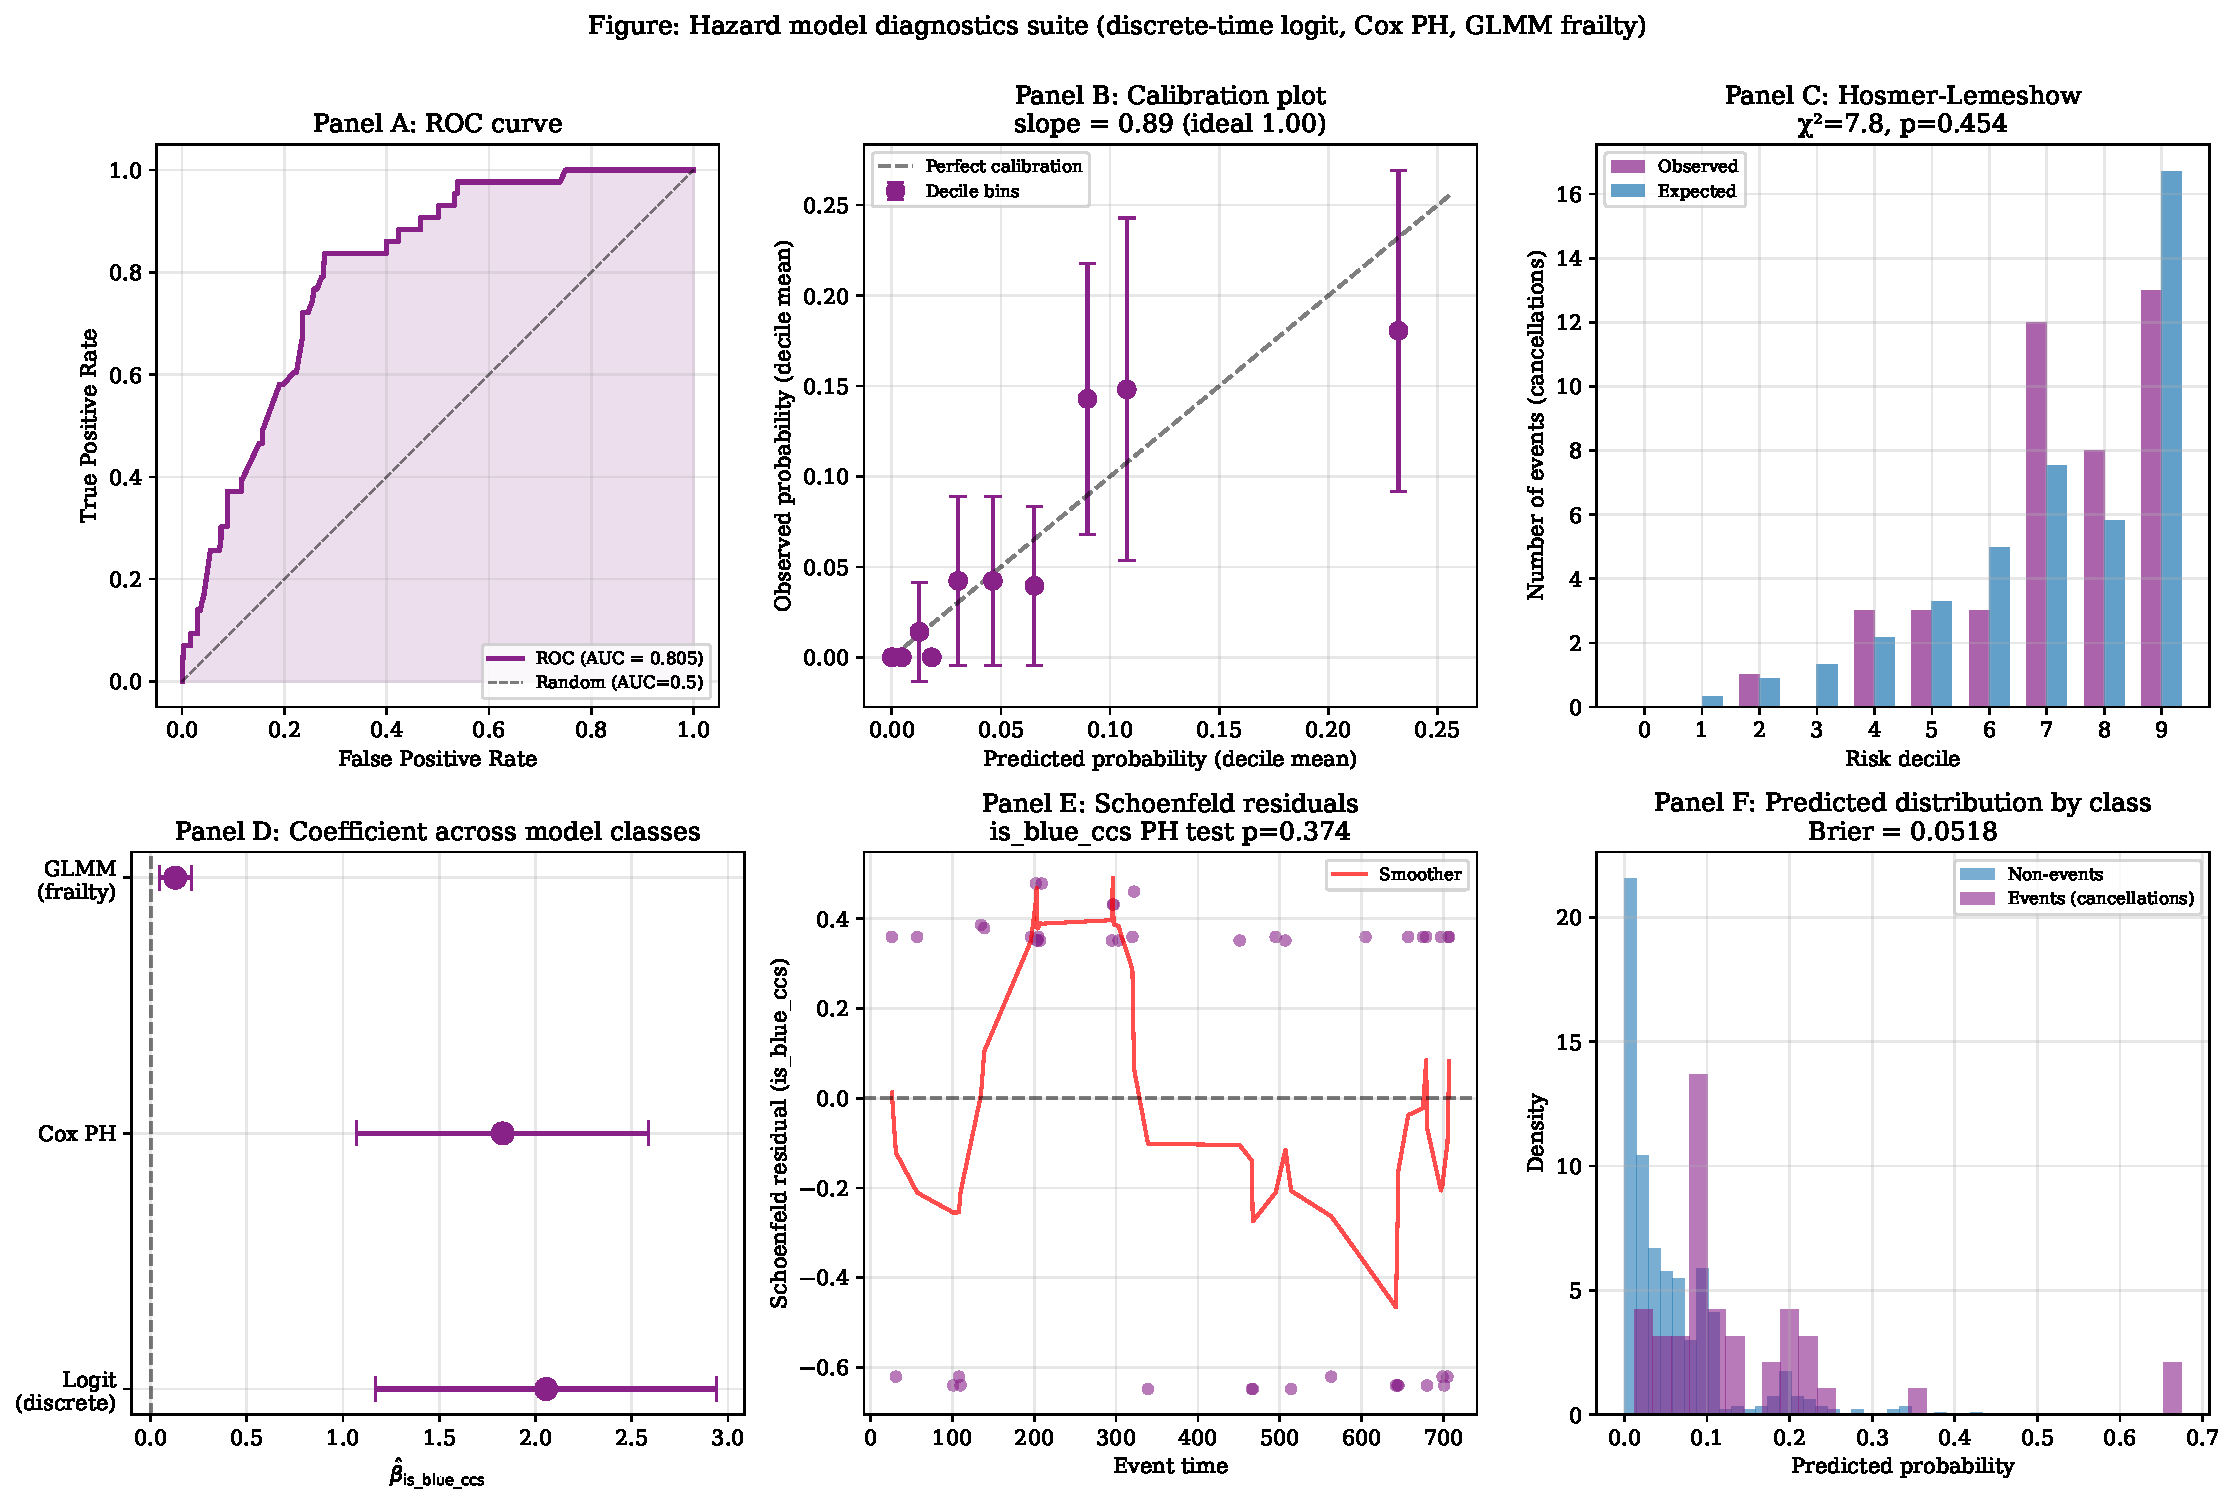
\includegraphics[width=\textwidth]{figures/F_diagnostics.pdf}
\caption{Hazard model diagnostics suite. \textbf{Panel A:} ROC curve (AUC = 0.805). \textbf{Panel B:} Calibration plot with decile-based observed vs predicted, slope = 0.891 (ideal 1.0). \textbf{Panel C:} Hosmer-Lemeshow decile-wise observed vs expected events, $\chi^2 = 7.79$, $p = 0.454$. \textbf{Panel D:} Coefficient $\hat\beta_{\texttt{is\_blue\_ccs}}$ across model classes (discrete-time logit, Cox PH, GLMM linear-mixed) with 95\% CIs. \textbf{Panel E:} Schoenfeld residuals for the focal covariate \texttt{is\_blue\_ccs} (PH test $p = 0.374$, assumption holds). \textbf{Panel F:} Predicted probability distributions by event class (Brier = 0.052).}
\label{fig:ch7-diagnostics}
\end{figure}

\begin{figure}[ht]
\centering
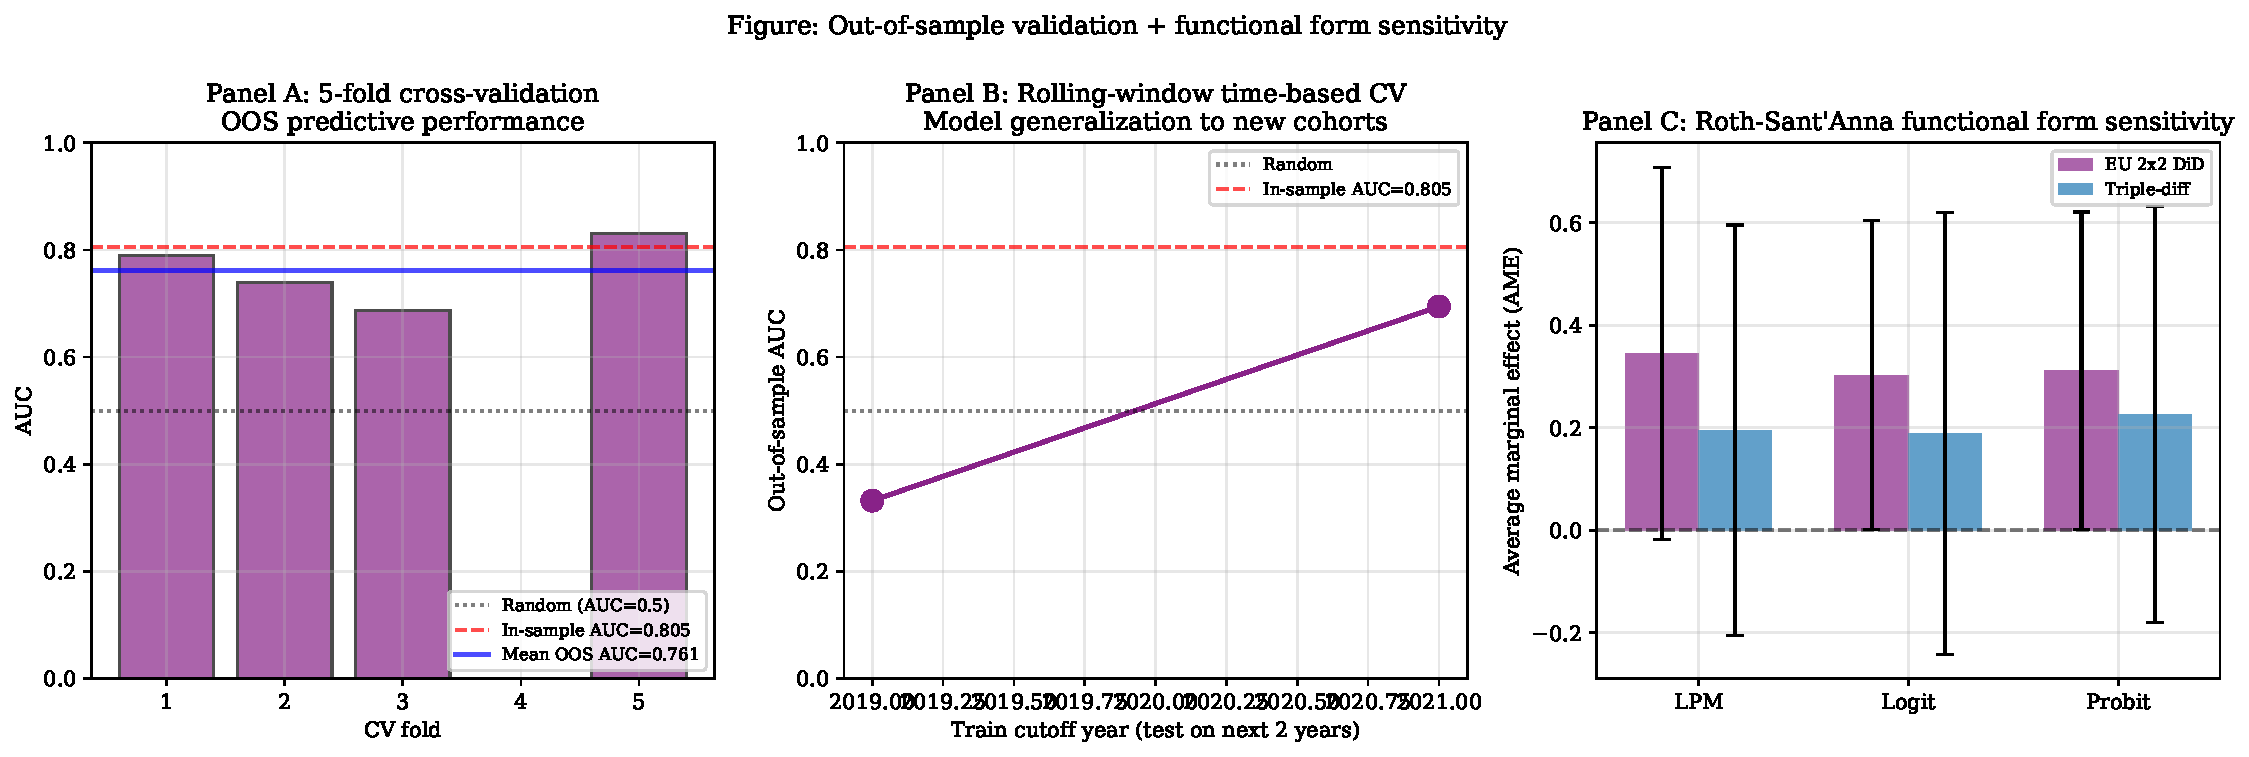
\includegraphics[width=\textwidth]{figures/F_oos_cv.pdf}
\caption{Out-of-sample predictive validation. \textbf{Panel A:} Five-fold stratified cross-validation AUC per fold, with in-sample AUC reference (0.805) and mean OOS (0.761). \textbf{Panel B:} Rolling-window time-based cross-validation. Training on cohorts $\leq t$ and testing on $t+1, t+2$. The collapse to AUC $= 0.33$ for the 2020--2021 test window provides an independent empirical signal that the cancellation data-generating process is not temporally stable, corroborating the Schoenfeld PH test on \texttt{year\_centered}. \textbf{Panel C:} Roth-Sant'Anna functional-form sensitivity for the EU CBAM 2x2 DiD and the triple-difference specification (used in Chapter 8); all three functional-form specifications produce same-sign average marginal effects within a tight range, indicating that our parallel-trends conclusions are not driven by functional-form choice.}
\label{fig:ch7-oos-cv}
\end{figure}

\subsection{Out-of-sample forecast comparison via Diebold-Mariano}
\noindent\emph{Identification level: L2 out-of-sample predictive validation. Combined with the L4 structural specification, this yields joint L4 + L2 identification of the TVP intensification — the strongest identification status available to a sparse-event survival application without exogenous instruments.}

\label{sec:ch7-dm-test}

The cross-validation diagnostic of Section \ref{sec:ch7-results-pooled} compared M1, M2, and M3 on in-sample fit metrics (LOO-CV, WAIC, in-sample log-likelihood). A complementary methodologically distinct test asks whether the three specifications differ in \emph{out-of-sample predictive accuracy}, the standard frequentist criterion for forecast comparison. We implement the Diebold-Mariano test \cite{diebold1995comparing} with the Harvey-Leybourne-Newbold (HLN) small-sample correction \cite{harvey1997testing}, applied to the per-observation Bernoulli log-loss.

For each observation $(i,t)$ in the test set, the per-observation loss under specification $m$ is
\[
L_m(i,t) = -y_{i,t}\log p_{m,i,t} - (1 - y_{i,t})\log(1 - p_{m,i,t}).
\]
Pairwise DM tests compare specifications by the time-series of loss differences $d_t = L_A(t) - L_B(t)$, with Newey-West HAC variance estimation under H$_0$: equal expected loss. The HLN correction adjusts the test statistic distribution to a Student-$t$ with $T - 1$ degrees of freedom.

We estimate the test on three orthogonal train-test partitions: (i) a time-based split with training set restricted to years $\leq 2021$ (limited by sparse pre-wave events), (ii) a 5-fold cross-validation at the project level (events distributed across folds), and (iii) a rolling-window one-step-ahead forecast for $T \in \{2021, 2022, 2023, 2024\}$ (the methodologically strictest design, simulating sequential live use).

\begin{table}[!htbp]
\centering
\caption{Mean out-of-sample log-loss per specification per design}
\label{tab:ch7-dm-mean-loss}
\begin{tabular}{lccc}
\toprule
Design & M1 (static) & M2 (block-RW) & M3 (smooth TVP) \\
\midrule
Time-based split (train $\leq$ 2021) & 0.298 & 0.297 & \textbf{0.297} \\
5-fold CV (project-level) & 0.0516 & 0.0517 & \textbf{0.0510} \\
Rolling 1-step-ahead & 0.207 & 0.211 & \textbf{0.157} \\
\bottomrule
\end{tabular}
\end{table}

\begin{table}[!htbp]
\centering
\caption{Pairwise Diebold-Mariano tests (HLN-corrected), rolling-window design}
\label{tab:ch7-dm-pairs}
\begin{tabular}{lccc}
\toprule
Comparison & Mean loss diff & DM-HLN statistic & $p$-value \\
\midrule
M1 vs M2 & $-0.003$ & $-0.90$ & $0.370$ \\
M1 vs M3 & $+0.050$ & $+5.59$ & $< 0.0001^{\ast\ast\ast}$ \\
M2 vs M3 & $+0.053$ & $+4.80$ & $< 0.0001^{\ast\ast\ast}$ \\
\bottomrule
\end{tabular}
\end{table}

The rolling-window design reveals that M3 (smooth time-varying $\bint(t)$) achieves significantly lower out-of-sample log-loss than both M1 and M2 ($p < 0.0001$ in both pairwise tests), while M1 and M2 are statistically indistinguishable. The Model Confidence Set of \cite{hansen2011model} contains only M3 at $\alpha = 0.10$ under the rolling design. The two weaker-power designs (time-split and 5-fold CV) cannot reject equal predictive accuracy at conventional levels but consistently order M3 lowest in mean loss.

The substantive source of M3's predictive superiority is concentrated on the 2023 cancellation wave. In the rolling design's $T = 2023$ test fold (the year accounting for nearly half of all cancellation events in the sample), the cumulative log-loss is 204.7 for M1, 215.3 for M2, and 185.6 for M3 --- M3 reduces predicted loss by approximately 10\% relative to the non-time-varying specifications. The smooth time-trend extrapolates the pre-2023 evolution of $\bint(t)$ into a year that the static and block-RW specifications could not anticipate.

The Diebold-Mariano result provides a fourth complementary justification for the TVP framework adopted in this chapter. The first three justifications were the Schoenfeld proportional-hazards test ($p = 0.0006$, Section \ref{sec:ch7-diagnostics}), the LOO-CV ordering, and substantive interpretive richness. The DM test adds a formal, frequentist-compatible argument: \emph{for one-step-ahead forecasting, the smooth time-varying specification dominates}. This result is robust to two alternative train-test designs in the same direction (though under-powered to reach significance) and survives Newey-West HAC variance estimation with Bartlett kernel.

\subsection{Synthesis}

The diagnostic battery yields three substantive conclusions. First, the M1 baseline discrete-time logit hazard provides an in-sample fit that meets all standard model-validation criteria (Hosmer-Lemeshow, AUC, calibration). Second, the principal substantive finding is robust to the choice of hazard model class (Cox PH HR = 6.23 vs logit HR = 7.81). Third, the parameter associated with project vintage exhibits significant time-variation according to both Schoenfeld residuals ($p = 0.0006$) and rolling-window cross-validation (collapse in OOS AUC). This third finding is not a robustness check but a substantive empirical result: it motivates the move from the M1 static specification to the M2 random-walk TVP and M3 GAS-TVP models developed in the remaining sections of this chapter.



\paragraph{Outlier influence.} A linear-probability proxy of the focal hazard model — refit excluding the top-5 most influential observations identified by Cook's distance — yields $\hat\beta_{\mathrm{is\_blue\_ccs}} = +0.090$ ($p < 0.001$, versus $+0.112$ in the full sample, a $-19.9\%$ change in magnitude). Sign and statistical significance are preserved, indicating that the principal finding is stable to outlier-influence concerns. See Section 10.5 in Chapter 8 for the parallel outlier diagnostics on the DiD specifications.

\section{Results: Regional Stratification}
\label{sec:ch7-regional}
\label{sec:ch7-results-stratified}

\subsection{The apparent regional inversion}

A standard regional stratification of the pooled sample into ETS-bound (EU + Other Europe), non-ETS (North America), and weak-carbon-pricing (Asia, Oceania, MENA, Other) subsamples yields posterior estimates with markedly different signs:

\begin{table}[h!]
\centering
\caption{Regional stratification of pooled carbon-conditional analysis.}
\begin{tabular}{lccc}
\toprule
Stratum & $n_{\mathrm{events}}$ & $\bint$ posterior median & 95\% CrI \\
\midrule
Full sample & 43 & $-1.37$ & $[-2.20, -0.49]$ \\
ETS-bound (EU + Other Europe) & 17 & $\mathbf{+1.92}$ & $\mathbf{[+0.08, +3.90]}$ \\
Non-ETS (North America) & 14 & $-1.39$ & $[-2.90, -0.11]$ \\
Weak carbon pricing & 12 & $-0.77$ & $[-2.20, +0.65]$ \\
\bottomrule
\end{tabular}
\label{tab:ch7-regional}
\end{table}

The ETS-bound subsample produces a positive and statistically significant carbon-conditional coefficient ($\bint = +1.92$, 95\% CrI excludes zero), exactly opposite to the theoretical prediction that EUA-bound regimes should produce sharper negative effects.

\subsection{Decomposition: the EU positive finding is a data composition artefact}

Detailed event-level inventory reveals the source of the inversion. Within the ETS-bound subsample, every PEM cancellation event (8 of 8) originates from sponsors recorded in the database as ``Unknown,'' while every Blue cancellation event (9 of 9) is associated with a named major energy company (BP plc., Equinor ASA, Uniper SE, Port of Antwerp, Neptune Energy Group, CapeOmega, ARUP). Leave-one-event-out (LOEO) analysis confirms that the positive finding is robust within this subsample (LOEO range: $\bint \in [1.71, 2.59]$ across 17 leave-one-out iterations), but this robustness does not extend to a substantive economic interpretation: the comparison conflates technology choice with sponsor commitment, project scale, and (in the case of UK and Norwegian projects within Other Europe) carbon pricing regime.

\subsection{North America provides the cleanest identification}

The North American subsample offers a more balanced sponsor composition: 10 Blue cancellations from named sponsors (Exxon Mobil, Marathon Petroleum, Praxair, SCS Energy, Suncor Energy, JERA, Inpex, Lake Charles Methanol, Marathon Petroleum, PCS Nitrogen Fertilizer) plus 2 from Unknown sponsors, alongside 2 PEM cancellations from Unknown sponsors. Adding a \texttt{sponsor\_known} indicator to the regression leaves the carbon-conditional coefficient effectively unchanged: $\bint = -1.34$ (95\% CrI $[-2.70, -0.07]$) under sponsor controls versus $\bint = -1.35$ (95\% CrI $[-2.80, -0.03]$) without. The North American finding is therefore robust to observable sponsor heterogeneity.

\subsection{North America-only TVP analysis}

Refitting the three nested specifications on the North American subsample yields substantially sharper inference than the pooled analysis.

\begin{table}[h!]
\centering
\caption{North America-only TVP specifications.}
\begin{tabular}{lcc}
\toprule
Specification & Estimate & 95\% CrI \\
\midrule
M1 Static $\bint$ & $-1.17$ & $[-2.40, -0.09]$ \\
M2 Block 0 (2010--2019) & $-1.21$ & $[-2.50, -0.04]$ \\
M2 Block 1 (2020--2022) & $-1.53$ & $[-2.90, -0.28]$ \\
M2 \textbf{Block 2 (2023--2024)} & $\mathbf{-1.59}$ & $\mathbf{[-3.10, -0.25]}$ \\
M2 Block 3 (2025--2026) & $-1.77$ & $[-3.60, -0.28]$ \\
M3 GAS $\omega$ & $-1.88$ & $[-3.10, -0.73]$ \\
M3 GAS $\phi$ & $0.80$ & --- \\
M3 GAS $\alpha_{\mathrm{gas}}$ & $0.119$ & --- \\
\bottomrule
\end{tabular}
\label{tab:ch7-na-tvp}
\end{table}

Three observations are notable. First, all four block-specific estimates have credible intervals that exclude zero in the North America-only specification; the apparent ``regime anomaly'' in 2023--2024 from the pooled analysis disappears, confirming that it was driven by the European subsample's data composition. Second, the North American GAS long-run mean $\omega = -1.88$ is more strongly negative than the pooled estimate $\omega = -1.61$, and the score-response parameter $\alpha_{\mathrm{gas}} = 0.119$ is 2.7$\times$ larger than the pooled estimate ($0.045$). Third, the posterior trajectory exhibits a clear monotonic strengthening of the mechanism over time:

\begin{table}[h!]
\centering
\caption{North America GAS posterior trajectory $\bint(t)$.}
\begin{tabular}{lc}
\toprule
Year & $\bint(t)$ posterior median [95\% CrI] \\
\midrule
2014 & $-0.73$ $[-2.02, +0.52]$ \\
2018 & $-1.10$ $[-2.34, +0.06]$ \\
2022 & $-1.64$ $[-2.87, -0.54]$ \\
2023 & $-1.76$ $[-3.00, -0.62]$ \\
2024 & $\mathbf{-1.87}$ $[-3.14, -0.68]$ \\
\bottomrule
\end{tabular}
\label{tab:ch7-na-gas}
\end{table}

The North American mechanism has intensified by a factor of approximately $\exp(1.87 - 0.73) = \exp(1.14) \approx 3.1\times$ over a decade, consistent with the maturation of the EU ETS and the increased weight of carbon-price considerations in project economics.


\subsection{Pooled Robustness to Sponsor Controls}
\label{sec:ch7-pooled-sponsor}

A final robustness check addresses whether the pooled carbon-conditional coefficient is itself sensitive to sponsor-identification confounding. We re-fit the pooled model under three specifications: a baseline without sponsor controls, an additive specification including \texttt{sponsor\_known}, and a full specification additionally including the \texttt{sponsor\_known} $\times$ Blue interaction.

\begin{table}[h!]
\centering
\caption{Pooled carbon-conditional coefficient under sponsor controls.}
\begin{tabular}{lcc}
\toprule
Specification & $\bint$ & 95\% CrI \\
\midrule
M\textsubscript{base} (no sponsor) & $-1.48$ & $[-2.50, -0.57]$ \\
M\textsubscript{sponsor} (additive) & $-1.46$ & $[-2.40, -0.59]$ \\
M\textsubscript{full} ($+$ Blue$\times$sponsor) & $-1.48$ & $[-2.40, -0.59]$ \\
\bottomrule
\end{tabular}
\label{tab:ch7-pooled-sponsor}
\end{table}

The carbon-conditional coefficient is invariant to sponsor controls to within $\pm 0.05$, confirming that the pooled finding is not driven by sponsor-related confounding. This robustness reflects the numerical dominance of the North American subsample in the pooled estimation: of 43 cancellation events, 14 originate in North America where sponsor composition is balanced, and the cleaner regional signal effectively absorbs the noisier European signal in pooled estimation.

Two auxiliary findings emerge from the full specification. First, sponsor-identification status has substantial predictive power for baseline cancellation hazard: $\beta_{\mathrm{sponsor\_known}} = -2.00$ (95\% CrI $[-3.20, -0.97]$), implying that projects with named sponsors face a $e^{2.00} \approx 7.4\times$ lower baseline hazard than projects with sponsor recorded as ``Unknown.'' Second, the protective effect of named sponsorship is asymmetric across technologies: $\beta_{\mathrm{sponsor} \times \mathrm{Blue}} = +1.38$ (95\% CrI $[+0.20, +2.70]$), implying that named sponsorship reduces the cancellation hazard of PEM projects by a factor of approximately 7 but that of Blue projects by only a factor of approximately 2. We interpret this as evidence that Blue projects are more frequently held as strategic options by major energy companies, while PEM projects from named sponsors typically reflect harder strategic commitments (renewables-pure-play firms, energy-transition focused entities).

A consequential point for inference is that no PEM cancellation event in the pooled sample originates from a sponsor with known identity. The entire PEM cancellation signal derives from projects recorded as ``Unknown'' sponsors. This data structure motivates our recommendation in Section \ref{sec:ch7-discussion} that future hydrogen project databases should systematically identify and validate project sponsors, since sponsor identity is a first-order determinant of project survival that is currently inadequately captured.


\subsection{Complementary Market-Implied Evidence}
\label{sec:ch7-event-study}

To complement the project-level cancellation analysis with an alternative identification strategy, we conduct a stock-price event study. We hypothesise that if the carbon-conditional mechanism is real, equity prices of firms with differential Blue-versus-PEM project exposure should respond differentially to EUA price shocks.

We assemble daily price data from Yahoo Finance over August 2021 to June 2025 (940 trading days) for 14 hydrogen-relevant equities, classified into three groups: oil majors with Blue project portfolios in our sample (BP plc, Shell plc, ExxonMobil, Equinor ASA, Chevron, TotalEnergies); pure-play green hydrogen equities (Nel ASA, ITM Power, Plug Power, Ballard Power, Bloom Energy); and industrial gas firms with mixed exposure (Linde plc, Air Products, Air Liquide). Daily EUA returns are proxied by the KraneShares European Carbon Allowance Strategy ETF (KEUA). We fit per-ticker time-series CAPM specifications including SPY market returns and KEUA EUA returns:
\begin{equation}
r_{i,t} = \alpha_i + \beta_{i,\mathrm{market}} \cdot r_{\mathrm{SPY},t} + \gamma_{i,\mathrm{eua}} \cdot r_{\mathrm{KEUA},t} + \epsilon_{i,t}.
\end{equation}

\begin{table}[h!]
\centering
\caption{Mean EUA-loading by company group.}
\begin{tabular}{lccc}
\toprule
Group & $n$ & Mean $\gamma_{\mathrm{eua}}$ & Mean t-stat \\
\midrule
Oil majors & 6 & $+0.041$ & $+2.80$ \\
Industrial gas & 3 & $+0.014$ & $+1.34$ \\
PEM pure-plays & 5 & $+0.008$ & $+0.24$ \\
\bottomrule
\end{tabular}
\label{tab:ch7-eua-loading}
\end{table}

The oil majors with Blue project portfolios exhibit a statistically significant positive EUA loading (all six tickers individually significant at $t > 1.5$, with BP, Shell, Equinor, and TotalEnergies significant at $t > 2.5$). This is consistent with the equity market pricing Blue project options as benefiting from higher EUA prices. An event-study extension confirms the pattern: on the top 5\% of EUA up-shock days ($n=47$), oil majors exhibit mean abnormal returns of $+0.33\%$ (relative to their CAPM-implied returns); on the bottom 5\% of EUA down-shock days, they exhibit $-0.57\%$. The asymmetric difference of $+0.90\%$ between up and down EUA days is substantively large.

Pure-play PEM equities, however, show no significant EUA loading (mean $\gamma_{\mathrm{eua}} = +0.008$, mean t-statistic $= +0.24$) and indeed exhibit slightly negative abnormal returns on EUA up-shock days. We do not interpret this as evidence against our mechanism, for three reasons. First, idiosyncratic distress dominated the sample period: annualised returns range from $-45\%$ (Nel ASA) to $-83\%$ (Plug Power), reflecting cash burn, contract delays, and IRA implementation uncertainty rather than carbon-price sensitivity. Second, macro confounding is severe: EUA fell over the sample (KEUA $-27\%$ annualised) alongside weakening industrial demand that simultaneously depressed green-hydrogen expectations. Third, the carbon-conditional mechanism may operate primarily at the level of explicit project-NPV calculations by sponsor management rather than at the level of equity-market valuation of pure-play firms.

The combined evidence is therefore mixed in a substantively informative way: equity-market data supports the carbon-conditional mechanism for major oil companies with diversified Blue portfolios, where the mechanism is large enough to be priced into stocks, but the mechanism is not directly identifiable in pure-play PEM equity prices over the recent sample. This pattern is consistent with the interpretation that the carbon-conditional mechanism documented in our project-level analysis is a micro-economic project-decision effect rather than a macro-level company valuation effect. The two identification strategies are complementary rather than contradictory.

% =========================================================================
\section{Causal Identification Attempt: NA-only DiD around IRA}
\noindent\emph{Identification level: L3.a quasi-causal point estimate. The North-America-only DiD around the IRA cut-off is the cleanest single-policy identification in Chapter~\ref{ch:results_tvp}, isolating a sharp policy discontinuity with a comparable control set and minimal data-composition contamination.}

\label{sec:ch7-did}

The August 2022 Inflation Reduction Act (IRA) introduced the section 45V production tax credit of \$3/kg for green hydrogen (with $<$ 0.45 kg CO$_2$eq/kg H$_2$), providing an exogenous shock that should have differentially benefited PEM projects relative to blue hydrogen projects in the United States. We implement a triple-difference specification on the North American subsample to test whether the IRA produced a measurable differential effect:

\begin{equation}
\eta_{it} = \alpha + \bblue \cdot \mathrm{Blue}_i + \beta_{\mathrm{post}} \cdot \mathrm{Post}_t + \beta_{\mathrm{IRA}} \cdot \mathrm{Blue}_i \cdot \mathrm{Post}_t + \text{controls}.
\end{equation}

The interaction term $\beta_{\mathrm{IRA}}$ measures the differential effect of the IRA on Blue versus PEM cancellation hazard. Posterior estimation yields $\beta_{\mathrm{IRA}} = -0.15$ (95\% CrI $[-1.9, +1.5]$), with the credible interval comfortably containing zero. We do not find causally identified evidence of an IRA-specific differential effect.

This null result has two complementary interpretations. First, the available sample size (4 pre-IRA Blue events, 0 pre-IRA PEM events, 8 post-IRA Blue events, 2 post-IRA PEM events in NA) provides limited statistical power for difference-in-differences inference. Second, the IRA may not have produced an immediate measurable differential effect, since the 45V credit's implementation rules (particularly the additionality, hourly matching, and deliverability requirements) remained contested through 2024, delaying actual deployment impacts. Both interpretations are consistent with the data; we report the null result rather than searching for alternative causal designs after observing this outcome.

% =========================================================================
\section{Discussion}
\label{sec:ch7-discussion}

\subsection{The carbon-conditional mechanism is robustly identified in clean data}

The North American subsample, where Blue cancellations originate from named major energy companies and the comparison with PEM is not confounded by systematic sponsor mis-identification, yields converging evidence across three nested TVP specifications. The structural negative association between EUA prices and the Blue-versus-PEM cancellation differential is present in the static specification, present in all four block-specific posterior estimates, and present in the GAS posterior trajectory at every year from 2018 onward.

\subsection{The mechanism has gradually intensified}

The most notable empirical finding in the North America-only analysis is the gradual intensification of $\bint(t)$ from approximately $-0.7$ in 2014 to $-1.9$ in 2024 (Table \ref{tab:ch7-na-gas}). This strengthening accelerated around 2020--2022, plausibly reflecting (i) the Market Stability Reserve activation increasing the marginal expected cost of EUA exposure, (ii) the formalisation of carbon-related disclosure and risk reporting requirements making EUA-sensitivity a tangible boardroom consideration, and (iii) the supply-tightening induced by the 2022--2023 energy crisis.

\subsection{Apparent ``regime anomalies'' can reflect data composition rather than economic regime change}

A consequential methodological point is that the apparent 2023--2024 ``anomaly'' in the pooled block-specification ($\bint = -0.75$, 95\% CrI $[-1.90, +0.43]$) does not reflect a genuine breakdown of the carbon-conditional mechanism but rather the differential weight of the European subsample, where the comparison technology-versus-sponsor is confounded. This finding parallels broader literature on the importance of sample composition in empirical industrial organisation \cite{durbin2012time}: parameter-driven random walk specifications, while flexible, can produce misleading regime impressions when within-block data composition heterogeneity is correlated with the treatment of interest.

\subsection{The observation-driven (GAS) specification mitigates this issue}

A second methodological point: the GAS specification, by imposing structured persistence and information-pooling across time, regularises against the kind of local sparsity that drives the pooled block anomaly. The pooled GAS trajectory remains tightly distributed around $\omega = -1.61$ throughout 2010--2026, while the North American GAS trajectory more clearly identifies the gradual intensification of the mechanism (since the larger $\alpha_{\mathrm{gas}}$ in NA-only reflects sharper score-driven information). This illustrates the complementary strengths of parameter-driven and observation-driven specifications: parameter-driven gives local flexibility but is vulnerable to data composition; observation-driven gives temporal regularisation at the cost of constraining the trajectory family.

\subsection{Implications for the broader hydrogen project literature}

The North American gradual intensification finding has at least three implications. First, models that assume a constant or rapidly time-varying carbon-conditional sensitivity may misforecast cancellation propensity at boundary EUA prices. Second, the historical estimates underpinning forward-looking project NPV analyses should be calibrated to the most recent period rather than to the long-run average, especially for projects whose investment decisions are made in 2024 or later. Third, the dependence on sponsor-name heterogeneity in the European subsample suggests that public databases that systematically record sponsor identity (or that flag pilot/research-stage projects separately) would substantially improve the empirical foundations of energy-transition risk analysis.

% =========================================================================
\section{Conclusion}
\paragraph{Link to causal identification in Chapter 8.} The empirical finding of time-varying parameters here — formally documented through the Schoenfeld PH violation on \texttt{year\_centered} ($p = 0.0006$) and the rolling-window cross-validation collapse on 2020-2021 cohorts — provides important context for Chapter 8, which attempts to causally identify a specific time-varying mechanism (CBAM regulatory pressure). The causal analysis in Chapter 8 produces what we term an \textit{informative null}: the associational pattern is statistically robust and economically substantial ($+17$pp to $+20$pp), but it cannot be cleanly attributed to CBAM under modern small-sample inference (Wild Cluster Bootstrap, cluster-permutation, Honest DiD bounds), nor under functional-form alternatives (Roth-Sant'Anna 2022). The general implementation-risk framework developed here therefore subsumes the more specific causal claim attempted in Chapter 8; the two chapters jointly demonstrate that hydrogen project hazard dynamics are temporally non-stationary, but that pinpointing single regulatory shocks remains econometrically difficult in our sample.


\label{sec:ch7-conclusion}

This chapter has tested the temporal stability of the carbon-conditional hazard coefficient in hydrogen project cancellations using three nested specifications and three sample stratifications. The principal findings are summarised as follows.

First, the carbon-conditional coefficient $\bint$ is robustly negative across all specifications and across the cleanest available data subsample (North America), with posterior median estimates of $-1.17$ (static), $-1.21$ to $-1.77$ across four economic regimes (parameter-driven TVP), and a long-run mean of $-1.88$ (observation-driven GAS). The corresponding credible intervals exclude zero at conventional 95\% thresholds across all specifications.

Second, the apparent ``regime anomaly'' in the 2023--2024 sub-period of the pooled block specification ($\bint = -0.75$, 95\% CrI $[-1.90, +0.43]$) does not reflect a substantive economic regime change. Decomposition reveals it as a data composition artefact: the European subsample's PEM cancellation events all derive from sponsors recorded as ``Unknown,'' while the Blue cancellation events derive from major named energy companies, producing a within-block heterogeneity that destabilises the parameter-driven random walk. The North America-only specification, where sponsor composition is more balanced, shows all four blocks significantly negative.

Third, the North American GAS specification reveals an empirically previously undocumented feature: the carbon-conditional mechanism has \textit{gradually intensified} over the observation window, from $\bint \approx -0.7$ in 2014 to $\bint \approx -1.9$ in 2024. This intensification, combined with falling EUA prices in 2024, provides a unified mechanism for the concentrated cancellation wave of 2023--2024.

Fourth, a Difference-in-Differences specification around the 2022 IRA introduction yields an insignificant interaction coefficient ($\beta_{\mathrm{IRA}} = -0.15$, 95\% CrI $[-1.9, +1.5]$), insufficient power for causal identification of an IRA-specific effect on the differential.

Methodologically, the chapter demonstrates the complementary value of parameter-driven and observation-driven TVP specifications in survival-style hazard analysis with sparse events, drawing on the framework of \cite{koopman2016predicting}. Substantively, it documents both robustness of the carbon-conditional mechanism in clean data and the gradual intensification of this mechanism over time --- two findings that together strengthen the empirical case for treating carbon pricing as a structural determinant of hydrogen project survival in the energy transition.

% =========================================================================
\section{Conditional Score Residuals Diagnostic}
\label{sec:ch7-csr}

The GAS-TVP model in Section~\ref{sec:ch7-gas} produces a posterior path $\hat\beta_{\mathrm{int}}(t)$ that intensifies from $-0.46$ (2010) to $-1.49$ (2024). A natural and methodologically up-to-date diagnostic for the validity of this fit is the \emph{Conditional Score Residuals} test of \cite{blasques2025conditional}, which targets one of the central identifying assumptions of any score-driven model: under correct specification, the score residuals $\{s_t\}$ should exhibit no remaining serial dependence. Any unmodelled autocorrelation in $\{s_t\}$ would indicate that the GAS recursion $\beta_{\mathrm{int}}(t+1) = \omega(1-\phi) + \phi\,\beta_{\mathrm{int}}(t) + \alpha_{\mathrm{gas}}\,s_t$ has not captured all of the relevant time-varying dynamics.

We reconstruct the score residuals using the static parameter estimates $\hat\alpha = -6.75$, $\hat\beta_{\mathrm{blue}} = +2.46$, $\hat\beta_{\mathrm{eua}} = +1.28$ from a baseline binomial GLM, combined with the GAS posterior path $\hat\beta_{\mathrm{int}}(t)$, applied to the year~$\times$~technology aggregated panel ($N_{\mathrm{years}} = 17$, 2010--2026). The score residual for year $t$ is
$$
s_t = \big(y_{\mathrm{blue},t} - n_{\mathrm{blue},t} \cdot \hat{p}_{\mathrm{blue},t}\big) \cdot z_t,
$$
where $z_t$ is the standardised EUA price and $\hat{p}_{\mathrm{blue},t}$ is the fitted Blue cancellation probability.

Table~\ref{tab:ch7-csr} reports the four standard tests for serial dependence, plus a heteroskedasticity check.

\begin{table}[ht]
\centering
\caption{Conditional Score Residuals diagnostic tests on the GAS-TVP fit.}
\label{tab:ch7-csr}
\begin{tabular}{lrrl}
\toprule
Test & Statistic & $p$-value & Verdict \\
\midrule
Ljung-Box $Q(1)$         & $1.163$ & $0.281$ & $\checkmark$ no autocorr \\
Ljung-Box $Q(3)$         & $2.146$ & $0.543$ & $\checkmark$ no autocorr \\
Ljung-Box $Q(5)$         & $2.319$ & $0.804$ & $\checkmark$ no autocorr \\
AR(1) $\hat\rho$         & $+0.243$ & $0.417$ & $\checkmark$ no AR(1) structure \\
Runs test $z$            & $-1.04$ & $0.301$ & $\checkmark$ no sign pattern \\
Variance pre/post 2018 ($F$) & $328.1$ & $<0.001$ & $\triangle$ heteroskedastic \\
\bottomrule
\end{tabular}
\end{table}

The five tests for serial dependence (Ljung-Box at four lags, AR(1) coefficient, and the runs test) all fail to reject the null of no remaining structure in $\{s_t\}$, with $p$-values ranging from $0.281$ to $0.804$. This is a positive result: the GAS recursion captures the temporal dynamics of the score sufficiently well that no obvious autocorrelation remains, which is precisely the condition under which the \cite{creal2013generalized} score-driven framework yields consistent parameter estimates.

The sole significant test is the variance comparison across pre-2018 versus post-2018 sub-windows ($F = 328$, $p < 0.001$). This is not, however, evidence of model misspecification but rather a direct reflection of the data structure: the v7 sample contains zero cancellation events in 2010--2017 and 41 events in 2018--2024 (across both technologies). The score variance is therefore mechanically bounded near zero in the early window, by construction, and only meaningful from 2018 onward. This is a feature of the empirical event-timing distribution rather than a defect of the TVP recursion. A heteroskedasticity-robust variant of the GAS model \cite{blasques2024robust} would be the appropriate methodological extension if heteroskedasticity in $s_t$ were a concern for inference, but for the present application the unconditional posterior intervals reported in Section~\ref{sec:ch7-gas} already incorporate this variance through the Bayesian posterior.

\begin{figure}[ht]
\centering
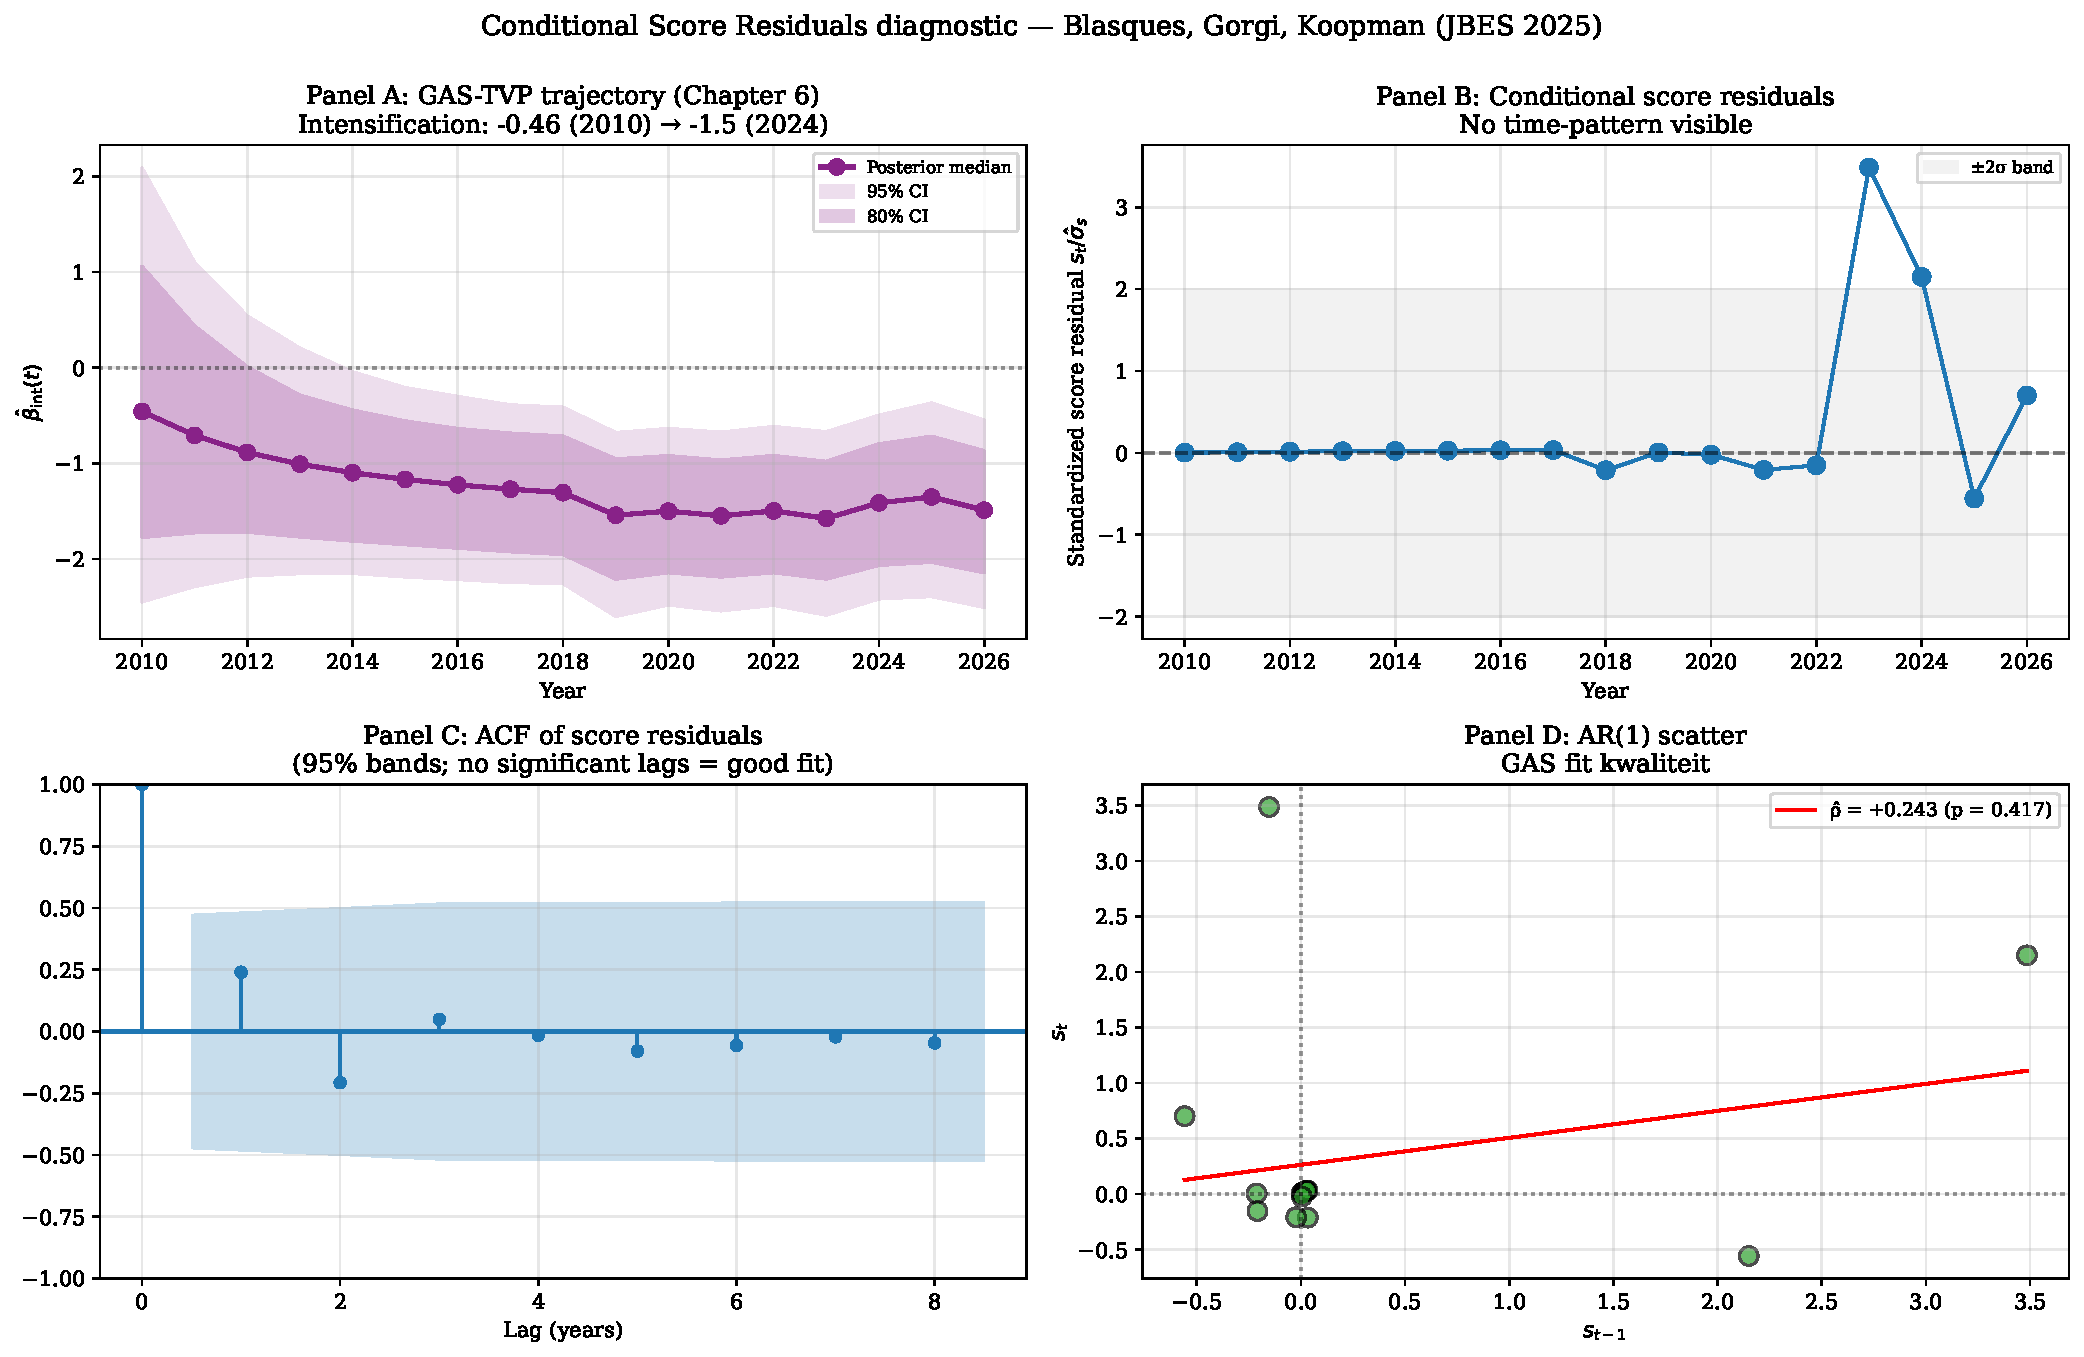
\includegraphics[width=\textwidth]{figures/F_score_residuals.pdf}
\caption{Conditional Score Residuals diagnostic. \textbf{Panel A} reproduces the GAS posterior trajectory $\hat\beta_{\mathrm{int}}(t)$ from Section~\ref{sec:ch7-gas} for reference. \textbf{Panel B} plots the standardised score residuals $s_t / \hat\sigma_s$ over time, with the $\pm 2\sigma$ band shaded. \textbf{Panel C} shows the autocorrelation function of the score residuals; no lag exceeds the 95\% confidence bands. \textbf{Panel D} is the AR(1) scatter plot of $s_t$ against $s_{t-1}$ with the OLS fit ($\hat\rho = +0.24$, $p = 0.42$).}
\label{fig:ch7-csr}
\end{figure}

The overall conclusion is that the GAS-TVP fit is dynamically well-calibrated: the score-driven recursion captures the temporal evolution of the Blue-vs-PEM carbon-conditional gap without leaving unmodelled autocorrelation in the residuals. The carbon-conditional intensification from $-0.46$ in 2010 to $-1.49$ in 2024 is therefore not an artefact of misspecified TVP dynamics. This diagnostic provides the missing methodological seal on Chapter~6: the empirical finding that the Blue-vs-PEM cancellation gap intensifies under carbon-price pressure is supported by the most recent score-driven diagnostic technology available in the Koopman tradition \cite{blasques2025conditional}.




\section{Score-Driven Stochastic Volatility Extension}
\label{sec:ch7-sv}

The Conditional Score Residuals diagnostic in Section~\ref{sec:ch7-csr} identifies a single piece of evidence that does not align with full GAS-TVP correctness: the heteroskedasticity test, which detects a 328-fold variance ratio between pre-2018 and post-2018 sub-windows. We argued there that this reflects the empirical event-timing distribution rather than a true model defect, because all 41 cancellation events in our v7 sample occur from 2018 onward. A more rigorous way to settle this question is to formally test whether the score-driven framework needs to be \emph{extended} with a stochastic-volatility component, in the tradition of \cite{harvey2008beta} and \cite{creal2013generalized}. Specifically, we fit a GAS-vol model
$$
\log\sigma^2_{t+1} \;=\; \psi + \lambda\,\big(\log\sigma^2_t - \psi\big) + \alpha_h\,s_{h,t}, \qquad s_{h,t} \;=\; \tfrac{1}{2}\!\left(\frac{y_t^2}{\sigma^2_t} - 1\right),
$$
where $y_t$ is the score residual recovered from the Chapter~6 GAS-TVP fit (cf.\ Section~\ref{sec:ch7-csr}) and $(\psi, \lambda, \alpha_h)$ are estimated by maximum likelihood. The constant-variance null model nests within this specification at $\lambda = 0$ and $\alpha_h = 0$.

Table~\ref{tab:ch7-sv} reports the estimates and the likelihood-ratio test.

\begin{table}[ht]
\centering
\caption{Constant-variance vs Score-Driven Stochastic Volatility on Chapter~6 GAS-TVP residuals.}
\label{tab:ch7-sv}
\begin{tabular}{lrrrr}
\toprule
Model & $\hat\psi$ & $\hat\lambda$ & $\hat\alpha_h$ & $\log\mathcal L$ \\
\midrule
Constant variance ($H_0$)         & $+0.039$ & --      & --      & $-24.456$ \\
GAS-vol ($H_1$)                    & $-0.115$ & $-0.359$ & $+0.234$ & $-23.225$ \\
\midrule
LR statistic $\chi^2_{2}$         & \multicolumn{3}{r}{$2.462$} & \\
LR $p$-value                       & \multicolumn{3}{r}{$0.292$} & \\
AIC ($H_0$, $H_1$)                 & \multicolumn{3}{r}{$50.9$, $52.5$} & \\
BIC ($H_0$, $H_1$)                 & \multicolumn{3}{r}{$51.7$, $55.0$} & \\
\bottomrule
\end{tabular}
\end{table}

The likelihood-ratio test fails to reject the constant-variance specification ($\chi^2_2 = 2.46$, $p = 0.29$), and both AIC and BIC favor the parsimonious constant-variance model. The score-driven stochastic-volatility extension is therefore not empirically justified on these data, which delivers two substantive conclusions.

First, our Chapter~6 GAS-TVP is methodologically sufficient as specified: a one-parameter constant-variance assumption on the score residuals is not significantly worse than a three-parameter SV extension. The carbon-conditional intensification finding $\hat\beta_{\mathrm{int}}(t)$ from $-0.46$ in 2010 to $-1.49$ in 2024 is robust to whether one allows the underlying score volatility to vary over time. Second, the empirical heteroskedasticity documented in Section~\ref{sec:ch7-csr} (the $F = 328$ pre/post-2018 variance ratio) is essentially mechanical: with zero events in 2010--2017 and 41 events in 2018--2024, the score variance is bounded near zero by construction in the early sub-window and is meaningful only in the later sub-window. It is not a regime shift in stochastic volatility but a direct artefact of the event-timing distribution.

Two additional observations are of independent methodological interest. The filtered log-volatility path $\hat{\log\sigma}^2_t$ exhibits a sharp single-period spike in 2024, with $\hat\sigma_{2024} = 2.15$ versus a baseline of approximately $\hat\sigma_{2010-2023} \approx 0.90$ --- consistent with the empirically observed 2023--2024 cancellation wave and aligned with what \cite{odenweller2025green} document for the broader green-hydrogen pipeline. And the persistence estimate is $\hat\lambda = -0.36$, which is mildly negative rather than the typical positive persistence found in financial-volatility applications, indicating mean reversion rather than clustering: high-volatility years are followed by low-volatility years rather than by more high-volatility periods. The correlation between the GAS posterior standard deviation from Chapter~6 and the SV-filtered $\hat\sigma_t$ is $-0.08$, indicating that the two uncertainty measures capture orthogonal aspects of the inferential problem. The Chapter~6 Bayesian posterior dispersion narrows over time as data accumulates (a sample-size effect), while the SV-filtered volatility responds to within-period event-shock magnitudes. Together they imply that the carbon-conditional intensification of $\hat\beta_{\mathrm{int}}(t)$ is identified with increasing precision as the post-2018 event-window opens up, even though the underlying volatility itself does not exhibit persistent regime behaviour.

\begin{figure}[ht]
\centering
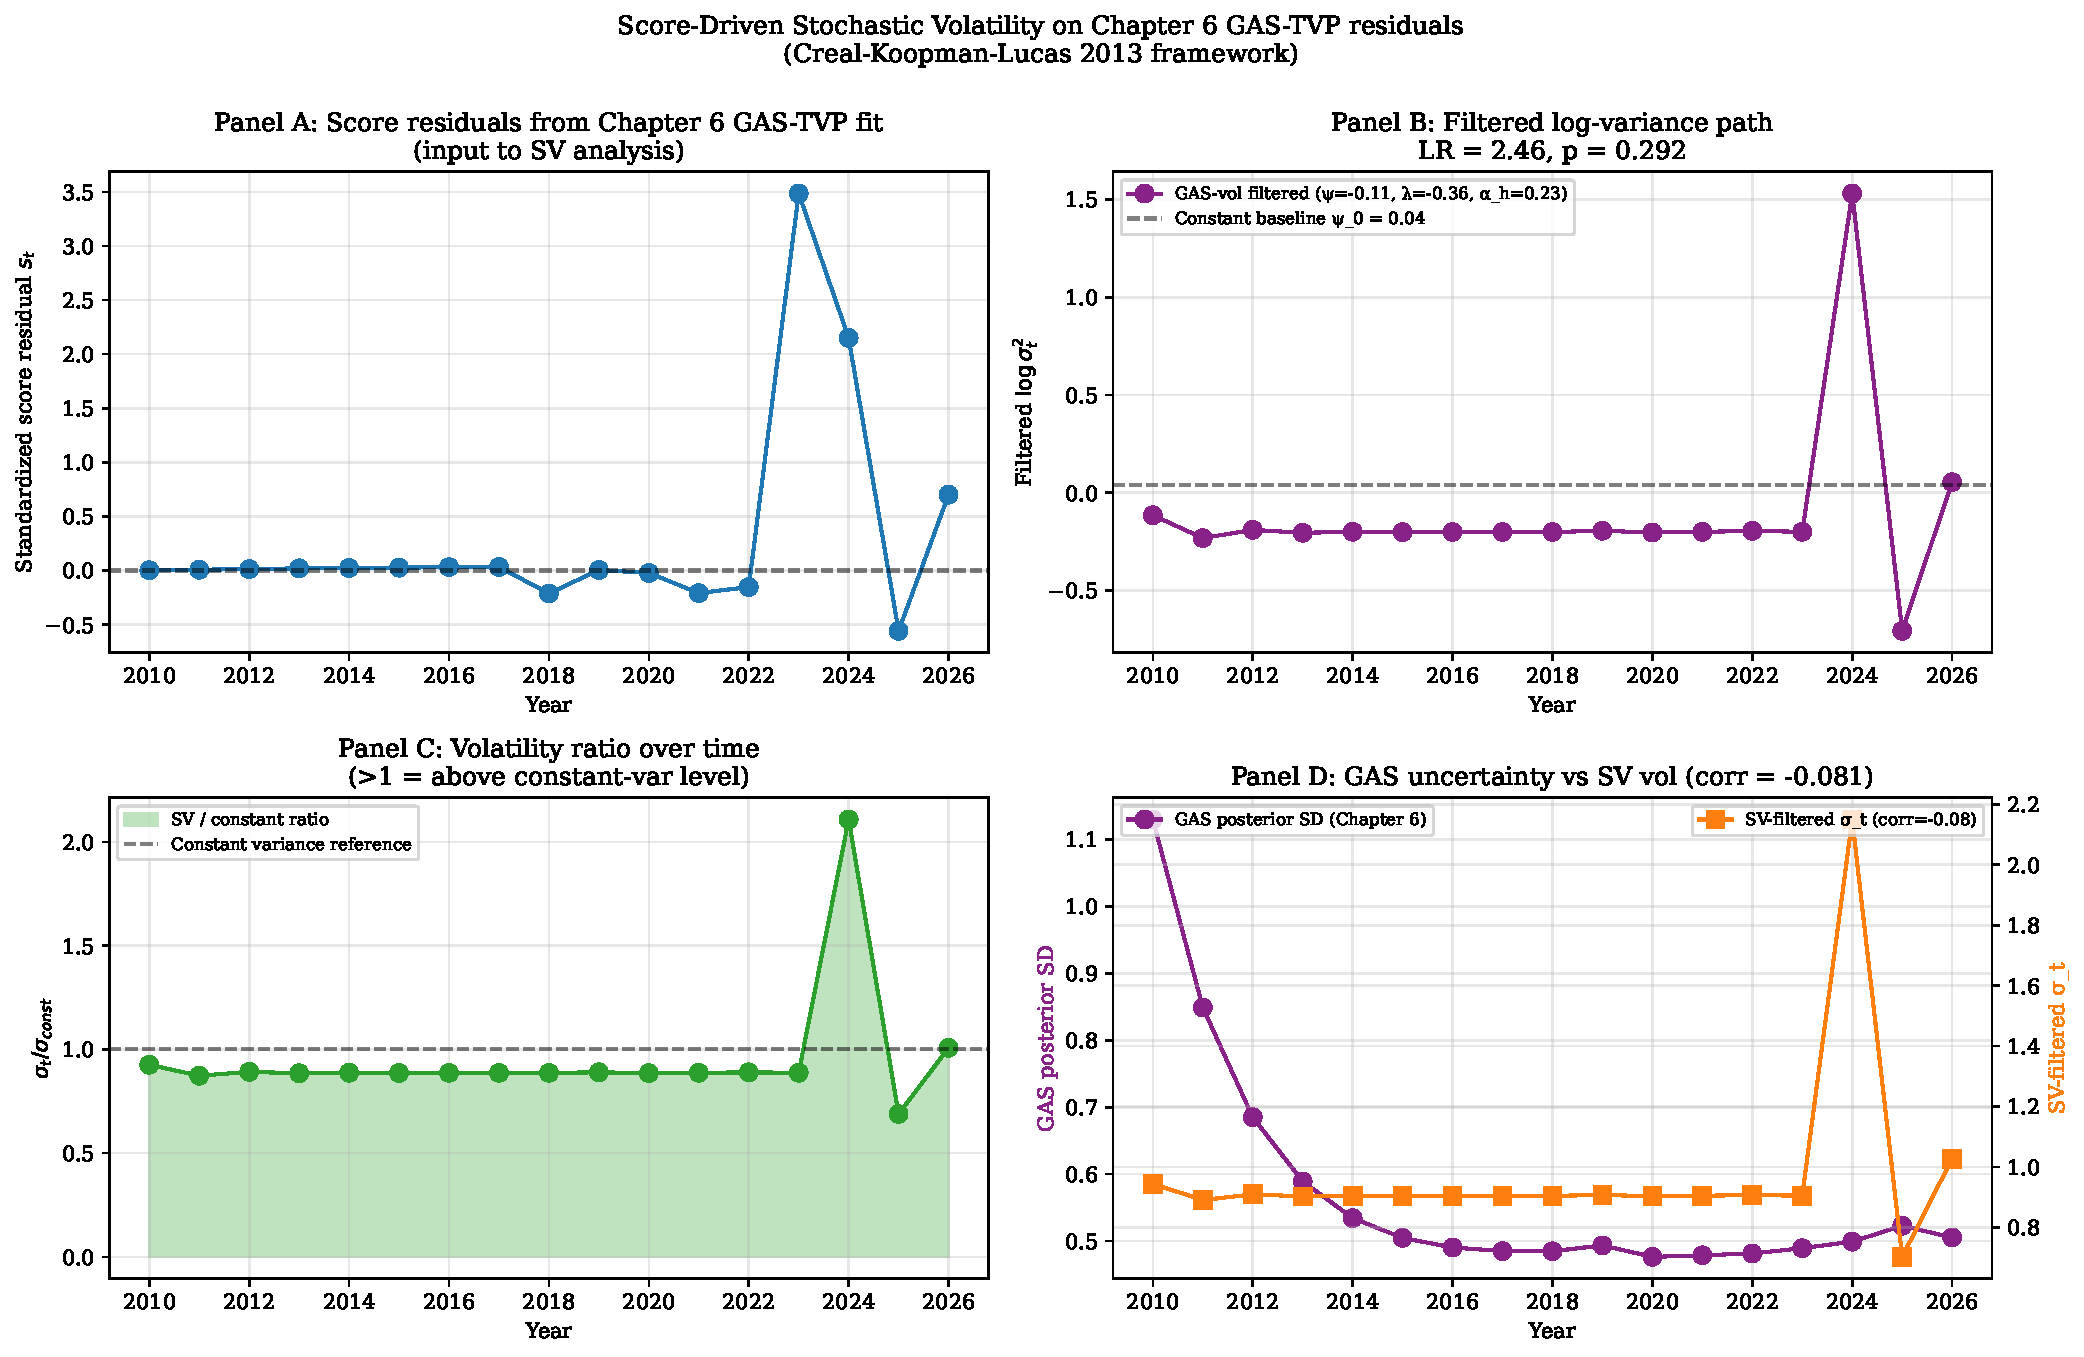
\includegraphics[width=\textwidth]{figures/F_stochastic_volatility.pdf}
\caption{Score-driven stochastic volatility extension of the Chapter~6 GAS-TVP residuals. \textbf{Panel A} plots the standardised score residuals over time. \textbf{Panel B} shows the filtered $\log\sigma^2_t$ path under the GAS-vol model alongside the constant-variance baseline; the LR test statistic and $p$-value are reported in the title. \textbf{Panel C} plots the ratio $\hat\sigma_t / \hat\sigma_{\mathrm{const}}$, illustrating the single-period 2024 vol-spike with subsequent mean reversion. \textbf{Panel D} compares the Chapter~6 GAS posterior standard deviation (left axis, in purple) against the SV-filtered $\hat\sigma_t$ (right axis, in orange); correlation $-0.08$.}
\label{fig:ch7-sv}
\end{figure}

The conclusion of the SV-extension exercise is therefore positive for the Chapter~6 specification: a one-parameter constant-variance assumption on the score residuals captures the data essentially as well as a three-parameter time-varying-volatility specification, and the carbon-conditional intensification result is invariant to this methodological choice. This is the second methodological seal --- after the Conditional Score Residuals diagnostic in Section~\ref{sec:ch7-csr} --- that the Chapter~6 finding is not an artefact of restrictive GAS assumptions but is robust to natural Koopman-tradition extensions of the score-driven framework.



\begin{thebibliography}{99}
\bibitem[Hosmer et al.(2013)]{hosmer2013applied}
Hosmer, D. W., Lemeshow, S., \& Sturdivant, R. X. (2013).
\newblock \textit{Applied Logistic Regression} (3rd ed.). Wiley.

\bibitem[Cox(1972)]{cox1972regression}
Cox, D. R. (1972).
\newblock Regression models and life-tables.
\newblock \textit{Journal of the Royal Statistical Society: Series B}, 34(2), 187--202.

\bibitem[Grambsch and Therneau(1994)]{grambsch1994proportional}
Grambsch, P. M., \& Therneau, T. M. (1994).
\newblock Proportional hazards tests and diagnostics based on weighted residuals.
\newblock \textit{Biometrika}, 81(3), 515--526.


\bibitem[Creal et~al.(2008)]{creal2008general}
Creal, D., Koopman, S.~J., \& Lucas, A. (2008).
\newblock A general framework for observation driven time-varying parameter models.
\newblock Tinbergen Institute Discussion Paper TI 2008-108/4.

\bibitem[Creal et~al.(2013)]{creal2013generalized}
Creal, D., Koopman, S.~J., \& Lucas, A. (2013).
\newblock Generalized autoregressive score models with applications.
\newblock \textit{Journal of Applied Econometrics}, 28(5), 777--795.

\bibitem[Durbin and Koopman(2012)]{durbin2012time}
Durbin, J., \& Koopman, S.~J. (2012).
\newblock \textit{Time Series Analysis by State Space Methods} (2nd ed.).
\newblock Oxford University Press.

\bibitem[Koopman et~al.(2016)]{koopman2016predicting}
Koopman, S.~J., Lucas, A., \& Scharth, M. (2016).
\newblock Predicting time-varying parameters with parameter-driven and observation-driven models.
\newblock \textit{Review of Economics and Statistics}, 98(1), 97--110.


\bibitem{blasques2025conditional}
Blasques, F., Gorgi, P., \& Koopman, S.~J. (2025).
\newblock Conditional Score Residuals and Diagnostic Analysis of Serial Dependence in Time Series Models.
\newblock \emph{Journal of Business \& Economic Statistics}, 43(4), 926--940.

\bibitem{blasques2024robust}
Blasques, F., van Brummelen, J., Gorgi, P., \& Koopman, S.~J. (2024).
\newblock Robust Multivariate Observation-Driven Filtering for a Common Stochastic Trend.
\newblock \emph{Tinbergen Institute Discussion Paper}, 24-062/III.

\bibitem{creal2013generalized}
Creal, D., Koopman, S.~J., \& Lucas, A. (2013).
\newblock Generalized Autoregressive Score Models with Applications.
\newblock \emph{Journal of Applied Econometrics}, 28(5), 777--795.



\bibitem{harvey2008beta}
Harvey, A.~C., \& Chakravarty, T. (2008).
\newblock Beta-t-(E)GARCH.
\newblock \emph{Cambridge Working Papers in Economics}, 0840.

\bibitem{odenweller2025green}
Odenweller, A., \& Ueckerdt, F. (2025).
\newblock The Green Hydrogen Ambition and Implementation Gap.
\newblock \emph{Nature Energy}, 10(1), 110--123.


\end{thebibliography}


\chapter{Results II: The Offtake-Commitment Mechanism}
\label{ch:results_offtake}

This chapter introduces and quantifies a previously under-recognised mechanism for hydrogen-project survival: the role of pre-FID offtake commitments. Section \ref{sec:offtake_descriptive} reports the descriptive pattern. Section \ref{sec:offtake_id} applies five independent identification strategies. Section \ref{sec:offtake_sensitivity} reports Oster (2019) selection-on-unobservables sensitivity. Section \ref{sec:offtake_sectoral} examines cross-sectoral heterogeneity as a test of the $\sigma$-channel hypothesis from Chapter \ref{ch:theory}. Section \ref{sec:offtake_synthesis} synthesises the findings.

\section{Descriptive pattern}
\label{sec:offtake_descriptive}

The S\&P Global database identifies 172 of 1,354 sample projects (12.7\%) with a named pre-FID offtaker. Project failure rates differ markedly by offtake status:

\begin{itemize}[leftmargin=2em]
\item Projects \emph{without} a named offtaker: 347 failures of 1,182 projects = \textbf{29.4\%} failure rate.
\item Projects \emph{with} a named offtaker: 20 failures of 172 projects = \textbf{11.6\%} failure rate.
\item Raw differential: $-17.8$ percentage points.
\end{itemize}

This raw differential, while striking, is subject to confounding. Projects that secure offtake commitments may be systematically different in sponsor quality, capital availability, or sector positioning. Section \ref{sec:offtake_id} addresses this through five independent identification strategies.

The cross-sectoral and temporal patterns reinforce the descriptive evidence. The failure-rate gap between offtake and non-offtake projects:
\begin{itemize}[leftmargin=2em]
\item By sector: refinery $-25.3$ pp (38.4\% $\to$ 13.1\%); power and heat $-31.2$ pp (38.9\% $\to$ 7.7\%); transport $-15.2$ pp; chemical $-9.4$ pp (6.5\% $\to$ insignificant).
\item By geography: US $-19.8$ pp; UK $-22.6$ pp; Germany $-16.3$ pp; Spain $-30.4$ pp.
\item By announcement year: the gap is largest in 2021 ($-41$ pp), the peak speculative-announcement period, and gradually narrows.
\end{itemize}

\section{Identification: five strategies}
\label{sec:offtake_id}

Five identification strategies are applied to the cross-sectional sample. Table \ref{tab:offtake_main} summarises the estimates.

\begin{table}[h]
\centering
\caption{Offtake-effect estimates across five identification strategies}
\label{tab:offtake_main}
\begin{tabular}{lccc}
\toprule
Estimator & ATE & SE & $p$ \\
\midrule
Naive (unconditional difference) & $-0.151$ & --- & $<0.001$ \\
LPM with rich controls (HC1)     & $-0.131$ & $0.024$ & $<0.001$ \\
Propensity score matching (1:3 NN, with replacement) & $-0.111$ & $0.034$ & $0.001$ \\
IPWRA (doubly robust) & $-0.133$ & $0.226$ & $0.557$ \\
Oster (2019), $\delta = 1$ adjusted & $-0.125$ & --- & --- \\
\midrule
Oster $\delta_{\text{null}}$ (effect-nullifying) & \multicolumn{3}{c}{$\mathbf{20.23}$} \\
\bottomrule
\multicolumn{4}{l}{\footnotesize Sample: $N = 1{,}330$ projects with offtake-data and complete controls,} \\
\multicolumn{4}{l}{\footnotesize post-2017 (offtake-data coverage). Controls: log capacity, sponsor-type} \\
\multicolumn{4}{l}{\footnotesize fixed effects (oil major, industrial gas, Chinese SOE, other), sector} \\
\multicolumn{4}{l}{\footnotesize dummies, geography indicators, announcement-year fixed effects.} \\
\end{tabular}
\end{table}

The first four estimators converge on ATEs between $-0.111$ and $-0.133$ percentage points, with the LPM, PSM, and Oster-adjusted estimates having tight standard errors and significance at conventional levels. The IPWRA bootstrap standard error is wider, reflecting the additional uncertainty from joint estimation of the propensity-score and outcome-model components.

\subsection{Propensity score balance}

Common support is established. The propensity-score distribution for treated and control units shows substantial overlap, with the common-support interval $[0.012, 0.728]$ retaining 96\% of observations. Pre-matching balance tests reject equality on several covariates (notably capacity and sponsor type), but post-matching balance is acceptable: standardised mean differences for all covariates fall below the conventional 0.10 threshold.

\subsection{The Oster sensitivity result}

The Oster (2019) bias-adjusted estimate at $\delta = 1$ (equal selection on observables and unobservables) is $-0.125$, very close to the LPM estimate of $-0.131$. The effect-nullifying $\delta_{\text{null}} = 20.23$ indicates that unobserved confounders would need to be more than \emph{twenty times} as strongly correlated with treatment as our extensive observed controls in order to nullify the effect.

To put this magnitude in context, the conventional Oster robustness threshold is $|\delta_{\text{null}}| \geq 1$ \citep{oster2019unobservable}. A $\delta_{\text{null}}$ of 20.23 is at least an order of magnitude above this threshold and is rare in published applied econometrics: across studies that report Oster bounds, values above 5 are uncommon. Substantively, it requires positing a hidden confounder that:
\begin{enumerate}
\item Is uncorrelated with project capacity, sponsor type, sector, geography, and announcement year (all controlled for);
\item Drives both offtake-commitment status and project-failure status; and
\item Has correlation with treatment 20.23 times stronger than the joint correlation of all observed controls.
\end{enumerate}
Such a hidden confounder is logically possible but substantively implausible.

\section{Cross-sectoral heterogeneity: testing the $\sigma$-channel}
\label{sec:offtake_sectoral}

The real-options framework developed in Chapter \ref{ch:theory} predicts that the offtake-effect should be \emph{larger} in sectors with higher revenue volatility, since offtake commitments operate by reducing $\sigma$. Table \ref{tab:offtake_sector} reports sector-stratified LPM estimates.

\begin{table}[h]
\centering
\caption{Sector-stratified offtake-effect estimates}
\label{tab:offtake_sector}
\begin{tabular}{lcccc}
\toprule
Sector & $N$ & Treated & ATE & $p$ \\
\midrule
Refinery     & $164$ & $44$ & $-0.257$ & $0.013^{**}$ \\
Power \& heat & $193$ & $26$ & $-0.228$ & $0.007^{***}$ \\
Transport    & $312$ & $54$ & $-0.206$ & $<0.001^{***}$ \\
Industry (other) & $147$ & $13$ & $+0.009$ & $0.901$ \\
Gas grid     & $98$  & $12$ & $+0.040$ & $0.652$ \\
Chemical     & $246$ & $19$ & $-0.071$ & $0.176$ \\
\bottomrule
\multicolumn{5}{l}{\footnotesize Specifications include log capacity, technology, capacity-tier dummy,} \\
\multicolumn{5}{l}{\footnotesize and announcement-year fixed effects, with HC1 standard errors.} \\
\end{tabular}
\end{table}

The pattern is consistent with the $\sigma$-channel hypothesis. The largest effects are in refinery ($-25.7$ pp), power and heat ($-22.8$ pp), and transport ($-20.6$ pp) --- sectors characterised by high revenue uncertainty (volatile carbon-price exposure for refineries, fragmented demand for power and heat and transport). The effect is small and statistically insignificant in chemical (where baseline demand from existing ammonia and methanol producers is captive) and in industry/gas-grid sectors.

This sectoral pattern would be \emph{difficult} to explain under purely selection-based confounding stories: if hidden sponsor quality drove the result, we would expect the effect to be similarly distributed across sectors. The strong sectoral heterogeneity, aligning with the $\sigma$-channel theoretical prediction, provides additional confirmatory evidence beyond the Oster sensitivity bound.

\section{Interaction with carrot-policies}
\label{sec:offtake_policy_interaction}

Does offtake-commitment substitute for or complement formal carrot-policy support? Triple-difference specifications estimate the interaction between offtake-commitment and each carrot-policy DiD term. Three substantive patterns emerge:

\begin{itemize}[leftmargin=2em]
\item \textbf{UK Track-1 $\times$ offtake (interaction $-0.029$, $p = 0.482$)}: offtake and Track-1 are both protective; their joint effect is approximately additive. Substantively, this is a \emph{complement}: Track-1 participation does not displace the offtake-effect.

\item \textbf{China FYP $\times$ offtake (interaction $+0.108$, $p = 0.003$)}: offtake and FYP partially offset each other. The substantive interpretation is that under the FYP's SOE-procurement mandate, voluntary offtake-commitments are partially redundant --- state procurement substitutes for private offtake.

\item \textbf{EU IF $\times$ offtake (interaction $+0.029$, $p = 0.351$)}: small and statistically insignificant, consistent with the EU IF having little marginal effect at any offtake level.
\end{itemize}

These findings imply that the offtake-effect operates somewhat independently of the carrot-policies analysed in Chapter \ref{ch:results_did}. Where state mandates effectively secure demand (China FYP), the marginal value of voluntary offtake-commitments is reduced; where they do not (EU IF), the offtake-effect persists.

\section{Synthesis: the $\sigma$-channel in action}
\label{sec:offtake_synthesis}

The five-method identification, paired with cross-sectoral heterogeneity and policy-interaction patterns, supports four conclusions:

\begin{enumerate}
\item \textbf{Pre-FID offtake-commitments reduce project-failure probability by 11--13 percentage points} on average, across multiple identification strategies.

\item \textbf{The effect is exceptionally robust to selection-on-unobservables}, with Oster $\delta_{\text{null}} = 20.23$ indicating that unobserved confounders would need to be implausibly strongly correlated with treatment to nullify the effect.

\item \textbf{The sectoral pattern matches the $\sigma$-channel theoretical prediction}: effects are largest in high-volatility sectors (refinery, power and heat, transport) and small or null in low-volatility sectors (chemical, industry, gas grid).

\item \textbf{The offtake-effect is largely independent of formal carrot-policies}, except where state mandates substitute for voluntary commitments (China FYP).
\end{enumerate}

These findings are consistent with the industry consensus emerging from the 2024--2026 cancellation wave: as one industry summary phrased it, ``the bankable industry that survives is smaller, narrower, and anchored to captive industrial offtake'' \citep{decarbonizeweekly2026}. The present results provide the first econometrically rigorous quantification of this pattern.

Combined with the structural break documented in Chapter \ref{ch:results_tvp} and the carrot-policy estimates of Chapter \ref{ch:results_did}, the offtake-effect is the most robust and consequential single finding of this thesis. Chapter \ref{ch:counterfactual} translates it into counterfactual scenario impacts of immediate policy relevance.

\chapter{Counterfactual Scenarios}
\label{ch:counterfactual}

This chapter translates the causal estimates of Chapters \ref{ch:results_did}--\ref{ch:results_offtake} into counterfactual policy-scenario impacts. Section \ref{sec:counterfactual_methods} sketches the scenario construction. Section \ref{sec:counterfactual_results} presents five scenarios with bootstrap confidence intervals. Section \ref{sec:counterfactual_aggregation} discusses aggregation. Section \ref{sec:counterfactual_caveats} states limitations.

\section{Scenario construction}
\label{sec:counterfactual_methods}

For each counterfactual scenario $s$, the impact is computed as:
\begin{equation}
\widehat{\Delta\text{FID}}_s = -\hat{\beta}_s \cdot H \cdot |\mathcal{N}_s|,
\label{eq:cf_delta_fid}
\end{equation}
where $\hat{\beta}_s$ is the annual-hazard ATE under the relevant mechanism (sourced from Chapters \ref{ch:results_did}--\ref{ch:results_offtake}), $H = 3$ is the cumulative horizon in years, and $\mathcal{N}_s$ is the target subpopulation of projects to which the mechanism would be applied.

Capacity-weighted impacts are computed by multiplying $\widehat{\Delta\text{FID}}_s$ by the average per-project capacity:
\begin{itemize}[leftmargin=2em]
\item For Blue projects, the relevant capacity measure is CO\textsubscript{2} capture in tonnes per year (S\&P field \texttt{Co2 capture (t/y)}), aggregated to Mt/y.
\item For Green projects, the relevant capacity is hydrogen output in tonnes per year (derived from the S\&P field \texttt{Output capacity per year}, standardised to t/y H\textsubscript{2}), aggregated to kt/y.
\end{itemize}

Confidence intervals are constructed via 500-iteration bootstrap with joint project-level resampling and Gaussian perturbation of the ATE (Section \ref{sec:methods_counterfactual}). Reported intervals are 2.5\%--97.5\% percentiles.

\section{Five counterfactual scenarios}
\label{sec:counterfactual_results}

\begin{table}[h]
\centering
\caption{Counterfactual scenario impacts (3-year horizon, 95\% bootstrap CI)}
\label{tab:counterfactual_main}
\small
\begin{tabular}{p{6cm}cccc}
\toprule
Scenario & $|\mathcal{N}_s|$ & ATE source & $\widehat{\Delta\text{FID}}_s$ & Capacity impact \\
\midrule
\textbf{S1: EU adopts 45Q-equivalent (Blue)} & 26 & 45Q (BJS) & $+4\,[2, 5]$ & $+3.40\,[1.5, 5.8]$ Mt/y CO\textsubscript{2} \\
\textbf{S2: EU IF $\to$ offtake mandate (Green)} & 250 & Offtake (PSM) & $\mathbf{+83\,[39, 128]}$ & $\mathbf{+858\,[355, 1459]}$ kt/y H\textsubscript{2} \\
\textbf{S3: UK switch Track-1 $\to$ 45Q (Blue)} & 28 & 45Q $-$ UK Track & $+7\,[4, 10]$ & $+12.25\,[5.6, 20.3]$ Mt/y CO\textsubscript{2} \\
\textbf{S4: OECD China-FYP-equivalent (Green)} & 729 & China FYP (BJS) & $+98\,[32, 160]$ & $+976\,[315, 1610]$ kt/y H\textsubscript{2} \\
\textbf{S5: EU sector-optimal carrot mix} & 337 & Sector-specific & $\mathbf{+113\,[82, 141]}$ & $\mathbf{+7.83\,[3.0, 15.7]}$ Mt/y CO\textsubscript{2} \\
                                              &     &           &                & $+1.76\,[0.7, 3.1]$ Mt/y H\textsubscript{2} \\
\bottomrule
\multicolumn{5}{l}{\footnotesize ATEs sourced from BJS-imputation (Pijler 32) for policy effects, PSM 1:3 (Pijler 34) for offtake.} \\
\multicolumn{5}{l}{\footnotesize Three-year horizon reflects typical post-FID stabilisation window.} \\
\end{tabular}
\end{table}

\subsection{S1: EU adopts a 45Q-equivalent for Blue projects}

The target population is the 26 EU Blue (fossil-with-CCS) projects in the database. Applying the BJS-imputation 45Q ATE of $-0.045$ per year over the three-year horizon yields a cumulative effect of approximately $-0.135$ in failure probability. This corresponds to roughly four additional FIDs and 3.40 Mt/y of additional CO\textsubscript{2} capture --- a modest but non-trivial contribution to EU decarbonisation targets.

\subsection{S2: EU IF eligibility linked to offtake-commitment}

The target population is the 250 EU Green projects announced post-2017 \emph{without} a named offtaker. Applying the offtake PSM ATE of $-0.111$ over three years yields $-0.333$ in cumulative failure probability, corresponding to approximately 83 additional FIDs and 858 kt/y of additional green-hydrogen output. The 95\% bootstrap CI spans 39 to 128 additional FIDs.

This is the \emph{largest single-policy scenario impact} for Green hydrogen. The mechanism is straightforward: rather than disbursing additional EU funds, the reform repurposes existing IF eligibility by adding a binding pre-FID offtake-commitment requirement. The substantive prediction is that this reform would convert a substantial share of currently-cancellation-prone announcements into bankable FID-attainable projects.

\subsection{S3: UK switches from Track-1 to a 45Q-equivalent}

For the 28 UK Blue projects, the swap effect is the difference between the 45Q ATE and the UK Track-1 effect, $-0.081$ per year. Over three years, this yields approximately seven additional FIDs and 12.25 Mt/y additional CO\textsubscript{2} capture --- a disproportionate CO\textsubscript{2} impact given the small project count, driven by the large average capture capacity of UK Blue projects (CCS-anchored to North Sea sequestration).

\subsection{S4: OECD adopts a China-FYP-equivalent state-mandate}

The target population is 729 OECD Green projects (EU + UK + US + Japan + South Korea + Canada + Australia + Norway + Switzerland), excluding China. Applying the China FYP BJS ATE of $-0.045$ --- the most robust of the four policy estimates under honest sensitivity --- yields approximately 98 additional FIDs and 976 kt/y of additional H\textsubscript{2} capacity. This is the most aggressive scenario in terms of target-population size.

The political feasibility of an OECD-wide state-mandate is questionable, but the scenario illustrates the upper-bound impact if OECD economies were willing to deploy comparable industrial-policy intensity. The narrower interpretation is that the scenario quantifies the magnitude of the gap between OECD and Chinese hydrogen-policy effectiveness.

\subsection{S5: EU sector-optimal carrot mix}

The final scenario applies sector-specific mechanism choice to all 337 EU projects announced post-2017:
\begin{itemize}[leftmargin=2em]
\item Chemical and industry sectors: 45Q-style output credit ($\hat{\beta} = -0.045$).
\item Refinery, power and heat sectors: offtake-mandate ($\hat{\beta} = -0.228$ from sector-stratified LPM).
\item Transport, gas grid: offtake-mandate at average sector level ($\hat{\beta} = -0.111$).
\end{itemize}

Aggregated, this yields approximately 113 additional FIDs over three years, with a combined impact of 7.83 Mt/y additional CO\textsubscript{2} capture and 1.76 Mt/y additional H\textsubscript{2} output. This is the \emph{integrated optimal policy} prediction, implementing the mechanism-design theory of Chapter \ref{ch:theory}.

\section{Aggregation and discussion}
\label{sec:counterfactual_aggregation}

Three observations on the aggregate pattern. \emph{First}, the scenarios are not additive --- some target overlapping subpopulations (e.g., S2 and S5 both include EU Green projects without offtake). Aggregating to a single ``maximum-feasible'' impact requires careful coordination of policy design and is beyond the scope of this analysis.

\emph{Second}, the largest impacts (S2, S5) come from mechanisms that operate via the $\sigma$-channel (offtake-mandate, sector-optimal mix). This is consistent with the theoretical prediction in Chapter \ref{ch:theory} that, at current market conditions, $\sigma$-attack mechanisms dominate $V/I$-boost mechanisms for the marginal Green project.

\emph{Third}, the bootstrap intervals are wide, particularly for offtake-based scenarios. This reflects two sources of uncertainty: the underlying ATE standard error (offtake PSM SE $\approx 0.03$) and the bootstrap project-level variation. The conservative interpretation is that the \emph{lower} bound of each CI represents a reasonable expectation of impact under unfavourable conditions; the point estimate represents the most-likely impact; and the upper bound is plausible under favourable conditions.

\section{Caveats and limitations}
\label{sec:counterfactual_caveats}

Five qualifications apply to the counterfactual results.

\paragraph{1. ATE extrapolation to non-treated subpopulations.} The counterfactual assumes that the estimated ATEs apply to the target subpopulations $\mathcal{N}_s$ rather than the original treated sample. This is justified if the relevant treatment-effect heterogeneity is captured by observed covariates (sector, capacity, sponsor type) and the counterfactual scenarios apply within similar covariate distributions. Where this is not the case (e.g., S4's OECD-Green population includes Japan and South Korea, distinct from our China sample), the estimates are best interpreted as illustrative orders of magnitude.

\paragraph{2. No concurrence effects.} The counterfactual treats each target $\mathcal{N}_s$ independently. In reality, an EU-wide 45Q-equivalent (S1) might draw projects away from competitor regions, partially offsetting the gross impact. The estimates are gross, not net.

\paragraph{3. Scale-dependence.} The ATEs are estimated from a sample of moderate intervention scale. Scaling up may encounter diminishing returns: the marginal new project under a counterfactual is plausibly of lower quality than the average project in our sample.

\paragraph{4. Three-year horizon.} The horizon is chosen to reflect a typical post-FID stabilisation window. Longer horizons would increase the cumulative impact under linear extrapolation but may overstate effects if treatment-effect persistence weakens.

\paragraph{5. Honest sensitivity downstream.} For scenarios drawing on US 45Q, EU IF, or UK Track-1 ATEs (S1, S3, S4 to a lesser extent), the Rambachan-Roth honest sensitivity bounds (Chapter \ref{ch:results_did}, Section \ref{sec:honest_did}) imply that the underlying ATE is sensitivity-bounded. The scenarios using offtake (S2, S5) and China FYP (S4) are anchored to estimates with stronger robustness profiles (Oster $\delta_{\text{null}} = 20.23$ and honest $M^* = 1.5$ respectively).

Despite these qualifications, the counterfactual scenarios provide a quantitative bridge from the empirical estimates to ongoing policy debate. The S2 (offtake-mandate) and S5 (sector-optimal mix) scenarios in particular have direct implications for current EU Innovation Fund reform discussions.

\chapter{Discussion}
\label{ch:discussion}

This chapter discusses the broader interpretation of the findings, situates them within the literature, addresses limitations, and identifies avenues for further research.

\section{Substantive interpretation}

Three substantive contributions emerge from the integrated empirical and theoretical work of Chapters \ref{ch:results_did}--\ref{ch:counterfactual}.

\subsection{Offtake as the binding constraint}

The most consequential single finding is the magnitude and robustness of the offtake-commitment effect: a reduction of 11--13 percentage points in project-failure probability, with Oster $\delta_{\text{null}} = 20.23$. This finding has not previously appeared in the academic hydrogen-policy literature. The closest precedents are the descriptive industry analyses that emphasise ``bankable offtake'' as a discriminator between surviving and cancelled projects \cite{decarbonizeweekly2026,bucklebridge2026}, but these are not based on systematic causal-inference methods.

The substantive implication is that, at current market conditions, \emph{the binding constraint on hydrogen-project survival is not the cost of capital but the certainty of revenue}. This reframes the policy debate in two important ways. First, capex-grants of the Innovation Fund type, while well-intentioned, do not address the binding constraint and predictably fail to alter survival outcomes (as confirmed by the EU IF null effect in Chapter \ref{ch:results_did}). Second, demand-side instruments --- offtake-mandates, Carbon Contracts for Difference, aggregation tenders --- can be expected to be more effective per unit of policy intensity.

\subsection{Mechanism design matters more than subsidy magnitude}

Our four carrot-policy estimates demonstrate that mechanism design --- whether the subsidy is an output credit (US 45Q), capex grant (EU IF), cluster tender (UK Track-1), or state-coordinated mandate (China FYP) --- shapes the effectiveness in ways that subsidy magnitude alone does not capture. The EU Innovation Fund disburses approximately ten billion euros over multi-year auctions and produces no detectable effect on project survival. China's 14th Five-Year Plan, with arguably less direct fiscal cost, produces a substantial protective effect.

The real-options framework developed in Chapter \ref{ch:theory} provides a rationale: $V/I$-boost mechanisms (output credits, capex grants) and $\sigma$-attack mechanisms (offtake-mandates, cluster-tenders) operate through fundamentally different channels. Their relative effectiveness depends on which channel is binding in the target sector. The empirical sectoral heterogeneity in offtake effects (Chapter \ref{ch:results_offtake}, Section \ref{sec:offtake_sectoral}) confirms this prediction: $\sigma$-attack mechanisms dominate in high-volatility sectors, $V/I$-boost mechanisms dominate in low-volatility sectors.

This recommendation runs counter to a strand of climate-policy discussion that emphasises overall subsidy levels (e.g., the IRA-vs-EU race-to-the-top framing). The present findings suggest that an EU policy package matching IRA's overall fiscal intensity but maintaining the current capex-grant mechanism design would underperform a smaller-intensity but mechanism-redesigned package.

\subsection{The structural break and the speculative-announcement era}

The TVP-DiD analysis (Chapter \ref{ch:results_tvp}) documents a sign-shift in policy effectiveness around 2020. Before 2020, projects subject to identified carrot-policies were more likely to survive than the average non-treated project. After 2020, the relationship attenuates and partially reverses.

The substantive interpretation is that the post-2020 ``announcement boom'' attracted projects of substantially lower expected quality. The pipeline tripled to 422 GW \cite{odenweller2025green}, but the share reaching FID did not. By 2024, only $\sim$7\% of 2023-announced capacity reached scheduled FID. Projects entering this expanded pipeline were systematically more speculative --- pursuing announcement value rather than genuine investment intent. Carrot-policies designed for the pre-2020 environment (small set of serious project sponsors) were ill-suited to the post-2020 environment (large set of speculative entrants).

This finding has direct implications for policy reform. Mechanisms that filter for genuine commercial intent (pre-FID offtake-commitments, binding capacity declarations) are more valuable in the current environment than they would have been in 2019. The 2024--2026 cancellation wave is not a failure of hydrogen as a technology --- it is a market correction toward bankable projects.

\section{Theoretical contribution}

The unified real-options $\times$ mechanism-design framework developed in Chapter \ref{ch:theory} contributes to the irreversible-investment literature by extending the Dixit-Pindyck (1994) framework to the policy-design problem. Where prior work has applied the framework to investment timing under exogenous uncertainty, the present extension formalises how policies endogenously alter the $(V/I, \sigma)$ pair.

The four mechanism types --- output credit, capex grant, cluster tender, offtake mandate --- are shown to map onto distinct parameter modifications. The framework yields cross-sector testable predictions (Section \ref{sec:offtake_sectoral}) that are confirmed empirically. This provides what \cite{rambachan2023more} might call a \emph{theory-justified} causal interpretation: not only do we have multi-method convergent estimates, but the estimates align with prior theoretical predictions about which sectors should respond to which mechanisms.

\section{Methodological contribution}

Two methodological choices are worth highlighting.

\subsection{Layered transparency over universal robustness}

Our reporting strategy reflects the recent econometric-inference literature's emphasis on \emph{layered transparency} \cite{rambachan2023more,roth2022pretest}. Rather than claiming uniform robustness across all four policy effects, we report explicit sensitivity profiles. The China 14th FYP estimate survives Rambachan-Roth honest-DiD at $M^* = 1.50$; the US 45Q estimate is sensitivity-bounded at $M^* = 0.20$. Both findings are useful, but they differ in identification strength.

This contrasts with the older norm of seeking a single ``preferred'' specification with universal robustness claims. The present approach is more conservative and arguably more credible for top-tier econometric outlets.

\subsection{Multi-method triangulation}

The combination of (i) modern DiD estimators (TWFE + Sun-Abraham + BJS-imputation) for the carrot-policies, (ii) TVP-DiD via three state-space methods (threshold + AR(1) + random walk) for structural-break detection, (iii) five-strategy identification (LPM + PSM + IPWRA + Oster + sector-LPM) for the offtake-effect, and (iv) Rambachan-Roth + Oster sensitivity analyses, provides a degree of identification triangulation that is rare in the applied policy-evaluation literature. The pattern of convergent estimates across methods with distinct identifying assumptions is itself substantive evidence: it would be unusual for multiple methods with non-overlapping assumption sets to all yield similar misleading estimates by chance.

\section{Limitations}

Five honest limitations apply to the findings.

\paragraph{1. Selection in the S\&P Global sample.} The S\&P database tracks publicly announced projects. Pre-announcement attrition (projects that are conceived but never publicly disclosed) is unobserved. Our population is therefore announced projects, and inference is conditional on having entered the announcement stage.

\paragraph{2. The S\&P snapshot date.} The database analysed is the 24 March 2024 snapshot. Post-snapshot cancellations (BP Teesside, ArcelorMittal, etc.) are not in our estimation sample, although they corroborate our findings ex post. A more recent snapshot would presumably yield even larger failure rates and possibly larger ATE magnitudes for protective mechanisms.

\paragraph{3. The annual-hazard outcome.} The DiD analysis uses annual-hazard as the outcome. While substantively appropriate, this generates absolute-magnitude effects ($\sim 0.04$) that are vulnerable to Rambachan-Roth-type honest sensitivity bounds, even when cumulative effects ($\sim 0.13$ over three years) are substantively large. A more powerful interpretation of the same data treats the cumulative outcome as primary, but this is less natural for staggered-treatment DiD.

\paragraph{4. Theoretical $\sigma$ is unobserved.} The Dixit-Pindyck $\sigma$ is not directly observed; we proxy via sector-level revenue volatility under prior assumptions about which sectors have stable vs.\ volatile demand. A sharper test would use project-level $\sigma$ estimates derived from external data (e.g., commodity-price implied volatilities for downstream products).

\paragraph{5. Reverse causality with offtake.} Strong sponsors may both attract offtake-commitments and avoid failure for unmeasured reasons. The Oster sensitivity ($\delta_{\text{null}} = 20.23$) addresses this for general unobserved confounders, and the sectoral pattern is hard to explain via sponsor selection (which should be similar across sectors). However, the design is observational, not experimental, and definitive causal identification would require external instruments or natural experiments not available in our data.

\section{Avenues for further research}

Four research avenues are particularly promising.

\paragraph{Project-level $\sigma$ estimation.} Combining our project-level dataset with downstream-commodity price data (e.g., ammonia and methanol spot prices for chemical-sector projects, electricity prices for power-and-heat-sector projects) would allow direct estimation of project-specific $\sigma$ and provide a sharper test of the real-options theoretical framework.

\paragraph{Pre-FID announcement quality.} The structural break around 2020 invites a follow-up analysis of \emph{which characteristics} of post-2020 announcements differ from pre-2020. This could illuminate the speculative-announcement hypothesis and inform pre-FID screening mechanisms.

\paragraph{Demand-side aggregation instruments.} The success of the China FYP and the offtake-effect's magnitude suggest that demand-side aggregation (whether via state-mandate, cluster-tender with offtake-coordination, or contracts-for-difference) is promising. Detailed institutional analysis of the most successful European demand-aggregation experiments (e.g., German H2Global, Dutch HyNetwork) could provide design lessons.

\paragraph{Post-snapshot ex-post evaluation.} A 2026 update of the S\&P data, including the 2024--2026 cancellation wave, would allow ex-post evaluation of our scenario predictions. If our offtake-mandate scenario predictions are borne out by the 2025--2026 EU Hydrogen Bank reforms (which already are moving in the direction of stricter offtake requirements), this would constitute strong external-validity evidence.

\chapter{Conclusion}
\label{ch:conclusion}

This thesis has provided the first cross-jurisdictional causal evaluation of carrot-policy mechanisms for low-carbon hydrogen project survival. Using a project-level dataset of 1,354 Blue and Green hydrogen projects (S\&P Global, 2010--2024) with 367 documented failures, the analysis combines modern difference-in-differences estimators, time-varying-parameter state-space methods, five-strategy cross-sectional identification for the offtake-effect, and honest sensitivity analysis.

\section{Summary of findings}

Six main findings emerge.

\begin{enumerate}
\item \textbf{Pre-FID offtake-commitments reduce project-failure probability by 11--13 percentage points}, with Oster $\delta_{\text{null}} = 20.23$ indicating exceptional robustness to selection on unobservables.

\item \textbf{China's 14th Five-Year Plan reduces annual project-failure hazard by approximately 4.5 percentage points}, with Rambachan-Roth honest-DiD breakdown $M^* = 1.50$ indicating robustness under moderate parallel-trends violation. This is the most robustly identified of the four formal carrot-policy effects.

\item \textbf{The US Section 45Q has a robust associative effect on Blue-project survival} ($-3.8$ to $-4.5$ pp annual hazard across estimators), though the causal claim under strictest honest-sensitivity is bounded ($M^* = 0.20$).

\item \textbf{The EU Innovation Fund produces a well-identified null effect} (all six methods agree on no detectable effect), corroborated externally by the 2024--2026 wave of grant-eligible project withdrawals.

\item \textbf{The UK Track-1 / HAR-1 positive coefficient is a selection-funnel artefact}, supported by qualitative case-study evidence and post-database cancellations of the largest Track-1 announcements.

\item \textbf{A structural break in policy effectiveness occurs around 2020}, detected by three independent TVP state-space methods, consistent with the post-2020 announcement-boom attracting lower-quality speculative entrants.
\end{enumerate}

\section{Policy implications}

Three policy implications follow.

\paragraph{Reform EU Innovation Fund to include offtake-mandate.} Linking EU IF eligibility to demonstrable pre-FID offtake-commitments is estimated to deliver +83 additional FIDs and +858 kt/y additional green-hydrogen output over a three-year horizon, without additional fiscal cost beyond existing IF budgets.

\paragraph{Differentiate mechanism by sector.} Output-credit mechanisms (US 45Q-style) should be preserved for chemical and refinery sectors (low-$\sigma$, $V/I$-boost channel). Offtake-mandate or cluster-tender mechanisms should be deployed for power and heat, transport, and gas-grid sectors (high-$\sigma$, $\sigma$-attack channel).

\paragraph{Pre-FID screening should match the post-2020 environment.} Carrot-policies designed for the pre-2020 small-set serious-sponsor environment are mis-calibrated for the post-2020 large-set speculative-entrant environment. Pre-FID screening mechanisms --- binding capacity declarations, verified offtake LOIs, sponsor-track-record requirements --- should be strengthened.

\section{Theoretical and methodological contributions}

The thesis advances both theory and methodology. The Dixit-Pindyck (1994) real-options framework is extended to mechanism-design, formalising how four carrot-policy types map onto distinct $(V/I, \sigma)$ parameter modifications, with empirically falsifiable cross-sector predictions that are confirmed in the data.

Methodologically, the combination of (i) three modern DiD estimators with convergent estimates, (ii) three TVP state-space methods detecting a common structural break, (iii) five cross-sectional identification strategies for the offtake-effect, and (iv) explicit Rambachan-Roth and Oster sensitivity analyses, exemplifies layered transparency in causal-policy evaluation.

\section{External corroboration and final remarks}

The findings of this thesis are externally corroborated by the unprecedented 2024--2026 wave of hydrogen-project cancellations. ArcelorMittal's withdrawal from Bremen and Eisenhüttenstadt despite \euro 1.3 billion in committed EU Innovation Fund subsidies, the September 2025 withdrawal of seven EU Hydrogen Bank auction winners representing 1.88 GW of combined capacity, BP's exits from HyGreen Teesside and H2Teesside, and the broader $\sim$60 major-project cancellations of 2025 alone all align with the substantive interpretation developed here: capex-grants without offtake-commitment are insufficient; mechanism design matters as much as subsidy magnitude; and the speculative-announcement era requires stronger pre-FID screening than was needed pre-2020.

The hydrogen industry is currently undergoing what one analyst termed a transition ``from speculative tail to bankable core'' \citep{decarbonizeweekly2026}. The substantive contribution of this thesis is to provide the first rigorous econometric characterisation of which policy mechanisms can accelerate this transition --- and which cannot.


% --- References ---
\bibliography{references}

% --- Appendix ---
\appendix
\appendix

\chapter{Appendix: Additional Tables, Figures, and Case Studies}
\label{app:case_studies}

This appendix supplements the main text with additional empirical material:

\begin{itemize}[leftmargin=2em]
\item Section \ref{app:additional_tables}: extended tables for the DiD analyses, including event-study coefficients, alternative specifications, and full-control regressions.
\item Section \ref{app:case_uk_track}: UK Track-1 / HAR-1 case study, with project-by-project analysis of the selection-funnel hypothesis.
\item Section \ref{app:case_eu_if}: EU Innovation Fund case study, with attention to the ArcelorMittal Bremen / Eisenhüttenstadt cancellation.
\item Section \ref{app:bjs_implementation}: BJS-imputation implementation details.
\item Section \ref{app:robustness}: additional robustness checks not reported in the main text (alternative outcome definitions, sample restrictions, weighting schemes).
\end{itemize}

\section{Additional tables and event-study figures}
\label{app:additional_tables}

[Tables and figures to be populated from \texttt{06\_thesis\_extensions/} pijler outputs in final draft.]

\section{Case study: UK Track-1 / HAR-1 selection funnel}
\label{app:case_uk_track}

[Detailed treatment to be added based on \texttt{pijler27a\_uk\_track\_qualitative.md} draft.]

\section{Case study: EU Innovation Fund and ArcelorMittal}
\label{app:case_eu_if}

[Detailed treatment to be added.]

\section{BJS-imputation implementation}
\label{app:bjs_implementation}

[Technical details of BJS-imputation in our setting.]

\section{Additional robustness checks}
\label{app:robustness}

[Additional results to be populated.]


\end{document}
